\documentclass{article}

\title{
	Finding Optimal Diverse Feature Sets\texorpdfstring{\\}{ }with Alternative Feature Selection
}
\author{
	Jakob Bach~\orcidlink{0000-0003-0301-2798}\\
	\small Karlsruhe Institute of Technology (KIT), Germany\\
	\small \href{mailto:jakob.bach@kit.edu}{jakob.bach@kit.edu}
}
\date{} % don't display a date

\usepackage[style=numeric, backend=bibtex]{biblatex}
\usepackage[ruled,linesnumbered,vlined]{algorithm2e} % pseudo-code
\usepackage{amsmath} % mathematical symbols
\usepackage{amssymb} % mathematical symbols
\usepackage{amsthm} % theorems, definitions etc.
\usepackage{booktabs} % nicely formatted tables (with top, mid, and bottom rule)
\usepackage{graphicx} % plots
\usepackage{orcidlink} % ORCID icon
\usepackage{subcaption} % figures with multiple sub-figures and sub-captions
\usepackage{hyperref} % links and URLs

\addbibresource{references.bib}

\newtheorem{proposition}{Proposition}
\theoremstyle{definition}
\newtheorem{definition}{Definition}
\newtheorem{example}{Example}

\newcommand{\stirling}[2]{\genfrac\{\}{0pt}{}{#1}{#2}} % used for Stirling numbers of the second kind

\begin{document}

\maketitle

\begin{abstract}
Feature selection is popular for obtaining small, interpretable, yet highly accurate prediction models.
Conventional feature-selection methods typically yield one feature set only, which might not suffice in some scenarios.
For example, users might be interested in finding alternative feature sets with similar prediction quality, offering different explanations of the data.
In this article, we introduce alternative feature selection and formalize it as an optimization problem.
In particular, we define alternatives via constraints and enable users to control the number and dissimilarity of alternatives.
Next, we analyze the complexity of this optimization problem and show $\mathcal{NP}$-hardness.
Further, we discuss how to integrate conventional feature-selection methods as objectives.
Finally, we evaluate alternative feature selection with 30 classification datasets.
We observe that alternative feature sets may indeed have high prediction quality, and we analyze several factors influencing this outcome.
\end{abstract}
%
\textbf{Keywords:} feature selection, alternatives, constraints, mixed-integer programming, explainability, interpretability, XAI

\section{Introduction}
\label{sec:afs:introduction}

\paragraph{Motivation}

Feature-selection methods are ubiquitous for a variety of reasons.
By reducing dataset dimensionality, they lower the prediction models' computational cost and memory requirements.
Next, models might generalize better after removing irrelevant and spurious predictors.
Finally, prediction models might become simpler~\cite{li2017feature}, improving interpretability.

Most Conventional feature-selection methods only return one feature set~\cite{borboudakis2021extending}.
These methods optimize a criterion of feature-set quality, e.g., prediction performance.
However, besides the optimal feature set, there might be other, differently composed feature sets with similar quality.
Such alternative feature sets are interesting for users, e.g., to obtain several diverse explanations.
Alternative explanations can provide additional insights into predictions, allow to develop and test different hypotheses, appeal to different kinds of users, and foster trust in the predictions~\cite{kim2021multi, wang2019designing}.

\paragraph{Problem statement}

This article addresses the problem of alternative feature selection, which we informally define as follows:
Find multiple, sufficiently different feature sets that optimize feature-set quality.
We provide formal definitions in Section~\ref{sec:afs:approach:constraints}.
This problem entails an interesting trade-off:
Depending on how different the alternatives should be, one might have to compromise on quality.
In particular, a stronger dissimilarity requirement might entail the selection of more low-quality features in the alternatives.

Two points are essential for alternative feature selection, which we both address in this article.
First, one needs to formalize and quantify what an alternative feature set is.
In particular, users should be able to control the dissimilarity of alternatives and hence the aforementioned quality trade-off.
Second, one needs an approach to find alternative feature sets efficiently.
Ideally, the approach should be general, i.e., cover a broad range of conventional feature-selection methods, given the variety of the latter~\cite{chandrashekar2014survey, li2017feature}.

\paragraph{Related work}

While finding alternative solutions has already been addressed extensively in the field of clustering~\cite{bailey2014alternative}, there is a lack of such approaches for feature selection.
Only a few feature-selection methods target at obtaining multiple, diverse feature sets~\cite{borboudakis2021extending}.
In particular, techniques for ensemble feature selection~\cite{saeys2008robust, seijo2017ensemble} and statistically equivalent feature subsets~\cite{lagani2017feature} produce multiple feature sets but not optimal alternatives.
These approaches do not guarantee the diversity of the feature sets, nor do they let users control diversity.
In fields related to feature selection, the goal of obtaining multiple, diverse solutions has been studied as well, e.g., for subspace clustering~\cite{hu2018subspace, mueller2009relevant}, subgroup discovery~\cite{leeuwen2012diverse}, subspace search~\cite{trittenbach2019dimension}, or explainable-AI techniques~\cite{artelt2022even, kim2016examples, mothilal2020explaining, russell2019efficient} like counterfactuals.
These approaches are not directly applicable or easily adaptable to feature selection, and most of them provide limited or no user control over alternatives, as we will elaborate in Section~\ref{sec:afs:related-work}.

\paragraph{Contributions}

Our contribution is fourfold.

First, we formalize alternative feature selection as an optimization problem.
In particular, we define alternatives via constraints on feature sets.
This approach is orthogonal to the feature-selection method itself, so users can choose the latter according to their needs.
This approach also allows integrating other constraints on feature sets, e.g., to capture domain knowledge \cite{bach2022empirical, groves2015toward}.
Finally, this approach lets users control the search for alternatives with two parameters, i.e., the number of alternatives and a dissimilarity threshold.

Second, we analyze the computational complexity of this optimization problem.
We show $\mathcal{NP}$-hardness, even for a simple notion of feature-set quality.

Third, we discuss how to solve this optimization problem.
To that end, we describe how to integrate different categories of conventional feature-selection methods in the objective function of the optimization problem.

Fourth, we evaluate alternative feature selection with comprehensive experiments.
In particular, we use 30 classification datasets from the Penn Machine Learning Benchmarks (PMLB)~\cite{olson2017pmlb, romano2021pmlb} and five feature-selection methods.
We focus our evaluation on the feature-set quality of the alternatives relative to our user parameters.
We publish all our code\footnote{\url{https://github.com/Jakob-Bach/Alternative-Feature-Selection}} and experimental data\footnote{\url{https://www.dropbox.com/sh/3bmeoihgozmvfg3/AAD9AcRddqRVlu7tps6FxIKIa?dl=0}} online. % TODO

\paragraph{Experimental results}

We observe that several factors influence the quality of alternatives, i.e., the dataset, feature-selection method, notion of feature-set quality, and parameters for searching alternatives.
As expectable, feature-set quality tends to decrease with the number of alternatives and the dissimilarity threshold for being alternative.
Thus, these parameters allow users to control the trade-off between dissimilarity and quality of alternatives.
Also, even no valid alternative may exist if the parameter values are too strict.
Computationally, a sequential search for multiple alternatives was significantly faster than a simultaneous one while yielding a similar quality.
Finally, we observe that the prediction performance of feature sets may only weakly correlate with the quality assigned by feature-selection methods.
In particular, seemingly bad alternatives regarding the latter might still be good regarding the former.

\paragraph{Outline}

Section~\ref{sec:afs:fundamentals} introduces notation and fundamentals.
Section~\ref{sec:afs:approach} describes and analyzes alternative feature selection.
Section~\ref{sec:afs:related-work} reviews related work.
Section~\ref{sec:afs:experimental-design} outlines our experimental design, while Section~\ref{sec:afs:evaluation} presents the experimental results.
Section~\ref{sec:afs:conclusion} concludes.
Appendix~\ref{sec:afs:appendix} contains supplementary materials.

\section{Fundamentals}
\label{sec:afs:fundamentals}

In this section, we introduce basic notation (cf.~Section~\ref{sec:afs:fundamentals:notation}) and review different methods to measure the quality of feature sets  (cf.~Section~\ref{sec:afs:fundamentals:quality}).

\subsection{Notation}
\label{sec:afs:fundamentals:notation}

$X \in \mathbb{R}^{m \times n}$ stands for a dataset in the form of a matrix.
Each row is a data object, and each column is a feature.
$F = \{f_1, \dots, f_n\}$ is the corresponding set of feature names.
We assume that categorical features have already been made numeric, e.g., via one-hot encoding.
$X_{\cdot{}j} \in \mathbb{R}^m$ denotes the vector representation of the $j$-th feature.
$y \in Y^m$ represents the prediction target with domain $Y$, e.g., $Y=\{0,1\}$ for binary classification or $Y=\mathbb{R}$ for regression.

In feature selection, one makes a binary decision $s_j \in \{0,1\}$ for each feature, i.e., either selects it or not.
The vector $s \in \{0,1\}^n$ combines all these selection decisions and yields the selected feature set $F_s = \{f_j \mid s_j=1\} \subseteq F$.
The function $Q(s,X,y)$ return the quality of such a feature set.
Without loss of generality, we assume that this function should be maximized.

\subsection{Measuring Feature (Set) Quality}
\label{sec:afs:fundamentals:quality}

There are different ways to evaluate feature-set quality $Q(s,X,y)$.
We only give a short overview here; see~\cite{chandrashekar2014survey,li2017feature} for comprehensive surveys of feature selection.
A conventional categorization of feature-selection methods distinguishes between filter, wrapper, and embedded methods~\cite{guyon2003introduction}.

\paragraph{Filter methods}

Filter methods evaluate feature sets without training a prediction model.
Univariate filters assess each feature independently.
They often assign a score to each feature, e.g., the absolute Pearson correlation or the mutual information between a feature and the prediction target.
Such methods ignore potential interaction between features, e.g., if they are redundant to each other.
In contrast, multivariate filters evaluate feature sets as a whole.
Such methods often combine a measure of feature relevance with a measure of feature redundancy.
Examples include CFS~\cite{hall1999correlation, hall2000correlation}, FCBF~\cite{yu2003feature}, and mRMR~\cite{peng2005feature}.

\paragraph{Wrapper methods}

Wrapper methods~\cite{kohavi1997wrappers} evaluate feature sets by training prediction models with them and measuring prediction quality.
They employ a generic search strategy to iterate over candidate feature sets, e.g., genetic algorithms.
Feature-set quality is a black-box function in this search.

\paragraph{Embedded methods}

Embedded methods train prediction models with built-in feature selection, e.g., decision trees~\cite{breiman1984classification} or random forests~\cite{breiman2001random}.
Thus, the criterion for feature-set quality is model-specific.
For example, tree-based models often use information gain or the Gini index to select features during training.

\paragraph{Post-hoc feature-importance methods}

Apart from conventional feature selection, there are various methods that assess feature importance after training a model.
These methods range range from local explanation methods like LIME~\cite{ribeiro2016should} or SHAP~\cite{lundberg2017unified} to global importance methods like permutation importance~\cite{breiman2001random} or SAGE~\cite{covert2020understanding}.
In particular, assessing feature importance plays a crucial role in the field of ML interpretability~\cite{carvalho2019machine, molnar2020interpretable}.

\section{Alternative Feature Selection}
\label{sec:afs:approach}

In this section, we present the problem and approaches for alternative feature selection.
First, we define the overall structure of the optimization problem, i.e., objective and constraints (cf.~Section~\ref{sec:afs:approach:problem}).
Second, we formalize the notion of alternatives via constraints (cf.~Section~\ref{sec:afs:approach:constraints}).
Third, we discuss different objective functions, corresponding to different feature-set quality measures from Section~\ref{sec:afs:fundamentals:quality}.
In particular, we describe how to solve the resulting optimization problem (cf.~Section~\ref{sec:afs:approach:objectives}).
Fourth, we analyze the computational complexity of the optimization problem (cf.~Section~\ref{sec:afs:approach:complexity}).

\subsection{Optimization Problem}
\label{sec:afs:approach:problem}

Alternative feature selection has two goals.
First, the quality of an alternative feature set should be high.
Second, an alternative feature set should differ from one or more other feature set(s).
There are several ways to combine these two goals in an optimization problem:

First, one can consider both goals as objectives, obtaining an unconstrained multi-objective problem.
Second, one can treat feature-set quality as objective and enforce alternatives with constraints.
Third, one can consider being alternative as objective and constrain feature-set quality, e.g., with a lower bound.
Fourth, one can define constraints for both, feature-set quality and being alternative, searching for feasible solutions instead of optimizing.

We stick to the second formulation, i.e., optimizing feature-set quality subject to being alternative.
This formulation has the advantage of keeping the original objective function of feature selection.
Thus, users do not need to specify a range or a threshold on feature-set quality but can control how alternative the feature sets must be instead.
We obtain the following optimization problem for a single alternative feature set~$F_s$:
%
\begin{equation}
	\begin{aligned}
		\max_s &\quad Q(s,X,y) \\
		\text{subject to:} &\quad F_s~\text{being alternative}
	\end{aligned}
	\label{eq:afs:afs-general}
\end{equation}
%
We discuss different objective functions $Q(s,X,y)$ and suitable constraints for \emph{being alternative} in the following.
Additionally, many feature-selection methods also limit the feature-set size $|F_s|$ to a user-defined value~$k \in \mathbb{N}$, which adds a further, simple constraint to the optimization problem.

\subsection{Constraints -- Defining Alternatives}
\label{sec:afs:approach:constraints}

In this section, we formalize alternative feature sets.
First, we discuss the base case where an individual feature set is an alternative to another one (cf.~Section~\ref{sec:afs:approach:constraints:single}).
Second, we extend this notion to multiple alternatives, considering sequential as well as simultaneous search methods (cf.~Section~\ref{sec:afs:approach:constraints:multiple}).

Our notion of alternatives is independent of the feature-selection method.
We provide two parameters, i.e., a dissimilarity threshold~$\tau$ and the number of alternatives~$a$, which both allow users to control the search for alternatives.

\subsubsection{Single Alternative}
\label{sec:afs:approach:constraints:single}

We consider a feature set to be an alternative to another feature set if it differs sufficiently.
Mathematically, we express this notion with a set-dissimilarity measure~\cite{choi2010survey, egghe2009new}.
These measures typically assess how strongly two sets overlap and relate this to their sizes.
A well-known set-dissimilarity measure is the Jaccard distance, which is defined as follows for the feature sets $F'$ and $F''$:
%
\begin{equation}
	d_{\text{Jacc}}(F',F'') = 1 - \frac{|F' \cap F''|}{|F' \cup F''|} = 1 - \frac{|F' \cap F''|}{|F'| + |F''| - |F' \cap F''|}
	\label{eq:afs:jaccard}
\end{equation}
%
In this article, we use a dissimilarity measure based on the Dice coefficient:
%
\begin{equation}
	d_{\text{Dice}}(F',F'') = 1 - \frac{2 \cdot |F' \cap F''|}{|F'| + |F''|}
	\label{eq:afs:dice}
\end{equation}
%
Generally, we do not have strong requirements on the set-dissimilarity measure~$d(\cdot)$.
Our definitions of alternatives only assume symmetry, i.e., $d(F',F'')=d(F'',F')$, and non-negativity, i.e., $d(F',F'') \geq 0$, though one could adapt them to other conditions as well.
In particular, the dissimilarity measure does not need to be a metric, but can also be a semi-metric~\cite{wilson1931semi} etc.

We leverage the set-dissimilarity measure for the following definition:
%
\begin{definition}[Single alternative]
	Given a symmetric, non-negative set-dissimi\-larity measure~$d(\cdot)$ and a dissimilarity threshold~$\tau \in \mathbb{R}_{\geq 0}$, a feature set $F'$ is an alternative to a feature set~$F''$ (and vice versa) if $d(F',F'') \geq \tau$.
	\label{def:afs:single-alternative}
\end{definition}
%
The threshold~$\tau$ controls how alternative the feature sets must be and depends on the dataset as well as user preferences.
In particular, requiring strong dissimilarity may cause a significant drop in feature-set quality.
Some datasets may contain many features of similar utility, thereby enabling many alternatives of similar quality, while predictions on other datasets may depend on a few key features.
Only users can decide which drop in feature-set quality is acceptable as a trade-off for obtaining alternatives.
Thus, we leave $\tau$ as a parameter.
In case the set-dissimilarity measure $d(\cdot)$ is normalized to $[0,1]$, like the Dice dissimilarity or Jaccard distance, the interpretation of $\tau$ is user-friendly:
Setting $\tau=0$ allows identical alternatives, while $\tau=1$ implies zero overlap.

If the choice of $\tau$ is unclear a priori, users can try out different values and compare the resulting feature-set quality.
One systematic approach is a binary search:
Start with the mid-range value of $\tau=0$, i.e., 0.5 for $\tau \in [0,1]$.
If the quality of the resulting alternative is too low, decrease $\tau$ to 0.25, i.e., allow more similarity.
If the quality of the resulting alternative is acceptably high, increase $\tau$ to 0.75, i.e., check a more dissimilar feature set.
Continue this procedure till an alternative with an acceptable quality-dissimilarity trade-off is found.

When implementing Definition~\ref{def:afs:single-alternative}, we can leverage the following proposition:
%
\begin{proposition}[Linearity of constraints for alternatives]
	Using the Dice dissimilarity (cf.~Equation~\ref{eq:afs:dice}), one can express alternative feature sets (cf.~Definition~\ref{def:afs:single-alternative}) with 0-1 integer linear constraints.
	\label{prop:afs:linear-constraints}
\end{proposition}
%
\begin{proof}
We re-arrange terms in the Dice dissimilarity (cf.~Equation~\ref{eq:afs:dice}) to get rid of the quotient of set sizes:
%
\begin{equation}
	\begin{aligned}
		d_{\text{Dice}}(F',F'') = 1 - \frac{2 \cdot |F' \cap F''|}{|F'| + |F''|} &\geq \tau \\
		\Leftrightarrow |F' \cap F''| &\leq \frac{1 - \tau}{2} \cdot (|F'| + |F''|)
	\end{aligned}
	\label{eq:afs:dice-rearranged}
\end{equation}
%
Next, we express set sizes in terms of the feature-selection vector $s$:
%
\begin{equation}
	\begin{aligned}
		|F_s| =& \sum_{j=1}^n s_j \\
		|F_{s'} \cap F_{s''}| =& \sum_{j=1}^n s'_j \cdot s''_j
	\end{aligned}
	\label{eq:afs:feature-set-size}
\end{equation}
%
Finally, we replace each product $s'_j \cdot s''_j$ with an auxiliary variable~$t_j$, bound by additional constraints, to linearize it~\cite{mosek2022modeling}:
%
\begin{equation}
	\begin{aligned}
		t_j \leq& s'_j \\
		t_j \leq& s''_j \\
		1 + t_j \geq& s'_j + s''_j \\
		t_j \in& \{0,1\}
	\end{aligned}
	\label{eq:afs:product-linear}
\end{equation}
%
Combining Equations~\ref{eq:afs:dice-rearranged},~\ref{eq:afs:feature-set-size}, and~\ref{eq:afs:product-linear}, we obtain a set of constraints that only involve linear expressions of binary decision variables.
In particular, there are only sum expressions and multiplications with constants but no products between variables.
If one feature set is known, i.e., either $s'$ or $s''$ is fixed, Equation~\ref{eq:afs:feature-set-size} only multiplies variables with constants and is already linear without Equation~\ref{eq:afs:product-linear}.
\end{proof}
%
Linear constraints allow using a broad range of solvers, given a suitable objective function, which we discuss later.
As an alternative formulation, one could also encode such constraints into propositional logic (\textsc{SAT})~\cite{ulrich2022selecting}.

If the set sizes $|F'|$ and $|F''|$ are constant, e.g., user-defined, Equation~\ref{eq:afs:dice-rearranged} implies that the threshold~$\tau$ has a linear relationship to the maximum number of overlapping features~$|F' \cap F''|$.
This correspondence eases the interpretation of~$\tau$ and made us use the Dice dissimilarity in the following.
In contrast, the Jaccard distance exhibits a non-linear relationship between $\tau$ and the overlap size, which follows from re-arranging Equation~\ref{eq:afs:jaccard} in combination with Definition~\ref{def:afs:single-alternative}:
%
\begin{equation}
	\begin{aligned}
		d_{\text{Jacc}}(F',F'') = 1 - \frac{|F' \cap F''|}{|F'| + |F''| - |F' \cap F''|} &\geq \tau \\
		\Leftrightarrow |F' \cap F''| &\leq \frac{1 - \tau}{2 - \tau} \cdot (|F'| + |F''|)
		\end{aligned}
	\label{eq:afs:jaccard-rearranged}
\end{equation}
%
Further, if $|F'| = |F''|$, as in our experiments, the Dice dissimilarity (cf.~Equation~\ref{eq:afs:dice-rearranged}) becomes identical to several other set-dissimilarity measures~\cite{egghe2009new}.
The parameter~$\tau$ then directly controls which fraction of features in one set needs to differ from the other set, and vice versa, which further eases interpretability:
%
\begin{equation}
	d_{\text{Dice}}(F',F'') \geq \tau \Leftrightarrow |F' \cap F''| \leq (1 - \tau) \cdot |F'| = (1 - \tau) \cdot |F''|
	\label{eq:afs:dice-rearranged-equal-size}
\end{equation}
%
Thus, if users are uncertain how to choose $\tau$ and $|F'|$ is reasonably small, they can try out all values of $\tau \in \{i / |F'|\}$ with $i \in \{1, \dots, |F'|\}$.
In particular, these $|F'|$~unique values of $\tau$ suffice to produce all possible results that one could obtain with an arbitrary $\tau \in (0,1]$.

\subsubsection{Multiple Alternatives}
\label{sec:afs:approach:constraints:multiple}

If users desire multiple alternative feature sets rather than only one, we can compute these alternatives either sequentially or simultaneously.
The number of alternatives~$a$ is a parameter to be set by the user.
The overall number of feature sets is $a + 1$ since we deem one feature set the `original' one.
Table~\ref{tab:afs:seq-sim-comparison} compares the sizes of the optimization problems for these two search methods.
%
\begin{table}[t]
	\centering
	\renewcommand*{\arraystretch}{1.3}
	\begin{tabular}{lccc}
		\toprule
		& \multicolumn{2}{c}{Sequential search} & Simultaneous search \\
		\cmidrule(r){2-3}
		& Alternative $i$ & Summed & \\
		\midrule
		Decision variables~$s$ & $n$ & $ (a+1) \cdot n$ & $(a+1) \cdot n$ \\
		Linearization variables~$t$ & $0$ & $0$ & $\frac{a \cdot (a+1) \cdot n}{2}$ \\
		Alternative constraints & $i$ & $\frac{a \cdot (a+1)}{2}$ & $\frac{a \cdot (a+1)}{2}$ \\
		Linearization constraints & $0$ & $0$ & $\frac{3 \cdot a \cdot (a+1) \cdot n}{2}$ \\
		\bottomrule
	\end{tabular}
	\caption{Size of the optimization problems for $a$ alternatives ($a + 1$~feature sets overall) and $n$ features.}
	\label{tab:afs:seq-sim-comparison}
\end{table}

\paragraph{Sequential alternatives}

With sequential search, users obtain several alternatives iteratively, with one feature set per iteration.
We constrain this new set to be alternative to all previously found ones, which are given in the set~$\mathbb{F}$:
%
\begin{definition}[Sequential alternative]
	A feature set~$F''$ is an alternative to a set of feature sets~$\mathbb{F}$ (and vice versa) if $F''$ is a single alternative (cf.~Definition~\ref{def:afs:single-alternative}) to each $F' \in \mathbb{F}$.
	\label{def:afs:sequential-alternative}
\end{definition}
%
One could also think of less strict constraints, e.g., requiring only the average dissimilarity to all previously found feature sets to pass a threshold~$\tau$.
However, definitions like the latter may allow some feature sets to heavily overlap or even be identical if other feature sets are very dissimilar.
Thus, we require pairwise dissimilarity in Definition~\ref{def:afs:sequential-alternative}.
Combining Equation~\ref{eq:afs:afs-general} with Definition~\ref{def:afs:sequential-alternative}, we obtain the following optimization problem for each iteration of the search:
%
\begin{equation}
	\begin{aligned}
		\max_s &\quad Q(s,X,y) \\
		\text{subject to:} &\quad \forall F' \in \mathbb{F}:~d(F_s,F') \geq \tau
	\end{aligned}
	\label{eq:afs:afs-sequential}
\end{equation}
%
The objective function remains the same as for a single alternative ($|\mathbb{F}| = 1$), i.e., we only optimize the quality of one feature set at once.
Thus, the number of variables in the optimization problem is independent of the number of alternatives~$a$.
Instead, we solve the optimization problem repeatedly; each alternative only adds one constraint to the problem.
The first, `original' feature set is the same as in conventional feature-selection without constraints for alternatives.
As we always compare only one variable feature set to existing, constant feature sets, we also do not need to introduce auxiliary variables as in Equation~\ref{eq:afs:product-linear}.
Thus, we expect the runtime of sequential search to scale well with the number of alternatives.
Further runtime gains may arise if the solver keeps a state between iterations and can warm-start.

However, as the solution space becomes narrower over iterations, feature-set quality can deteriorate with each further alternative.
In particular, multiple alternatives from the same sequential search might differ significantly in their quality.
As a remedy, users can decide after each iteration if the feature-set quality already is unacceptably low or if another alternative should be found.
In particular, users do not need to define the number of alternatives~$a$ a priori.

\paragraph{Simultaneous alternatives}

With simultaneous search, users obtain multiple alternatives at once, so they need to decide on the number of alternatives beforehand.
We use pairwise dissimilarity constraints again:
%
\begin{definition}[Simultaneous alternatives]
	A set of feature sets~$\mathbb{F}$ contains simultaneous alternatives if each feature set~$F' \in \mathbb{F}$ is a single alternative (cf.~Definition~\ref{def:afs:single-alternative}) to each other set~$F'' \in \mathbb{F}$, $F' \neq F''$.
	\label{def:afs:simultaneous-alternative}
\end{definition}
%
Combining Equation~\ref{eq:afs:afs-general} with Definition~\ref{def:afs:simultaneous-alternative}, we obtain the following optimization problem for $a+1$ feature sets:
%
\begin{equation}
	\begin{aligned}
		\max_{s^{(0)}, \dots, s^{(a)}} &\quad \operatorname*{agg}_{i \in \{0, \dots, a\}} Q(s^{(i)},X,y) \\
		\text{subject to:} &\quad \forall i_1, i_2 \in \{0, \dots, a\},~i_1 \neq i_2:~d(F_{s^{(i_1)}},F_{s^{(i_2)}}) \geq \tau
	\end{aligned}
	\label{eq:afs:afs-simultaneous}
\end{equation}
%
In contrast to the sequential case (cf.~Equation~\ref{eq:afs:afs-sequential}), we need to introduce further decision variables and modify the objective function here.
The operator~$\text{agg}(\cdot)$ defines how to aggregate the feature-set qualities in the objective.
In our experiments, we consider the sum as well as the minimum to instantiate~$\text{agg}(\cdot)$, which we refer to as \emph{sum-aggregation} and \emph{min-aggregation}.
The latter explicitly fosters balanced feature-set qualities.
Appendix~\ref{sec:afs:appendix:simultaneous-objective-aggregation} discusses these two aggregation operators and ideas for further formulations in detail.

Runtime-wise, we expect simultaneous search to scale worse with the number of alternatives than sequential search, as it tackles one large optimization problem instead of multiple smaller ones.
In particular, the number of decision variables increases linearly with the number of alternatives~$a$ and the number of constraints even grows quadratically.
Also, for each feature and each pair of alternatives, we need to introduce an auxiliary variable (cf.~Equation~\ref{eq:afs:product-linear}) if we want to obtain a linear problem.

In contrast to the greedy procedure of sequential search, simultaneous search optimizes alternatives globally.
Thus, the simultaneous procedure should yield the same or higher average feature-set quality for the same number of alternatives.
Also, the quality can be more evenly distributed over the alternatives, as opposed to the dropping quality over the course of the sequential procedure.
However, increasing the number of alternatives still has a negative effect on the average feature-set quality.
Further, opposed to the sequential procedure, there are no intermediate steps where users could interrupt the search.

\subsection{Objective Functions -- Finding Alternatives}
\label{sec:afs:approach:objectives}

In this section, we discuss how to find alternative feature sets.
In particular, we describe how to solve the optimization problem from Section~\ref{sec:afs:approach:problem} for the different categories of feature-set quality measures from Section~\ref{sec:afs:fundamentals:quality}.
We distinguish between white-box optimization (cf.~Section~\ref{sec:afs:approach:objectives:white-box}), black-box optimization (cf.~Section~\ref{sec:afs:approach:objectives:black-box}), and embedding alternatives (cf.~Section~\ref{sec:afs:approach:objectives:embedding}).

\subsubsection{White-Box Optimization}
\label{sec:afs:approach:objectives:white-box}

If the feature-set quality function~$Q(s,X,y)$ is sufficiently simple, one can tackle alternative feature selection with a suitable white-box solver.
We already showed that our notion of alternative feature sets results in 0-1 integer linear constraints (c.f.~Proposition~\ref{prop:afs:linear-constraints}).
We now discuss several feature-selection methods with objectives that admit formulating a 0-1 integer linear problem.
Appendix~\ref{sec:afs:appendix:multivariate-filter-objectives}~describes feature-selection methods that we did not include in our experiments.

\paragraph{Univariate filter feature selection}

For univariate filter feature selection, the objective function is linear by default.
In particular, these methods decompose the quality of a feature set into the quality of the individual features:
%
\begin{equation}
	Q_{\text{uni}}(s,X,y) = \sum_{j=1}^{n} q(X_{\cdot{}j},y) \cdot s_j
	\label{eq:afs:univariate-filter}
\end{equation}
%
Here, $q(\cdot)$ typically is a bivariate dependency measure, e.g., mutual information~\cite{kraskov2004estimating} or absolute value of Pearson correlation, to quantify the relationship between one feature and the prediction target.
Appendix~\ref{sec:afs:appendix:complete-optimization-problem} specifies the complete optimization problem including the constraints for alternatives.
Appendix~\ref{sec:afs:appendix:univariate-search-algorithm} presents a procedure to tackle the problem without a solver. TODO

Instead of an integer problem, one could formulate a weighted partial maximum satisfiability (\textsc{MaxSAT}) problem~\cite{bacchus2021maximum, li2021maxsat} for this objective, i.e., a weighted \textsc{Max One} problem~\cite{khanna1997complete}.
In particular, Equation~\ref{eq:afs:univariate-filter} is a sum of weighted binary variables, and the constraints for alternatives can be turned into SAT formulas as well, using a cardinality encoding~\cite{sinz2005towards} for the sum expressions.

\paragraph{Post-hoc feature importance}

From the technical perspective, one can also insert values of post-hoc feature-importance scores into Equation~\ref{eq:afs:univariate-filter}.
For example, one can pre-compute permutation importance~\cite{breiman2001random} or SAGE scores~\cite{covert2020understanding} for each feature and use them for~$q(X_{\cdot{}j},y)$.
However, such post-hoc importance scores often evaluate the usefulness of each feature in the presence of other features.
Thus, importance scores of different features are not independent from each other, violating the implicit assumption behind Equation~\ref{eq:afs:univariate-filter}.
For example, a feature might show high post-hoc importance if another feature is present, due to feature interaction, but low importance else.
Equation~\ref{eq:afs:univariate-filter} cannot express such conditional importance but requires one overall quality value for each feature.
Re-calculating feature importance for each possible alternative feature set clearly is infeasible.
In practice, one can still use Equation~\ref{eq:afs:univariate-filter} with importance scores only computed on the full dataset~$X$, i.e., with all feature being present.
While such an approach might not represent importances in feature subsets faithfully, it can serve as a heuristic nevertheless.

\paragraph{FCBF}

The Fast Correlation-Based Filter (FCBF)~\cite{yu2003feature} bases on the notion of predominance:
Each selected feature's correlation with the prediction target must exceed a pre-defined threshold as well as the correlation of each other selected feature with the given one.
While the original FCBF uses a heuristic search to find predominant features, we propose a formulation as a constrained optimization problem to enable a white-box search for alternatives:
%
\begin{equation}
	\begin{aligned}
		\max_s &\quad Q_{\text{FCBF}}(s,X,y) = \sum_{j=1}^{n} q(X_{\cdot{}j},y) \cdot s_j \\
		\text{subject to:} &\quad \forall j_1, j_2 \in \{1, \dots, n\},~j_1 \neq j_2,~(*): s_{j_1} + s_{j_2} \leq 1 \\
		\text{with } (*) \text{:} &\quad q(X_{\cdot{}j_1},y) \leq q(X_{\cdot{}j_2}, X_{\cdot{}j_1}) \\
	\end{aligned}
	\label{eq:afs:fcbf}
\end{equation}
%
We drop the original FCBF's threshold parameter on feature-target correlation and maximize the latter instead, as in the univariate-filter case.
This change could lead to large feature sets that contain many low-quality features.
As a countermeasure, one can constrain the feature-set sizes, as we do in our experiments.
Additionally, one could also filter out the features with low target correlation before optimization.
Further, we keep FCBF's constraints on feature-feature correlation.
In particular, we prevent the simultaneous selection of two features if the correlation between them is at least as high as one of the features' correlation to the target.
As the `with'-condition in Equation~\ref{eq:afs:fcbf} does not depend on the decision variables~$s$, one can check whether it holds before optimization and add the corresponding linear constraint on~$s$ only if needed.

\paragraph{mRMR}

Minimal Redundancy Maximum Relevance (mRMR)~\cite{peng2005feature} combines two criteria, i.e., feature relevance and feature redundancy.
Relevance corresponds to the dependency between features and prediction target, which should be maximized, as for univariate filters.
Redundancy corresponds to the dependency between features, which should be minimized.
Using a bivariate dependency measure~$q(\cdot)$, the objective is maximizing the following difference between relevance and redundancy:
%
\begin{equation}
	Q_{\text{mRMR}}(s,X,y) = \frac{\sum_{j=1}^{n} q(X_{\cdot{}j},y) \cdot s_j}{\sum_{j=1}^{n} s_j} - \frac{\sum_{j_1=1}^{n} \sum_{j_2=1}^{n} q(X_{\cdot{}j_1}, X_{\cdot{}j_2}) \cdot s_{j_1} \cdot s_{j_2}}{(\sum_{j=1}^{n} s_j)^2}
	\label{eq:afs:mrmr}
\end{equation}
%
If one knows the feature-set size $\sum_{j=1}^{n} s_j$ to be a constant~$k$, the denominators of both fractions are constant, so the objective leads to a quadratic-programming problem~\cite{nguyen2014effective, rodriguez2010quadratic}.
If one additionally replaces each product terms $s_{j_1} \cdot s_{j_2}$ according to Equation~\ref{eq:afs:product-linear}, the problem becomes linear.
However, there is a more efficient linearization~\cite{nguyen2009optimizing, nguyen2010towards}, which we use in our experiments:
%
\begin{equation}
	\begin{aligned}
		\max_s &\quad & Q_{\text{mRMR}}(s,X,y) &= \frac{\sum_{j=1}^{n} q(X_{\cdot{}j},y) \cdot s_j}{k} - \frac{\sum_{j=1}^{n} z_j}{k \cdot (k-1)} \\
		\text{subject to:} &\quad \forall j_1: & A_{j_1} &= \sum_{j_2 \neq j_1} q(X_{\cdot{}j_1}, X_{\cdot{}j_2}) \cdot s_{j_2} \\
		&\quad \forall j: & z_j &\geq M \cdot (s_j - 1) + A_j \\
		&\quad \forall j: & z_j &\in \mathbb{R}_{\geq 0} \\
		\text{with indices:} &\quad & j, j_1, j_2 &\in \{1, \dots, n\}
	\end{aligned}
	\label{eq:afs:mrmr-linear}
\end{equation}
%
Here, the term $A_{j_1}$ is the sum of all redundancy terms related to the feature with index~$j_1$.
Thus, one can use one real-valued auxiliary variable $z_j$ for each feature instead of one new binary variable for each pair of features.
Since redundancy should be minimized, $z_j$ assumes the value of $A_j$ with equality if the feature with index~$j$ is selected~($s_j=1$) and is zero else ($s_j=0$).
To that end, $M$ is a large positive value that deactivates the constraint on $z_j$ if $s_j=0$.

Since Equation~\ref{eq:afs:mrmr-linear} assumes the feature-set size~$k \in \mathbb{N}$ to be user-defined before optimization, it requires less auxiliary variables and constraints than the more general formulation in~\cite{nguyen2009optimizing, nguyen2010towards}.
Further, following~\cite{nguyen2014effective}, we set the self-redundancy terms~$q(X_{\cdot{}j},X_{\cdot{}j})$, to zero and thereby exclude them from the objective.
Thus, the redundancy term uses $k \cdot (k-1)$ instead of $k^2$ for averaging.

\subsubsection{Black-Box Optimization}
\label{sec:afs:approach:objectives:black-box}

If feature-set quality has no closed-form expression, one has to treat it as a black-box function when searching for alternatives.
This situation applies to wrapper feature-selection methods, which use prediction models to assess feature-set quality.
One can optimize such black-box functions with search heuristics that systematically iterate over candidate feature sets.
However, search heuristics often assume an unconstrained search space and may propose candidate feature sets that are not alternative enough.
We see four ways to address this issue:

\paragraph{Enumerating feature sets}

Instead of using a search heuristic, one may just enumerate all feature sets that are alternative enough.
E.g., once can iterate over all feature sets and sort out those violating the constraints, or use a solver to directly enumerate all valid alternatives.
Both approaches are usually very inefficient, as there can be a huge number of alternatives.

\paragraph{Sampling feature sets}

Instead of considering all possible alternatives, one can also sample a limited number of them.
E.g., one could sample from all feature sets but remove samples that are not alternative enough.
However, if the number of valid alternatives is small, this approach might need a lot of samples.
One could also sample with the help of a solver.
However, uniform sampling from a constrained space is a computationally hard problem, possibly harder than only determining if a valid solution exists or not~\cite{ermon2012uniform}.

\paragraph{Multi-objective optimization}

If one phrases alternative feature selection as a multi-objective problem, (cf.~Section~\ref{sec:afs:approach:problem}), there are no hard constraints anymore and one could apply a standard multi-objective black-box search procedure.
However, we chose to analyze a different problem formulation.

\paragraph{Adapting search}

One can adapt an existing search heuristic to consider the constraints for alternatives.
One idea is to prevent the search from producing feature sets that violate the constraints, or at least making the latter less likely, e.g., with a penalty in the objective function.
Another idea is to `repair' feature sets proposed by the search that violate constraints, e.g., replacing them with the most similar feature sets satisfying the constraints.
Such solver-assisted search approaches are common in search procedures for software feature models~\cite{guo2018preserve, henard2015combining, white2010automated}.
One could also apply solver-based repair to sampled feature sets.

\begin{algorithm}[t]
	\DontPrintSemicolon
	\KwIn{Dataset $X$ with $n$ features, Prediction target $y$, \newline
		Feature-set quality function $Q(\cdot)$, \newline
		Constraints for alternatives $Cons$, \newline
		Maximum number of iterations $max\_iters$}
	\KwOut{Feature-selection decision vector $s$}
	\BlankLine
	$s \leftarrow \text{Solve}(Cons)$ \tcp*{Initial alternative} \label{al:afs:greedy-wrapper:line:init}
	$iters \leftarrow 1$ \tcp*{Number of iterations = solver calls}
	\lIf(\tcp*[f]{No valid alternative}){$s = \emptyset$}{\Return{$\emptyset$}}
	$j_1 \leftarrow 1$ \tcp*{Indices of feature to be swapped}
	$j_2 \leftarrow j_1 + 1$\;
	\While{$iters < max\_iters$ \textbf{and} $j_1 < n$}{ \label{al:afs:greedy-wrapper:line:stop}
		$s' \leftarrow \text{Solve}(Cons \cup \{\neg s_{j_1}, \neg s_{j_2}\})$ \tcp*{Try swapping two features} \label{al:afs:greedy-wrapper:line:swap}
		$iters \leftarrow iters + 1$\;
		\If(\tcp*[f]{Swap if improved}){$s' \neq \emptyset$ \textbf{and} $Q(s',X,y) > Q(s,X,y)$}{
			$s \leftarrow s'$\; \label{al:afs:greedy-wrapper:line:improved-start}
			$j_1 \leftarrow 1$ \tcp*{Reset swap-feature indices}
			$j_2 \leftarrow j_1 + 1$\; \label{al:afs:greedy-wrapper:line:improved-end}
		}
		\ElseIf(\tcp*[f]{Try next swap; advance one index}){$j_2 < n$}{ \label{al:afs:greedy-wrapper:line:next-start}
			$j_2 \leftarrow j_2 + 1$\;
		}
		\Else(\tcp*[f]{Try next swap; advance both indices}){
			$j_1 \leftarrow j_1 + 1$\;
			$j_2 \leftarrow j_1 + 1$\; \label{al:afs:greedy-wrapper:line:next-end}
		}
	}
	\Return{$s$}
	\caption{Constraint-aware greedy wrapper method.}
	\label{al:afs:greedy-wrapper}
\end{algorithm}

\paragraph{Greedy Wrapper}

For wrapper feature selection in our experiments, we propose a method that falls into the category \emph{adapting search}.
In particular, we adapt a greedy hill-climbing strategy~\cite{kohavi1997wrappers} that observes constraints, as displayed in Algorithm~\ref{al:afs:greedy-wrapper}.
First, the algorithm uses a solver to find one solution that is alternative enough, given the current constraints (Line~\ref{al:afs:greedy-wrapper:line:init}).
Thus, it has a valid starting point and can always return a solution, unless there are no valid solutions at all.
Next, it tries `swapping' two features, i.e., selecting the features if they were deselected or deselecting them if they were selected (Line~\ref{al:afs:greedy-wrapper:line:swap}).
In case of simultaneous search, we swap the affected two features in each of the alternative feature sets.
This swap might violate cardinality constraints as well as constraints for alternatives.
Thus, the algorithm calls the solver again to find a solution~$s'$ containing this swap and satisfying the other constraints.
If such a solution~$s'$ exists and its quality~$Q(s',X,y)$ improves the current solution, the algorithm continues from the new solution and tries again to swap the first and second feature (Lines~\ref{al:afs:greedy-wrapper:line:improved-start}-\ref{al:afs:greedy-wrapper:line:improved-end}).
Else, it attempts to swap the next pair of features (Lines~\ref{al:afs:greedy-wrapper:line:next-start}-\ref{al:afs:greedy-wrapper:line:next-end}).
In particular, we only evaluate one solution per swap before moving on rather than enumerating all valid solutions containing the swap.

The algorithm terminates if either no swap leads to an improvement or a fixed number of iterations~$max\_iters$ is reached (Line~\ref{al:afs:greedy-wrapper:line:stop}).
Due to its heuristic nature, the algorithm might get stuck in local optima rather than yielding the global optimum.
In particular, $max\_iters$ only is an upper bound on the iteration count since the algorithm can stop earlier.
We define the iteration count as the number of calls to the solver, i.e., attempts to generate feature sets.
This also is an upper bound on the number of prediction models trained.
However, not all solver calls might yield a valid feature set.

\subsubsection{Embedding Alternatives}
\label{sec:afs:approach:objectives:embedding}

If feature selection is embedded into a prediction model, there is no general approach for finding alternative feature sets.
Instead, one would need to embed the search for alternatives into model training as well.
Thus, we leave the formulation of specific approaches open for future work.
E.g., one could adapt the training of decision trees to not split on a feature if the resulting feature set of the tree was too similar to a given feature set.
As another example, there are various formal encodings of prediction models, e.g., as \textsc{SAT} formulas~\cite{narodytska2018learning, schidler2021sat, yu2021learning}, where `training' already uses a solver.
In such representations, one may directly add constraints for alternatives.

\subsection{Computational Complexity}
\label{sec:afs:approach:complexity}

In this section, we discuss the computational complexity of alternative feature selection.
In particular, we are interested in scalability regarding the number of features~$n \in \mathbb{N}$, also considering the feature-set size~$k \in \mathbb{N}$ and the number of alternatives~$a \in \mathbb{N}_0$.
Section~\ref{sec:afs:approach:complexity:exhaustive} discusses exhaustive search, which works for arbitrary feature-selection methods.
The four subsequent sections analyze univariate filter feature selection in detail:
Section~\ref{sec:afs:approach:complexity:uni} provides a general analysis, while Sections~\ref{sec:afs:approach:complexity:uni-min-partitioning} and~\ref{sec:afs:approach:complexity:uni:min-no-partitioning} investigate min-aggregation in the objective and Section~\ref{sec:afs:approach:complexity:uni-sum} examines sum-aggregation.
Finally, Section~\ref{sec:afs:approach:complexity:summary} summarizes our key results.

\subsubsection{Exhaustive Search for Arbitrary Feature-Selection Methods}
\label{sec:afs:approach:complexity:exhaustive}

The arguably simplest search approach for alternative feature selection is an exhaustive search over the entire search space.
For each solution candidate, such an approach needs to check the validity of the constraints for alternatives.
Further, for valid solution candidates, it needs to evaluate the objective function, i.e., determine feature-set quality.

We analyze exhaustive search since it provides an upper bound for the time complexity of a runtime-optimal search algorithm.
In this section, we assume unit costs for elementary arithmetic operations like addition, multiplication, and comparison of two numbers.

\paragraph{Conventional feature selection}

In general, the search space of feature selection grows exponentially with~$n$, even without considering alternatives.
In particular, there are $2^n - 1$ possibilities to form a single non-empty feature set of arbitrary size.
For a feature set of fixed size~$k$, as in our experiments, there are $\binom{n}{k} = \frac{n!}{k! \cdot (n-k)!}$ solution candidates.
In an exhaustive search, we can directly enumerate these feature sets and thereby ignore the ones violating the cardinality constraint.

The asymptotic growth of the binomial expression regarding~$n$ depends on~$k$.
Generally, the number of possible feature sets is in~$O(n^k)$ since $\binom{n}{k} \leq n^k$.
If we consider~$k$ to be a small constant and independent from~$n$, i.e., $k \ll n,~k \in O(1)$, then the complexity is polynomial in~$n$.
This assumption makes sense in feature selection, where one typically wants to obtain a low-dimensional subset of a high-dimensional dataset.
However, the exponent~$k$ might still render an exhaustive search practically infeasible.
In terms of parametrized complexity, the problem resides in class~$\mathcal{XP}$ since the runtime term has the form $O(f(k) \cdot n^{g(k)})$~\cite{downey1997parameterized}, here with parameter~$k$ and functions $f(k) = 1$, $g(k) = k$.

Note that we have ignored the cost for computing the quality of each feature set within the search yet.
This cost depends on the feature-selection method but should usually be polynomial in~$n$ as well.
Even better, since feature-set quality typically only depends on selected features rather than unselected ones, the cost might be polynomial in~$k \ll n$.

\paragraph{Sequential search}

Like conventional feature selection, sequential search (cf.~Definition~\ref{def:afs:sequential-alternative}) targets at finding a single feature set at once.
Thus, the search space is the same.
Unlike conventional feature selection, not all size-$k$ feature sets are valid anymore.
In particular, the constraints for being alternative put an extra cost on each solution candidate in the search.
As Equation~\ref{eq:afs:afs-sequential-complete} shows, checking constraints involves iterating over all existing feature sets and features to compute the dissimilarity between feature sets.
This procedure entails an cost of~$O(a \cdot n)$ for one alternative.
For the whole sequential procedure, yielding a total of~$a$ alternatives, the cost becomes~$O(a^2 \cdot n)$.
Combining this cost with exhaustive search over size-$k$ feature sets, we obtain the following proposition:
%
\begin{proposition}[Complexity of exhaustive sequential search]
	Exhaustive sequential search for $a \in \mathbb{N}$ alternative feature sets of size~$k$ from $n$~features has a time complexity of~$O(a^2 \cdot n^{k+1})$ without the cost for evaluating the objective function.
	\label{prop:afs:complexity-exhaustive-sequential}
\end{proposition}
%
Thus, the runtime remains polynomial under the assumption $k \ll n,~k \in O(1)$ and generally belongs to the parameterized complexity class~$\mathcal{XP}$ with~$k$ as parameter.
In case we only store feature sets of size~$k$ instead of the complete selection vectors of size~$n$, we can reduce cost for constraint checking and obtain an overall time complexity of~$O(a^2 \cdot k \cdot n^k)$.

\paragraph{Simultaneous search}

Simultaneous search (cf.~Definition~\ref{def:afs:simultaneous-alternative}) enlarges the search space since it optimizes $a+1$ feature sets at once.
Thus, an exhaustive search over size-$k$ feature sets iterates over~$O(n^{k \cdot (a+1)})$ solution candidates.
As for sequential search, there is a small additional cost for constraint checking.
Thus, we arrive at the following proposition:
%
\begin{proposition}[Complexity of exhaustive simultaneous search]
	Exhaustive simultaneous search for $a + 1$~alternative feature sets of size~$k$ from $n$~features has a time complexity of~$O(a^2 \cdot n^{k \cdot (a+1) + 1})$ without the cost for evaluating the objective function.
	\label{prop:afs:complexity-exhaustive-simultaneuos}
\end{proposition}
%
The scalability with~$n$ is clearly worse than for sequential search since the number of alternatives also appears in the exponent now.
For parameterized complexity, the problem is again in class $\mathcal{XP}$ with the parameter~$a \cdot k$.
Assuming~$a$ and~$k$ to be small and independent from~$n$, the time complexity is still polynomial in~$n$ but with a even worse exponent than in sequential search.

Additionally, Proposition~\ref{prop:afs:complexity-exhaustive-simultaneuos} assumes that constraint checking does not require linearization variables like $t^{(i_1,i_2)}_j$ in Equation~\ref{eq:afs:afs-simultaneous-complete}, which would enlarge the search space even further.
Further, note that choosing between sum-aggregation (cf.~Equation~\ref{eq:afs:afs-simultaneous-sum-objective} and min-aggregation (cf.~Equation~\ref{eq:afs:afs-simultaneous-min-objective}) does not affect the complexity in exhaustive search, since computing both objectives requires one pass over all feature-set qualities.

Finally, the complexity is lower for the special case~$0 < \tau \cdot k \leq 1$, i.e., if feature sets need to differ in only one feature.
This implies that each feature set is alternative to each other feature set unless both sets are identical.
Thus, each set of $a + 1$ feature sets constitutes a valid solution, with no further constraint checking necessary.
Hence, instead of iterating over sets of feature sets, once can iterate over individual feature sets and maintain a buffer with the $a + 1$ feature sets with highest quality.
For each feature set iterated over, one needs to determine if its quality is higher than the lowest feature-set quality in the buffer:
If yes, replace the corresponding feature set in the buffer, if no, leave the buffer unchanged.
After iterating, this buffer contains the jointly optimal solution for the objective with min-aggregation and sum-aggregation.
This procedure has a runtime of $O((a + 1) \cdot n^k)$ without the cost for evaluating the objective function.
I.e., unlike in Proposition~\ref{prop:afs:complexity-exhaustive-simultaneuos}, $a$ is not part of the exponent anymore and the cost corresponds to the search for one feature set times the desired number of alternatives.
For large $a$, one can implement the buffer as a heap and thereby even reduce the linear factor regarding~$a$ to a logarithmic one.

\subsubsection{Univariate Filter Feature Selection}
\label{sec:afs:approach:complexity:uni}

\paragraph{Motivation}

While assumptions like $a \cdot k \in O(1)$ ensure polynomial runtime for alternative feature selection with arbitrary objectives, the optimization problem without these assumptions can still be hard.
In the following, we derive complexity results for univariate filter feature selection (cf.~Equation~\ref{eq:afs:univariate-filter} and Appendix~\ref{sec:afs:appendix:complete-optimization-problem}).
This feature-selection method has the arguably simplest objective function, i.e., a feature set's quality equals the sum of its constituent features' qualities.
This simplicity does not only make the objective's evaluation cheap but also eases a transformation from and to well-known $\mathcal{NP}$-hard problems with comparably straightforward objectives.

\paragraph{Relationship to integer-programming problem}

As used in our implementation and analyzed in Section~\ref{sec:afs:approach:objectives:white-box}, the univariate objective and several other feature-selection methods allow to formulate alternative feature selection as a 0-1 integer linear program.
In particular, the constraints for being alternative are integer linear expressions or can be linearized.
The same goes for min-aggregation and sum-aggregation in the objective (cf.~Appendix~\ref{sec:afs:appendix:simultaneous-objective-aggregation}).
\textsc{Integer programming} is an $\mathcal{NP}$-complete problem in general, even for binary decision variables like we have~\cite{garey2003computers, karp1972reducibility}.
Thus, alternative feature selection with a white-box objective suitable for \textsc{Integer programming} cannot be harder than $\mathcal{NP}$.
However, since alternative feature selection only uses special types of constraints instead of expressing arbitrary integer linear problems, it could still be easier.
Vice versa, the membership in $\mathcal{NP}$ based on \textsc{Integer programming} assumes a particular encoding of alternative feature selection, i.e., storing each constraint separately.
If we instead define the problem's input size only as the number of features~$n$ or the total encoding length of the objective function plus parameters~$a$, $k$, and $\tau$, the problem could theoretically be harder than $\mathcal{NP}$, e.g., for a higher number of alternatives.
In particular, increasing the number of alternatives would only increase the encoding length logarithmically but the cost for constraint checking quadratically.

\paragraph{Leveraging monotonicity}

The univariate filter criterion is monotonic in the individual features' qualities and the feature-selection decision.
In particular, selecting more features cannot decrease the objective.
Further, given a fixed feature-set size, replacing one feature with another feature of higher quality cannot decrease the objective.
When aggregating over feature sets in the objective of simultaneous search, sum-aggregation (cf.~Equation~\ref{eq:afs:afs-simultaneous-sum-objective}) and min-aggregation (cf.~Equation~\ref{eq:afs:afs-simultaneous-min-objective}) are monotonic as well.

These observations allow speeding up alternative feature selection with univariate qualities.
In particular, assuming $(a + 1) \cdot k < n$, it is sufficient to use the $(a + 1) \cdot k$ highest feature qualities when searching for an optimal solution out of $a + 1$ feature sets.
Due to monotonicity, the remaining feature qualities cannot improve the objective.
Thus, one can drop the remaining feature qualities in a pre-selection step before the actual search.
Note that there might be further optimal solutions, i.e., with same objective value, using the dropped features.
For example, such solutions can arise in case of multiple identical qualities or for min-aggregation in the objective.
Still, if one only wants to find one optimal solution, working with the top $(a + 1) \cdot k$ features is sufficient.
The solution itself might not use all of these top features, i.e., the proposed pre-selection is an over-approximation in that regard.

Assuming sufficiently small, constant $a$ and $k$ again, i.e., $a \cdot k \in O(1)$, the pre-selection causes the number of relevant feature-set qualities and thereby the pure search cost to become independent from~$n$, which is even better than the polynomial runtime for general objectives under that assumption (cf.~Section~\ref{sec:afs:approach:complexity:exhaustive}).
However, one needs to determine the highest feature qualities first.
To that end, one can either sort all qualities in~$O(n \cdot \log n)$ or iteratively determine the maximum quality in~$O((a+1) \cdot k \cdot n)$, which is $O(n)$ for small, constant~$a$ and~$k$.

\subsubsection{Univariate Min-Aggregation Objective with Complete Partitioning}
\label{sec:afs:approach:complexity:uni-min-partitioning}

\paragraph{Assumptions}

A special case of alternative feature selection results from permitting zero overlap of feature sets, i.e., a dissimilarity threshold of~$\tau = 1$.
Thus, simultaneous search, which we analyze in the following, partitions the features into $a+1$ `actual' feature sets and potentially a $a+2$-th `dummy' set containing all remaining features.
If the latter exists, we speak of a \emph{incomplete partitioning}, else a \emph{complete partitioning}.
In case all feature sets have size~$k$, a complete partitioning implies that~$n = (a+1) \cdot k$.
Note that this scenario explicitly violates the prior assumptions we made for polynomial-runtime claims.

A key factor driving the hardness of partitioning problems is the shear number of solution candidates.
In particular, the number of ways to partition a set of $n$~elements into $a$~non-empty subsets equals $\stirling{n}{a}$, a Stirling number of the second kind~\cite{graham1994concrete}.
These numbers roughly scale like $a^n / a!$~\cite{moser1958stirling}, which is exponential in~$n$ given a fixed~$a$.
Even if the subset sizes are fixed, the number of valid partitioning solutions retains its awful scalability regarding~$n$ since it bases on a multinomial coefficient.

\paragraph{Related $\mathcal{NP}$-complete problems}

There are several $\mathcal{NP}$-complete problems that involve partitioning a set of elements into non-overlapping subsets~\cite{garey2003computers}.
E.g., \textsc{Partition}~\cite{karp1972reducibility} asks if one can partition a set of elements with positive integer weights into two subsets with the same sum over their elements weights.
\textsc{3-Partition}~\cite{garey2003computers} demands a partitioning into subsets containing three elements whose positive integer weights all sum up to one particular pre-defined number.
In contrast to these two problems, we do not require alternative feature sets to have exactly the same quality.
\textsc{Multi-Way Number Partitioning} requires partitioning a multiset of $n$~integers into $a$~subsets such that the sums of all subsets are as equal as possible~\cite{korf2010objective}.
We focus on this problem in the following.

\paragraph{Unconstrained feature-set size}

Different objectives formalize notion of desiring balanced subset sums; these objectives can lead to different optimal solutions~\cite{korf2010objective, lawrinenko2017identical}.
The most prominent problem formulation, denoted as \textsc{Multiprocessor Scheduling} in~\cite{garey2003computers}, minimizes the maximum sum of all subsets~\cite{lawrinenko2018reduction, walter2017improved}.
Figuratively speaking, the goal is to assign given tasks with positive integer lengths to a fixed number of processors such that the maximum over the summed runtime of all processors is minimal.
Multiplying all task lengths with~$-1$, one can turn the minimax problem of \textsc{Multiprocessor Scheduling} into the maximin formulation of simultaneous search with min-aggregation.
Thereby, the tasks of \textsc{Multiprocessor Scheduling} correspond to features, the negated versions of the task lengths become univariate feature qualities, and the processors turn into feature sets. 
Since \textsc{Multiprocessor Scheduling} is $\mathcal{NP}$-complete, even for just two partitions~\cite{garey2003computers}, and our transformed problem requires the same cost for checking the validity of solutions, our problem is $\mathcal{NP}$-complete as well:
%
\begin{proposition}[Complexity of simultaneous search with min-aggregation, $\tau=1$, complete partitioning, and unconstrained feature-set size]
	Assuming univariate feature qualities, a dissimilarity threshold~$\tau = 1$, unconstrained feature-set sizes, and all $n$~features have to be selected, simultaneous search for alternative feature sets with min-aggregation is $\mathcal{NP}$-complete.
	\label{prop:afs:complexity-partitioning-min-unconstrained-k}
\end{proposition}
%
Since the assumptions in Proposition~\ref{prop:afs:complexity-partitioning-min-unconstrained-k} denote a special case of alternative feature selection, we directly obtain the following, more general proposition:
%
\begin{proposition}[Complexity of simultaneous search with min-aggregation]
	Simultaneous search for alternative feature sets with min-aggregation is $\mathcal{NP}$-hard.
	\label{prop:afs:complexity-sim}
\end{proposition}
%
There are several exact algorithms for \textsc{Multi-Way Number Partitioning}, e.g., using branch-and-bound approaches, that might have exponential runtime~\cite{haouari2008maximizing, schreiber2018optimal, walter2017improved}.
However, for a fixed number of partitions, the problem is only $\mathcal{NP}$-complete in the weak sense since it admits pseudo-polynomial algorithms~\cite{garey2003computers, korf2009multi}.
Such algorithms run in polynomial time if the input numbers are bounded to a certain size known in advance.
Since our feature qualities typically are real numbers in $[0,1]$, one would need to scale and discretize them to make such an algorithm feasible.
Also, for an arbitrary number of partitions, the problem is $\mathcal{NP}$-complete in the strong sense, which means that no pseudo-polynomial algorithm can exist unless $\mathcal{P}=\mathcal{NP}$~\cite{garey2003computers}.

However, $\mathcal{NP}$-completeness does not exclude the existence of approximation routines that run in polynomial time and have a guaranteed quality relative to the optimal solution.
For example, \cite{alon1998approximation, deuermeyer1982scheduling, woeginger1997polynomial}~present such polynomial-time algorithms for the maximin formulation of \textsc{Multi-Way Number Partitioning}, which corresponds to our objective with min-aggregation.
In particular, \cite{alon1998approximation, woeginger1997polynomial} describe polynomial-time approximation schemes (PTAS), which can provide a solution arbitrarily close to the optimum.
However, the runtime depends on the desired approximation ratio and can grow exponential the more precision is desired.
In particular, unless $\mathcal{P}=\mathcal{NP}$, the strong $\mathcal{NP}$-completeness of the problem prevents the existence of a fully polynomial-time approximation scheme (FPTAS), which would only polynomially depend on the precision of approximation~\cite{alon1998approximation, woeginger1997polynomial}.
However, a FPTAS does exist for each fixed number of partitions~\cite{sahni1976algorithms}.
Further, besides approximation algorithms, the problem also has polynomial-time exact algorithms assuming certain parameters of the problem to be fixed, e.g., the number of distinct numbers to be partitioned, i.e., feature qualities, or the largest number, i.e., feature quality~\cite{mnich2018parameterized}.
Thus, the problem is fixed-parameter tractable ($\mathcal{FPT}$) for an appropriate definition of `parameter'.

\paragraph{Constrained feature-set size}

Note that the previous discussion considered feature sets of arbitrary sizes.
However, feature selection in general, and our article in particular, typically work with a fixed feature-set size~$k$.
There are corresponding number-partitioning problems for this setting as well, e.g., called \textsc{Balanced Number Partitioning} or \textsc{K-Partitioning}.
The problems formulations differ in their objective and cardinality constraints.
E.g., \cite{babel1998thek, michiels2012computer, zhang2011heuristic} require partitions of identical size but employ a minimax rather than a maximin objective.
However, as for the unconstrained case, we can multiply all numbers with -1 and thereby obtain a problem instance with our objective with min-aggregation.
Based on the $\mathcal{NP}$-hardness of \textsc{K-Partitioning}~\cite{babel1998thek} and the polynomial time required to check a solution, we obtain the following proposition:
%
\begin{proposition}[Complexity of simultaneous search with min-aggregation, $\tau=1$, complete partitioning, and constrained feature-set size]
	Assuming univariate feature qualities, a dissimilarity threshold~$\tau = 1$, desired feature-set size~$k$, and all $n$~features have to be selected, simultaneous search for alternative feature sets with min-aggregation is $\mathcal{NP}$-complete.
	\label{prop:afs:complexity-partitioning-min-constrained-k}
\end{proposition}
%
For the minimax objective, \cite{babel1998thek, michiels2012computer, zhang2011heuristic} propose heuristic algorithms, some of them with guaranteed approximation ratios.
\cite{babel1998thek} also provides a bound of the optimal objective value with cardinality constraints relative to the unconstrained case.
Further, there is a polynomial-time approximation scheme (PTAS) for each fixed partition size~$k$~\cite{michiels2012computer}.
Finally, the problem exhibits a polynomial-time exact algorithm for the special case $k=2$~\cite{dellamico2004heuristic, dellamico2001bounds} and a fully polynomial-time approximation scheme (FPTAS) for $k=n/2$~\cite{woeginger2005comment}.

One can also loosen the cardinality constraints by using upper bounds instead of strict equalities, i.e., requiring $\leq k$ instead of $= k$.
Further, the prescribed cardinality might vary between partitions instead of being the same~$k$ for all of them.
This generalized problem is $\mathcal{NP}$-hard in the strong sense but has heuristics running in polynomial time~\cite{kellerer2011a32approximation}.
In particular, \cite{chen2016efficient} provides an efficient polynomial-time approximation scheme (EPTAS).

As another problem formulation, \cite{chen20023partitioning, he2003kappa, lawrinenko2018reduction} use a maximin objective like we do.
This objective in combination with cardinality constraints was rarely addressed in the literature~\cite{lawrinenko2018reduction}.
Note that all the three mentioned references use $\leq k$ constraints instead of $= k$ as in our experiments.
Again, this problem is $\mathcal{NP}$-hard in the strong sense~\cite{he2003kappa, lawrinenko2018reduction}, but \cite{chen20023partitioning, he2003kappa, lawrinenko2018reduction} propose approximation algorithms, partly with quality guarantees.

\subsubsection{Univariate Min-Aggregation Objective without Complete Partitioning}
\label{sec:afs:approach:complexity:uni:min-no-partitioning}

Propositions~\ref{prop:afs:complexity-partitioning-min-unconstrained-k} and~\ref{prop:afs:complexity-partitioning-min-constrained-k} established $\mathcal{NP}$-completeness for problem instances requiring a complete partitioning of features.
The latter entails two assumptions, i.e., zero overlap between feature sets and each feature being selected exactly once.
Thereby, the choice of the user-defined parameters for alternative selection, i.e.,~$a$, $k$, and~$\tau$, is severely limited and might not reflect many real-world scenarios.
In this section, we show $\mathcal{NP}$-hardness for problem instances where these two assumptions do not hold.
We maintain the assumptions of using univariate feature qualities and min-aggregation in the objective.

\paragraph{Incomplete partitioning}

A complete-partitioning scenario ties two parameters of alternative feature selection, i.e., the feature-set size~$k$ and number of alternatives~$a$, to the total number of features~$n$ by the equation~$n = (a+1) \cdot k$.
However, in practice, one might set these parameters such that some features are not part of any feature set.
In particular, the problem of finding such an incomplete partitioning still is $\mathcal{NP}$-complete in general:
%
\begin{proposition}[Complexity of simultaneous search with min-aggregation, $\tau=1$, incomplete partitioning, and constrained feature-set size]
	Assuming univariate feature qualities, a dissimilarity threshold~$\tau = 1$, desired feature-set size~$k$, and \emph{not} all $n$~features have to be selected, simultaneous search for alternative feature sets with min-aggregation is $\mathcal{NP}$-complete.
	\label{prop:afs:complexity-incomplete-partitioning-min-constrained-k}
\end{proposition}
%
\begin{proof}
	Let us assume to have an arbitrary problem instance~$I$ of the complete-partitioning problem.
	Further, let the feature-set size~$k$ be fixed.
	If we add one further feature~$f'$ to this problem instance and keep $a$, $k$, and $\tau$ as before, we obtain an instance~$I'$ of the incomplete-partitioning problem since one feature will not be selected.
	We choose the quality~$q'$ of~$f'$ to be lower than the quality of all existing features in~$I$.
	Given the univariate objective with min-aggregation is monotonically increasing, adding feature~$f'$ to a feature set in the solution of~$I'$ does not have any benefit since~$f'$ would replace a feature with higher quality.
	If~$f'$ is not selected, then this solution of~$I'$ also solves~$I$.
	However, if the qualities of the resulting alternative feature sets are not equal, $f'$ might still be chosen for a feature set that does not have the minimum quality of all feature sets, since only the latter determines the overall objective value.
	In that case, we can simply replace $f'$ with the feature that was not selected instead; the objective value remains the same and the solution becomes valid for~$I$.
	Thus, in any case, we can easily transform a solution for~$I'$ to a solution for~$I$.
	
	The previous argument shows that an algorithm for incomplete-partitioning problem instances can also solve arbitrary complete-partitioning problem instances with negligible computational overhead.
	Thus, if a polynomial-time algorithm for incomplete partitioning existed, it could also solve complete partitioning in polynomial time.
	However, we know the latter problem type to be $\mathcal{NP}$-complete (cf.~Proposition~\ref{prop:afs:complexity-partitioning-min-constrained-k}).
	As a consequence, incomplete partitioning has to be $\mathcal{NP}$-hard.
	Since checking a solution for an incomplete-partitioning problem instance is possible in polynomial time, we obtain membership in $\mathcal{NP}$ and thereby $\mathcal{NP}$-completeness.
\end{proof}

\paragraph{Overlapping feature sets}

Partitioning scenarios prevent overlap of feature sets by fixing the parameter~$\tau = 1$.
In the following, we show that allowing $0 < \tau < 1$ also results in an $\mathcal{NP}$-hard problem in general.
We do not consider $\tau = 0$ since such problem instances have the same time complexity as the underlying feature-selection problem without alternatives.
%
\begin{proposition}[Complexity of simultaneous search with min-aggregation, $\tau < 1$, and constrained feature-set size]
	Assuming univariate feature qualities, a dissimilarity threshold~$\tau < 1$, and desired feature-set size~$k$, simultaneous search for alternative feature sets with min-aggregation is $\mathcal{NP}$-hard.
	\label{prop:afs:complexity-no-partitioning-min-constrained-k}
\end{proposition}
%
\begin{proof}
	Again, let us assume to have an arbitrary problem instance~$I$ of the complete-partitioning problem.
	Further, let the feature-set size~$k$ be fixed.
	As before, we define a new problem instance~$I'$ by adding a new feature~$f'$.
	However, this time, we increase the desired feature-set size to $k' = k + 1$.
	Further, we set $\tau' = (k' - 1) / k'$, thereby allowing an overlap of at most one feature between feature sets.
	Also, we choose~$f'$ to have a considerably higher quality than all other features.
	The goal is to force the selection of~$f'$ in all feature sets since any selection not involving it would be worse, no matter which other features are selected.
	One possible choice is setting $q' = \sum_{j=1}^n q_j + \varepsilon$, with $\varepsilon \in \mathbb{R}_{> 0}$ being a small positive number, or, if the qualities are integers, $\varepsilon = 1$.
	Hence, the quality of~$f'$ is higher than the quality of selecting all original features from~$I$.
	If we now obtain a solution for~$I'$, it contains~$f'$ in each feature set while the remaining features are part of exactly one feature set.
	Thus, we can remove~$f'$ to get feature sets of size~$k = k' - 1$ that constitute an optimal solution for the original problem instance~$I$.
	
	This transformation shows how problem instances with $\tau < 1$ can help solve arbitrary problem instances with $\tau = 1$.
	Given the $\mathcal{NP}$-completeness of the latter problem, we obtain $\mathcal{NP}$-hardness of the former.
\end{proof}
%
Note that adding the proposed~$f'$ with a high quality~$q'$ enlarges the size of the problem instance to some extent.
However, the proposed transformation from $I$ to $I'$ is still possible in polynomial time and increases the input size by at most a fixed factor.
In particular, the encoding of a problem instance involves $n$~feature qualities as well as the values of $a$, $k$, and $\tau$.
Let us assume the feature qualities in $I$ have an average encoding size of $c \in \mathbb{R}$, so the overall encoding of the feature qualities has the size $c \cdot n$.
As the new feature~$f'$ corresponds to the sum of all feature qualities plus a small~$\epsilon$, its encoding size is upper-bounded by $c \cdot n$ if we disregard~$\epsilon$.
The change of $k$ and $\tau$ is negligible for the encoding size.
In consequence, the input size of~$I'$ is at most roughly double the size of~$I$.
If we explicitly stored all the constraints for alternatives and cardinality instead of only the relevant parameters, we would obtain a similar result.
In particular, all constraints would need to accommodate one new feature, independent of its feature quality.
Thus, the encoding size of each constraint would increase from $O(n)$ to $O(n+1)$, i.e., less than double.

The reduction above does not only work for $\tau' = (k' - 1) / k'$ but can be extended to all other $\tau > 0$.
In particular, for a fixed feature set-size~$k$, there is only a finite number of $\tau$ values leading to different overlaps of feature sets.
These thresholds are $\tau = \{1/k, \dots, (k - 1) / k\}$.
The highest overlap except~$\tau=0$ requires creating an instance $I'$ with $\tau'= 1/k$ from an instance with $\tau = 1$.
For this purpose, $k^2 - k$ features need to be added since $\tau' = k / k' = k / (k + k^2 -k) = 1/k$.
I.e., in that case, $k$ out of $k' = k^2$ features need to form a complete partitioning, while the remaining $k^2 - k$~features occur in each feature set and will be removed after solving~$I'$.
Note that the maximal number of features to be added is polynomial in~$k$ and thereby also polynomial in~$n$.

\subsubsection{Univariate Sum-Aggregation Objective}
\label{sec:afs:approach:complexity:uni-sum}

In contrast to the $\mathcal{NP}$-hardness results for min-aggregation, sum-aggregation (cf.~Equation~\ref{eq:afs:afs-simultaneous-sum-objective}) with univariate feature qualities and $\tau=1$ allows for polynomial-time algorithms, as discussed in the following.
This feasibility result applies to sequential as well as simultaneous search.
In particular, sum-aggregation does not entail any requirements on balancing the feature sets' qualities.
Thus, $\tau=1$ allows for many different solutions that all yield the same objective value and that are easy to find.
While at least one of these solutions also optimizes the objective with min-aggregation, an overwhelming majority of them does not.
Hence, it is not a contradiction to obtain different hardness results for sum-aggregation than for min-aggregation.

\paragraph{Complete Partitioning}

For a complete partitioning, we have to use each of the $n$~features exactly once, so the objective value is the sum of all feature qualities.
How we distribute the features among the feature sets does not change the objective value.
We only need to make sure that each feature set conforms to the user-specified cardinality if such a requirement exists.
Thus, we only need to iterate over the features once to assign them to the feature sets, and thereby obtain a time complexity of $O(n)$.

\paragraph{Incomplete partitioning}

An incomplete partitioning is only marginally more challenging:
Using the monotonicity of the univariate objective with sum-aggregation (cf.~Section~\ref{sec:afs:approach:complexity:uni}), we order the features decreasingly by their individual quality and simply pick features without replacement until we have the desired number of alternatives with the desired feature-set sizes.
Again, it does not matter for the objective value how the selected feature are assigned to individual feature sets.
Due to the quality-based sorting, the time complexity is~$O(n \cdot \log n)$, i.e., polynomial, for sequential and simultaneous search.

The following proposition sums up our results:
%
\begin{proposition}[Complexity of search with sum-aggregation and $\tau=1$]
	Assuming univariate feature qualities and a dissimilarity threshold~$\tau = 1$, search for alternative feature sets with sum-aggregation has a time complexity of $O(n)$ for a complete partitioning of $n$~features and $O(n \cdot \log n)$ for an incomplete partitioning.
	\label{prop:afs:complexity-partitioning-sum}
\end{proposition}
%
We did not include a fixed feature-set size~$k$ or number of alternatives~$a$ in the previous proposition since the latter holds in any case, even if feature sets differ in their size.
If only a small fraction of features is used, one might slightly improve complexity by iteratively picking the maximum instead of fully sorting all feature qualities.
In particular, this improvement relies on the condition $(a + 1) \cdot k < \log n$ for simultaneous search and $k < \log n$ for conducting one iteration of sequential search.

\paragraph{Relationship to multiple-knapsack problem}

Simultaneous search with sum-aggregation, $\tau=1$, and univariate feature qualities is a special case of the \textsc{Multiple Knapsack} problem~\cite{chekuri2005polynomial}.
The latter involves knapsacks, i.e., sets with individual capacities, and elements with individual weights and profits.
The goal is to assign elements to knapsacks such that the summed profits of the selected elements is maximal.
Each element can at most be assigned to one knapsack and the weights of all elements in the knapsack must not violate its capacity.
\textsc{Multiple Knapsack} in general is strongly $\mathcal{NP}$-complete, though it exhibits a polynomial-time approximation scheme~\cite{chekuri2005polynomial}.
However, we have a special case here, where the feature qualities act as profits, the feature-set sizes as capacities, and each feature has a weight of one.
In particular, these uniform weights enable the tractability result stated in Proposition~\ref{prop:afs:complexity-partitioning-sum}.

\subsubsection{Summary}
\label{sec:afs:approach:complexity:summary}

We showed that simultaneous search for alternative feature sets is $\mathcal{NP}$-hard in general (cf.~Proposition~\ref{prop:afs:complexity-sim}).
Further, we obtained more specific $\mathcal{NP}$-hardness results for univariate feature qualities and min-aggregation in simultaneous search.
In particular, we analyzed the cases of complete partitioning, i.e., with $\tau = 1$ and $(a+1) \cdot k = n$ (cf.~Proposition~\ref{prop:afs:complexity-partitioning-min-constrained-k}) and established a relationship to the problem of \textsc{Balanced Number Partitioning}.
We extended the $\mathcal{NP}$-hardness result to incomplete partitioning, i.e., $(a+1) \cdot k < n$ (cf.~Proposition~\ref{prop:afs:complexity-incomplete-partitioning-min-constrained-k}) and feature set overlap, i.e., $\tau < 1$ (cf.~Proposition~\ref{prop:afs:complexity-no-partitioning-min-constrained-k}).
In contrast, we also inferred polynomial runtime for univariate feature qualities, sum-aggregation, and $\tau = 1$ (cf.~Proposition~\ref{prop:afs:complexity-partitioning-sum}), no matter if sequential or simultaneous search.
For general rather than univariate feature quality, we placed sequential and simultaneous search in the parameterized complexity class $\mathcal{XP}$ (cf.~Propositions~\ref{prop:afs:complexity-exhaustive-sequential} and~\ref{prop:afs:complexity-exhaustive-simultaneuos}), having~$a$ and~$k$ as the parameters that drive the hardness of the problem.

\section{Related Work}
\label{sec:afs:related-work}

In this section, we review related work from the fields of feature selection (cf.~Section~\ref{sec:afs:related-work:feature-selection}), subgroup discovery (cf.~Section~\ref{sec:afs:related-work:subgroup-discovery}), clustering (cf.~Section~\ref{sec:afs:related-work:clustering}), subspace clustering and subspace search (cf.~Section~\ref{sec:afs:related-work:subspace}), and explainable artificial intelligence (cf.~Section~\ref{sec:afs:related-work:xai}).
To the best of our knowledge, searching for optimal alternative feature sets in the sense of this paper is novel.
However, there is literature on optimal alternatives outside the field of feature selection.
Also, there are works on finding multiple, diverse feature sets.

\subsection{Feature Selection}
\label{sec:afs:related-work:feature-selection}

\paragraph{Conventional feature selection}

Most feature-selection methods only yield one solution~\cite{borboudakis2021extending}, though there are some exceptions.
Nevertheless, none of the following approaches searches for optimal alternatives in our sense.

\cite{siddiqi2020genetic}~proposes a genetic algorithm that iteratively updates a population of multiple feature sets.
To foster diversity, the algorithm's fitness criterion does not only consider feature-set quality but also a penalty on feature-set overlap in the population.
However, users cannot control the admissible overlap, i.e., there is no parameter comparable to~$\tau$.
In contrast, the genetic algorithm's parameter for the population size corresponds to the number of alternatives.

\cite{emmanouilidis1999selecting}~uses multi-objective genetic algorithms to obtain prediction models of different complexity by finding diverse feature sets.
The two objectives are prediction performance and feature-set size.
In contrast, our alternatives should differ in the composition rather than their size.

\cite{mueller2021feature}~clusters features and forms alternatives by picking one feature from each cluster.
However, they do this to reduce the number of features for subsequent model-selection and -evaluation, not as a guided search for alternatives.

\paragraph{Ensemble feature selection}

Ensemble feature selection~\cite{saeys2008robust, seijo2017ensemble} combines feature-selection results, e.g., obtained by different feature-selection methods or on different samples of the data.
Fostering diverse feature sets might be a sub-goal to improve prediction performance, but is usually only an intermediate step.
This focus differs from our goal of finding optimal alternatives.

\cite{woznica2012model}~obtains feature sets or rankings on bootstrap samples of the data.
Next, an aggregation strategy creates one or multiple, diverse feature sets.
For the latter, the authors propose using k-medoid clustering and frequent itemset mining.
While these approaches allow to control the number of feature sets, there is no parameter for their dissimilarity.
Also, aggregation builds on bootstrap sampling instead of being allowed to form arbitrary alternatives.

\cite{liu2019subspace}~builds an ensemble prediction model from classifiers trained on different feature sets.
To this end, a genetic algorithm iteratively evolves a population of feature sets.
Diversity acts as one of multiple fitness criteria, with the Hamming distances quantifying the dissimilarity of feature sets.
However, since feature diversity is only one of several objectives, users cannot control it directly.

\cite{guru2018alternative}~computes feature relevance separately for each class and then combines the top features.
This procedure can yield alternatives but does not enforce dissimilarity.
Also, the number of alternatives is fixed to the number of classes.

\paragraph{Statistically equivalent feature sets}

Approaches for statistically equivalent feature sets~\cite{borboudakis2021extending, lagani2017feature} use statistical tests to determine features or feature sets that are equivalent for predictions.
E.g., a feature may be independent from the target given another feature.
A search algorithm conducts multiple such tests and outputs equivalent feature sets or a corresponding feature grouping.

Our notion of alternatives differs from equivalent feature sets in several aspects.
In particular, it is not straightforward to build optimal alternatives from equivalent feature sets.
Depending on how the statistical test are configured, there can be an arbitrary number of equivalent feature sets, without an explicit quality-based ordering.
Instead, we always provide a fixed number of alternatives.
Also, our alternatives need not have equivalent quality but should be optimal under constraints.
Further, our dissimilarity threshold allows controlling overlap between feature sets instead of eliminating all redundancies.

\paragraph{Constrained feature selection}

We define alternatives via constraints on feature sets.
There already is work on other kinds of constraints in feature selection, e.g., for feature cost~\cite{paclik2002feature}, feature groups~\cite{yuan2006model}, or domain knowledge~\cite{bach2022empirical, groves2015toward}.
These approaches are orthogonal to our work, as such constraints do not explicitly foster optimal alternatives.
At most, they might implicitly lead to alternative solutions~\cite{bach2022empirical}.
Further, most of the approaches are tied to particular constraint types, while our integer-programming formulation also supports such constraints besides the ones for alternatives.
\cite{bach2022empirical} is an exception in that regard since it models feature selection as a Satisfiability Modulo Theories (\textsc{SMT}) optimization problem, which admits our constraints for alternatives as well.

\subsection{Subgroup Discovery}
\label{sec:afs:related-work:subgroup-discovery}

\cite{leeuwen2012diverse}~presents six strategies to foster diversity in subgroup set discovery, which searches for interesting regions in the data space, i.e., combinations of conditions on feature values, rather than only selecting features.
Three strategies yield a fixed number of alternatives and the other three a variable number.
The strategies become part of beam search, i.e, a heuristic search procedure, while we mostly consider exact optimization.
Also, the criteria for alternatives differ from ours.
The strategy \emph{fixed-size description-based selection} prunes subgroups with the same quality as a previously found ones if they differ by at most one feature-value condition.
In contrast, we require dissimilarity independent from the quality, have a flexible dissimilarity threshold, and support simultaneous besides sequential search for alternatives.
Another strategy, \emph{variable-size description-based selection}, limits the total number of subgroups a feature may occur in but does not constrain subgroup overlap per se.
The four remaining strategies in~\cite{leeuwen2012diverse} have no obvious counterpart in our feature-selection scenario.

\subsection{Clustering}
\label{sec:afs:related-work:clustering}

Finding alternative solutions has been addressed extensively in the field of clustering.
\cite{bailey2014alternative} gives a taxonomy and describes algorithms for alternative clustering.
Our problem definition in Sections~\ref{sec:afs:approach:problem} and~\ref{sec:afs:approach:constraints} is, on a high level, inspired by the one in~\cite{bailey2014alternative}:
Find multiple solutions that maximize quality while minimizing similarity.
\cite{bailey2014alternative} also distinguishes between singular/multiple alternatives, and sequential/simultaneous search.
They mention constraint-based search for alternatives as one of several solution paradigms.
In particular, feature selection can also help to find alternative clusterings~\cite{tao2012novel}.
Nevertheless, the problem definition for alternatives in clustering and feature selection is fundamentally different.
First, the notion of dissimilarity differs, as we want to find differently composed feature sets, while alternative clustering targets at different assignments of data objects to clusters.
Second, our objective function, i.e., feature-set quality, relates to a supervised prediction scenario while clustering is unsupervised.

Two exemplary approaches for alternative clustering are \emph{COALA}~\cite{bae2006coala} and \emph{MAXIMUS}~\cite{bae2010clustering}.
COALA~\cite{bae2006coala} imposes \emph{cannot-link constraints} on pairs of data objects rather than constraining features:
Data objects from the same cluster in the original clustering should be assigned to different clusters in the alternative clustering.
In each step of its iterative clustering procedure, COALA compares the quality of an action observing the constraints to another one violating the constraints.
Based on a threshold on the quality ratio, either action is taken.
MAXIMUS~\cite{bae2010clustering} employs an integer program to formulate dissimilarity between clusterings.
In particular, it wants to maximize dissimilarity of the feature-value distributions in clusters between the clusterings.
The output of the integer program leads to constraints for a subsequent clustering procedure.

\subsection{Subspace clustering and subspace search}
\label{sec:afs:related-work:subspace}

Finding multiple useful feature sets plays a role in subspace clustering~\cite{hu2018subspace, mueller2009relevant} and subspace search~\cite{fouche2021efficient, nguyen20134s, trittenbach2019dimension}.
These approaches strive to improve the results of data-mining algorithms by using subspaces, i.e., feature sets, rather than the full space, i.e., all features.
While some subspace approaches only consider individual subspaces, others explicitly try to remove redundancy between subspaces~\cite{mueller2009relevant, nguyen20134s} or foster subspace diversity~\cite{fouche2021efficient, trittenbach2019dimension}.
In particular, \cite{hu2018subspace} surveys subspace-clustering approaches yielding multiple results and discusses the redundancy aspect.
However, subspace clustering and -search approaches differ from alternative feature selection in at least one of the following aspects:

First, the objective differs, i.e., definitions of subspace quality deviate from feature-set quality in our scenario.
Second, definitions of subspace redundancy may consider dissimilarity between projections of the entire data, i.e., data objects with feature values, into subspaces, while our notion of dissimilarity purely bases on binary feature-selection decisions.
Third, controlling dissimilarity in subspace approaches is often less user-friendly than with our parameter~$\tau$.
E.g., dissimilarity might be a regularization term in the objective rather than a hard constraint or there might not be an explicit control parameter at all.

\subsection{Explainable Artificial Intelligence (XAI)}
\label{sec:afs:related-work:xai}

In the field of XAI, alternative explanations might provide additional insights into predictions, allow to develop and test different hypotheses, appeal to different kinds of users, and foster trust into the predictions~\cite{kim2021multi, wang2019designing}.
In contrast, obtaining significantly different explanations for the same prediction might also raise doubts about how meaningful the explanations are~\cite{jain2019attention}.
Finding diverse explanations had been studied for various explainers, e.g., for counterfactuals~\cite{dandl2020multi, karimi2020model, mohammadi2021scaling, mothilal2020explaining, russell2019efficient, wachter2017counterfactual}, criticisms~\cite{kim2016examples}, and semifactual explanations~\cite{artelt2022even}.
There are several approaches to foster diversity, e.g., ensembling different kinds of explanations~\cite{silva2019produce}, considering multiple local minima~\cite{wachter2017counterfactual}, using a search algorithm that maintains diversity~\cite{dandl2020multi}, extending the optimization objective~\cite{artelt2022even, kim2016examples, mothilal2020explaining}, or introducing constraints~\cite{karimi2020model, mohammadi2021scaling, russell2019efficient}.
The last option is similar to the way we enforce alternatives.
Of the various mentioned approaches, only~\cite{artelt2022even, mohammadi2021scaling, mothilal2020explaining} introduce a parameter to control the diversity of solutions.
Of these three works, only~\cite{mohammadi2021scaling} offers a user-friendly dissimilarity threshold in~$[0,1]$, while the other two approaches employ a regularization parameter in the objective.

Despite similarities, all the previously mentioned XAI techniques tackle different problems than alternative feature selection.
In particular, they provide local explanations, i.e., they target at prediction outcomes for individual data objects and build on feature values.
In contrast, we are interested in the global prediction quality of feature sets.
For example, counterfactual explanations~\cite{guidotti2022counterfactual, stepin2021survey, verma2020counterfactual} alter feature \emph{values} \emph{as little as possible} to produce an alternative prediction \emph{outcome}.
In contrast, alternative feature sets might alter the feature \emph{selection} \emph{significantly} while trying to maintain the original prediction \emph{quality}.

\section{Experimental Design}
\label{sec:afs:experimental-design}

In this section, we describe our experimental design.
We give a brief overview of its goal and components (cf.~Section~\ref{sec:afs:experimental-design:overview}) before elaborating on the components in detail.
In particular, we describe evaluation metrics (cf.~Section~\ref{sec:afs:experimental-design:evaluation}), methods (cf.~Section~\ref{sec:afs:experimental-design:approaches}), datasets (cf.~Section~\ref{sec:afs:experimental-design:datasets}), and implementation (cf.~Section~\ref{sec:afs:experimental-design:implementation}).

\subsection{Overview}
\label{sec:afs:experimental-design:overview}

We conduct experiments with 30 binary-classification datasets.
Our evaluation focuses on the trade-off between feature-set quality and obtaining alternative feature sets.
We compare five feature-selection methods, representing different notions of feature-set quality.
Also, we train prediction models with the resulting feature sets and analyze prediction performance.
To find alternatives, we consider simultaneous as well as sequential search.
We systematically vary the number of alternatives and the dissimilarity threshold for alternatives.

\subsection{Evaluation Metrics}
\label{sec:afs:experimental-design:evaluation}

\paragraph{Feature-set quality}

We use two metrics for feature-set quality.
First, we report the \emph{objective value}~$Q(s,X,y)$ of the feature-selection methods, which guided the search for alternatives.
Second, we train predictions models with the found feature sets.
We report \emph{prediction performance} in terms of the Matthews correlation coefficient (MCC)~\cite{matthews1975comparison}.
This coefficient is insensitive to class imbalance, reaches its maximum of 1 for perfect predictions, and is 0 for random guessing.
To analyze how well feature selection and prediction models generalize, we conduct stratified 5-fold cross-validation.
The search for alternatives and model training are limited to the training data.

\paragraph{Runtime}

We consider two metrics related to runtime.

First, we analyze the \emph{optimization time}.
For white-box feature-selection methods, we measure the total runtime of solver calls.
We exclude the time for computing feature qualities and feature dependencies for the objective, since one can compute these values once per dataset and then re-use them in each solver call.
For \emph{Greedy Wrapper}, we measure the runtime of the full black-box optimization procedure, involving multiple solver calls and model trainings.

Second, we examine the \emph{optimization status}, which can take four values.
If the solver finished before reaching a timeout, it either found an \emph{optimal} solution or proved the problem \emph{infeasible}, i.e., no solution exists.
If the solver reached its timeout, it either found a \emph{feasible} solution whose optimality it could not prove, or found no valid solution though one might exist, so the problem is \emph{not solved}.

\subsection{Methods}
\label{sec:afs:experimental-design:approaches}

We compare several approaches for making predictions (cf.~Section~\ref{sec:afs:experimental-design:approaches:prediction}), feature selection (cf.~Section~\ref{sec:afs:experimental-design:approaches:feature-selection}), and defining alternatives (cf.~Section~\ref{sec:afs:experimental-design:approaches:alternatives}).

\subsubsection{Prediction}
\label{sec:afs:experimental-design:approaches:prediction}

As prediction models, we use decision trees~\cite{breiman1984classification} and random forests with 100 trees \cite{breiman2001random}.
Both these models allow learning of complex, non-linear dependencies from the data.
We leave the hyperparameters of the models at their defaults except for using information gain instead of Gini impurity as split criterion, to be consistent to our parametrization of filter feature-selection methods.

Note that tree models also carry out feature selection themselves, i.e., they are embedded approaches.
Thus, they might not use all features from the alternative feature sets.
However, this is not a problem for our study.
We are interested in which performance the models achieve if they are limited to certain feature sets, not if and how they use each feature from these sets.

\subsubsection{Feature Selection (Objective Functions)}
\label{sec:afs:experimental-design:approaches:feature-selection}

We search for alternatives under different notions of feature-set quality as objective function.
We choose five well-known feature-selection methods that have zero or few parameters.
Also, they cover the different categories from Section~\ref{sec:afs:fundamentals:quality} except \emph{embedded}, as explained in Section~\ref{sec:afs:approach:objectives:embedding}.
One method (\emph{Greedy Wrapper}) requires black-box optimization, while the other four are white-box.

With each feature-selection method, we select $k \in \{5,10\}$ features, thereby obtaining small feature sets.
We enforce the desired $k$ with a simple constraint in optimization, using the feature-set-size expression from Equation~\ref{eq:afs:feature-set-size}.

\paragraph{Filter feature selection}

We evaluate three filter methods, all using mutual information~\cite{kraskov2004estimating} as the dependency measure~$q(\cdot)$.
This measure allows to capture arbitrary dependencies rather than, say, just linear correlations.
\emph{MI} denotes a univariate filter (cf.~Equation~\ref{eq:afs:univariate-filter}), while \emph{FCBF} (cf.~Equation~\ref{eq:afs:fcbf}) and \emph{mRMR} (cf.~Equation~\ref{eq:afs:mrmr-linear}) are multivariate.
Since mutual information has no fixed upper bound, we normalize per dataset and cross-validation fold to improve the comparability of feature-set quality.
For \emph{FCBF} and \emph{MI}, we normalize the individual features' qualities such that selecting all features yields a quality of 1 and selecting no feature yields a quality of 0.
For \emph{mRMR}, we min-max-normalize all mutual-information values to $[0,1]$, so the overall objective is in $[-1,1]$.

\paragraph{Wrapper feature selection}

As a wrapper method, we employ the greedy hill-climbing strategy from Algorithm~\ref{al:afs:greedy-wrapper} and call it \emph{Greedy Wrapper}.
We set $max\_iters$ to 1000.
To evaluate feature-set quality within the wrapper, we apply a stratified 80:20 holdout split and train decision trees.
$Q(s,X,y)$ corresponds to the prediction performance in terms of MCC on the 20\% validation part.

\paragraph{Post-hoc feature importance}

As post-hoc importance measure, we use model-based feature importance provided by \emph{scikit-learn}.
Again, we use a decision tree as the model.
There, importance expresses a feature's contribution towards optimizing the split criterion of the tree, for which we choose information gain.
These importances are normalized to sum up to 1 by default.
We plug the importances into Equation~\ref{eq:afs:univariate-filter}, i.e., treat them like univariate filter scores.
The interpretation is different, though, since the scores originate from trees trained with all features rather than assessing features in isolation.

\subsubsection{Alternatives (Constraints)}
\label{sec:afs:experimental-design:approaches:alternatives}

\paragraph{Competitors}

We only evaluate approaches for searching alternatives that we proposed in this article.
As discussed in Section~\ref{sec:afs:related-work}, approaches from related work pursue different objective functions, operate with different notions of alternatives, and may only work for particular feature-selection methods.
All these points prevent a meaningful comparison of these approaches to ours.
E.g., a feature set considered alternative in related work might violate our constraints for alternatives.
Further, within our own approaches, we can still put the feature-set quality into perspective by comparing alternatives to each other.

\paragraph{Search parametrization}

We employ \emph{sequential} (cf.~Equation~\ref{eq:afs:afs-sequential}) and \emph{simultaneous} (cf.~Equation~\ref{eq:afs:afs-simultaneous}) search for alternatives.
For the latter, we use sum-aggregation (cf.~Equation~\ref{eq:afs:afs-simultaneous-sum-objective}) and min-aggregation (cf.~Equation~\ref{eq:afs:afs-simultaneous-min-objective}) in the objective.
We evaluate $a \in \{1, \dots, 10\}$ alternatives for sequential search and $a \in \{1, \dots, 5\}$ for simultaneous search due to the higher runtime of the latter.
For the dissimilarity threshold~$\tau$, we analyze all possible sizes of the feature-set overlap.
Thus, for $k=5$, we consider $\tau \in \{0.2, 0.4, 0.6, 0.8, 1\}$, corresponding to an overlap of four to zero features.
For $k=10$ we consider $\tau \in \{0.1, 0.2, \dots, 1\}$.
We exclude $\tau = 0$, which would allow returning duplicate feature sets.

\paragraph{Optimization}

All search approaches for alternatives rely on solvers.
With \emph{Greedy Wrapper} as the feature-selection method, the search procedure is heuristic and might not cover the entire search space.
There, the solver only assists in finding valid solutions but does not optimize.
For the white-box feature-selection methods, the solver solves the underlying optimization problems exactly.
Thus, given sufficient solving time, these alternatives are globally optimal.

\paragraph{Timeout}

We employ a solver timeout to make a large-scale evaluation feasible and to account for the high variance of solver runtime, even for optimization problems of the same size.
In particular, we grant each solver call 60~s multiplied with the number of feature sets.
Thus, sequential search conducts multiple solver calls with 60~s timeout, while simultaneous search conducts one solver call with proportionally more time.
The summed timeout for a fixed number of alternatives still is the same for both search methods.
For 84\% of the feature sets in our evaluation, the solver finished before the timeout.

\subsection{Datasets}
\label{sec:afs:experimental-design:datasets}

\begin{table}[p]
	\centering
	\begin{tabular}{lrr}
		\toprule
		Dataset & $m$ & $n$ \\
		\midrule
		backache & 180 & 32 \\
		chess & 3196 & 36 \\
		churn & 5000 & 20 \\
		clean1 & 476 & 168 \\
		clean2 & 6598 & 168 \\
		coil2000 & 9822 & 85 \\
		credit\_a & 690 & 15 \\
		credit\_g & 1000 & 20 \\
		dis & 3772 & 29 \\
		G\_Epistasis\_2\_Way\_20atts\_0.1H\_EDM\_1\_1 & 1600 & 20 \\
		G\_Epistasis\_2\_Way\_20atts\_0.4H\_EDM\_1\_1 & 1600 & 20 \\
		G\_Epistasis\_3\_Way\_20atts\_0.2H\_EDM\_1\_1 & 1600 & 20 \\
		G\_Heterogeneity\_20atts\_1600\_Het\_0.4\_0.2\_50\_EDM\_2\_001 & 1600 & 20 \\
		G\_Heterogeneity\_20atts\_1600\_Het\_0.4\_0.2\_75\_EDM\_2\_001 & 1600 & 20 \\
		hepatitis & 155 & 19 \\
		Hill\_Valley\_with\_noise & 1212 & 100 \\
		horse\_colic & 368 & 22 \\
		house\_votes\_84 & 435 & 16 \\
		hypothyroid & 3163 & 25 \\
		ionosphere & 351 & 34 \\
		molecular\_biology\_promoters & 106 & 57 \\
		mushroom & 8124 & 22 \\
		ring & 7400 & 20 \\
		sonar & 208 & 60 \\
		spambase & 4601 & 57 \\
		spect & 267 & 22 \\
		spectf & 349 & 44 \\
		tokyo1 & 959 & 44 \\
		twonorm & 7400 & 20 \\
		wdbc & 569 & 30 \\
		\bottomrule
	\end{tabular}
	\caption{
		Datasets from PMLB used in our experiments.
		$m$~denotes the number of instances and $n$~the number of features.
		Dataset names starting with `G\_' actually start with `GAMETES\_'; we truncated them to reduce the table's width.
	}
	\label{tab:afs:datasets}
\end{table}

We evaluate alternative feature selection on the Penn Machine Learning Benchmarks (PMLB)~\cite{olson2017pmlb,romano2021pmlb}.
To harmonize evaluation, we only consider binary-classification datasets, though alternative feature selection also works for regression and multi-class problems.
We exclude datasets with less than 100 data objects, since they might entail a high uncertainty when assessing feature-set quality.
Otherwise, the number of data objects should not systematically impact the feature-set quality and is unimportant for our evaluation.
Also, we exclude datasets with less than 15 features to leave some room for alternatives.
Next, we exclude one dataset with 1000 features, which would dominate the overall runtime of the experiments.
Finally, we manually exclude datasets that seem to be duplicated or modified versions of other datasets from the benchmark.

In consequence, we obtain 30 datasets with 106 to 9822 data objects and 15 to 168 features.
The datasets contain no missing values.
Categorical features have an ordinal encoding by default.
Table~\ref{tab:afs:datasets} lists these datasets.

\subsection{Implementation and Execution}
\label{sec:afs:experimental-design:implementation}

We implemented our experimental pipeline in Python~3.8, using \emph{scikit-learn}~\cite{pedregosa2011scikit-learn} for machine learning and the solver \emph{SCIP}~\cite{bestuzheva2021scip} via the package \emph{OR-Tools}~\cite{perron2022or-tools} for optimization.
A requirements file in our code specifies the versions of all packages.
The experimental pipeline parallelizes over datasets, cross-validation folds, and feature-selection methods, while solver calls and model training are single-threaded.
We ran the pipeline on a server with 128~GB RAM and an \emph{AMD EPYC 7551} CPU, having 32 physical cores and a base clock of 2.0~GHz.
The parallelized pipeline run took roughly 141~hours, i.e., nearly six days.

\section{Evaluation}
\label{sec:afs:evaluation}

In this section, we evaluate our experiments.
In particular, we discuss the results for the different dimensions of our experimental design:
datasets (cf.~Section~\ref{sec:afs:evaluation:datasets}), evaluation metrics (cf.~Section~\ref{sec:afs:evaluation:metrics}), feature-selection methods (cf.~Section~\ref{sec:afs:evaluation:feature-selection}), and search methods for alternatives (cf.~Section~\ref{sec:afs:evaluation:search}).
Finally, Section~\ref{sec:afs:evaluation:summary} summarizes our key findings.

\subsection{Datasets}
\label{sec:afs:evaluation:datasets}

\begin{figure}[htb]
	\centering
	\begin{subfigure}[t]{0.48\textwidth}
		\centering
		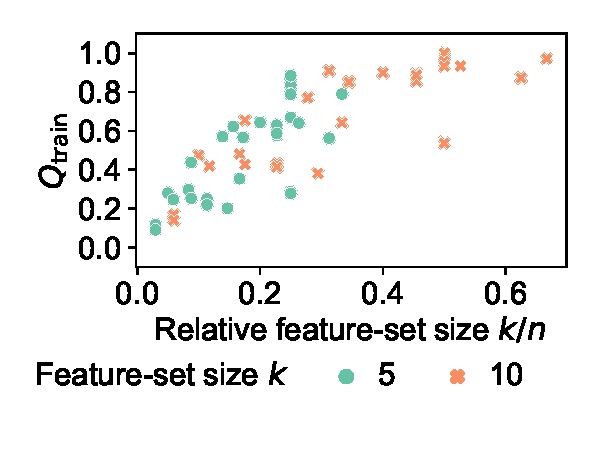
\includegraphics[width=\textwidth, trim=15 30 15 15, clip]{plots/afs-impact-dataset-k-train-objective.pdf}
		\caption{Training-set objective value.}
		\label{fig:afs:impact-dataset-k-train-objective}
	\end{subfigure}
	\hfill
	\begin{subfigure}[t]{0.48\textwidth}
		\centering
		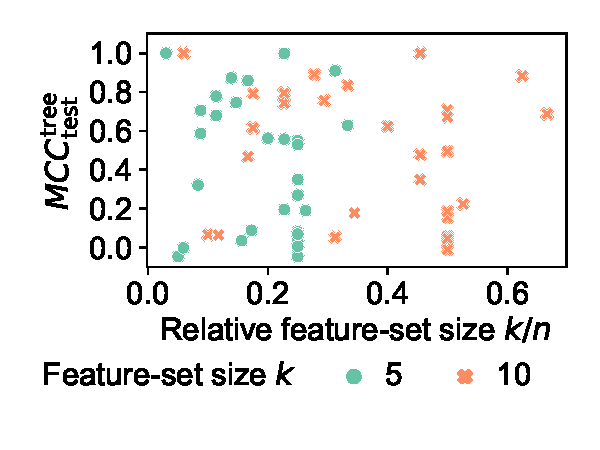
\includegraphics[width=\textwidth, trim=15 30 15 15, clip]{plots/afs-impact-dataset-k-decision-tree-test-mcc.pdf}
		\caption{Test-set prediction performance.}
		\label{fig:afs:impact-dataset-k-decision-tree-test-mcc}
	\end{subfigure}
	\caption{
		Feature-set quality over feature-set size~$k$ relative to dataset dimensionality~$n$.
		Results from the original feature sets of sequential search with \emph{MI} as feature-selection method.
	}
	\label{fig:afs:impact-dataset-k-quality}
\end{figure}

Naturally, feature-set quality depends on the datasets used, and several effects could occur.
For example, the distribution of feature-set quality in the datasets might be relatively uniform or relatively skewed.
Datasets with more features $n$ give way to more alternative feature sets.
At the same time, the feature quality can be spread over more features than for smaller datasets, making it harder to compose a small high-quality feature set.

Indeed, our experiments show a broad variation of feature-set quality over the datasets.
Figure~\ref{fig:afs:impact-dataset-k-quality} depicts the relationship between datasets and quality of the original feature set in sequential search.
To account for the varying number of features in the dataset, we put the ratio between feature-set size~$k$ and dataset dimensionality~$n$ on the x-axis, which is a measure of relative feature-set sizes.
As Figure~\ref{fig:afs:impact-dataset-k-train-objective} displays, the objective of an univariate feature-selection method approximately increases linearly with~$k/n$.
However, there still is some variation exclusively caused by the dataset rather than its dimensionality.
Further, the quality of a prediction model, i.e., decision trees, does not exhibit any trend but varies strongly between datasets, as Figure~\ref{fig:afs:impact-dataset-k-decision-tree-test-mcc} visualizes.
Due to this variance caused by dataset choice, we additionally normalize feature-set quality in some of the following analyses.
In particular, this normalization should reduce the influence of datasets and highlight the impact of other experimental settings instead.

\subsection{Feature-Set Quality Metrics}
\label{sec:afs:evaluation:metrics}

\begin{figure}[htb]
	\centering
	\begin{subfigure}[t]{0.48\textwidth}
		\centering
		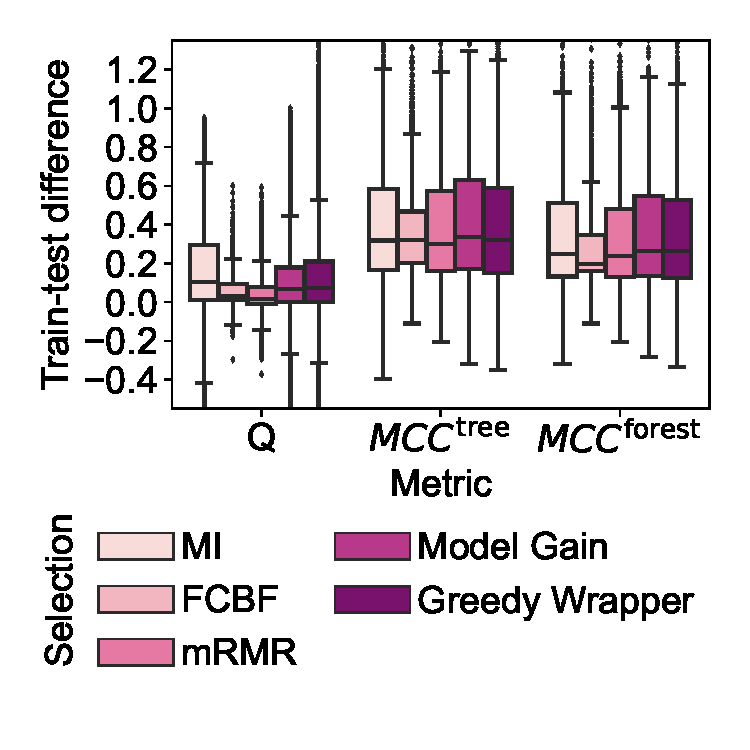
\includegraphics[width=\textwidth, trim=15 15 15 15, clip]{plots/afs-evaluation-metrics-overfitting.pdf}
		\caption{
			Training-test difference in feature-set quality by feature-selection method.
			Y-axis truncated to improve readability.
		}
		\label{fig:afs:evaluation-metrics-overfitting}
	\end{subfigure}
	\hfill
	\begin{subfigure}[t]{0.48\textwidth}
		\centering
		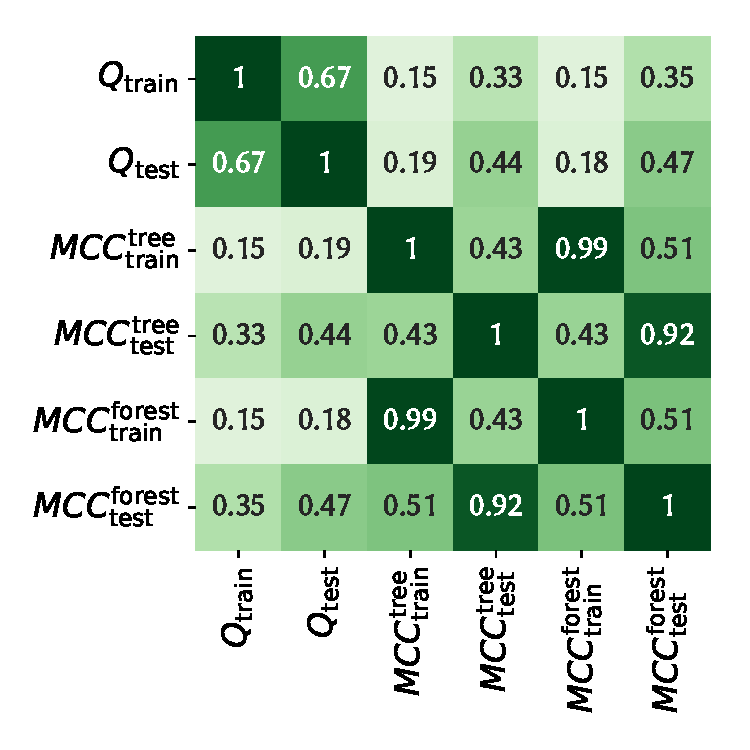
\includegraphics[width=\textwidth, trim=15 15 15 15, clip]{plots/afs-evaluation-metrics-correlation.pdf}
		\caption{Correlation between evaluation metrics, averaged over datasets, cross-valida\-tion folds, and feature-selection methods.}
		\label{fig:afs:evaluation-metrics-correlation}
	\end{subfigure}
	\caption{
		Feature-set quality by evaluation metric.
		Results from all search runs.
	}
	\label{fig:afs:evaluation-metrics}
\end{figure}

\paragraph{Prediction models and overfitting}

As one can expect, the average prediction performance of random forests is higher than that of decision trees.
Also, overfitting occurs for both model types, i.e., there is a gap between training-set and test-set prediction performance.
In particular, over all experimental settings, decision trees and random forests both have a mean training-set MCC of 0.85 (median: 1.0).
In contrast, on the test set, decision trees have a mean MCC of 0.48 (median: 0.54), while random forests have a slightly higher mean MCC of 0.52 (median: 0.63).
Thus, average prediction performance is significantly worse on the test set than on the training set.
When analyzing prediction performance in the following, we only report test-set performance.

For a more detailed comparison, Figure~\ref{fig:afs:evaluation-metrics-overfitting} shows the distribution of the difference between training and test feature-set quality, again over all experimental settings.
Once more, we observe that training feature-set quality is usually higher, i.e., the difference displayed in the figure is greater than zero.
Nevertheless, there are a few cases where the difference becomes negative, i.e., test feature-set quality is higher.
The existence of overfitting makes sense as we do not regularize, i.e., limit the growth of, the trees or prune them after training.
However, this does not invalidate our analysis of how prediction performance develops over alternatives.
The optimization objective~$Q$, which Figure~\ref{fig:afs:evaluation-metrics-overfitting} also depicts, shows overfitting for all feature-selection methods as well, though to a lesser extent than for prediction performance, so we consider training set and test set for this evaluation metric in the following.

\paragraph{Correlation between evaluation metrics}

Figure~\ref{fig:afs:evaluation-metrics-correlation} shows the Spearman correlation between different evaluation metrics over all experimental settings:
First, we compute the correlation for each combination of dataset, cross-validation fold, and feature-selection method.
Second, we average the correlation values over these experimental dimensions.
This two step procedure accounts for the different objectives of feature-selection methods, and the normalization of quality per dataset and cross-validation fold for some quality functions (cf.~Section~\ref{sec:afs:experimental-design:approaches:feature-selection}).
The plot shows that the performance of decision trees and random forests is highly correlated on the training set as well as the test set.
Thus, we only report prediction performance of one model in the following:
We choose decision trees, as they always consider all features during training, while random forests involve random sampling of features.

Figure~\ref{fig:afs:evaluation-metrics-correlation} also shows that the correlation between training and test feature-set quality is only moderate for the optimization objective~$Q$ and weak for prediction performance in terms of MCC.
This might be caused by different degrees of overfitting, depending on the experimental settings.
Further, the correlation between optimization objective~$Q$ and prediction MCC is only weak to moderate as well.
I.e., the objective of feature selection is only partially indicative of prediction performance since the former might use a simplified quality criterion.
Among the five feature-selection methods, \emph{Greedy Wrapper} has the highest correlation between training-set objective value and test-set prediction performance, with a value of 0.43.
Since this feature-selection method uses prediction performance as the objective value, a comparatively high correlation is expected.
On the other end of the spectrum, \emph{mRMR} exhibits a correlation of -0.05 between training-set objective value and test-set prediction performance.
This filter method penalizes correlation between features in its objective.
However, with decision trees as prediction models, redundant features may not hurt prediction performance, even if they do not improve it.

\subsection{Feature-Selection Methods}
\label{sec:afs:evaluation:feature-selection}

\begin{figure}[htb]
	\centering
	\begin{subfigure}[t]{0.48\textwidth}
		\centering
		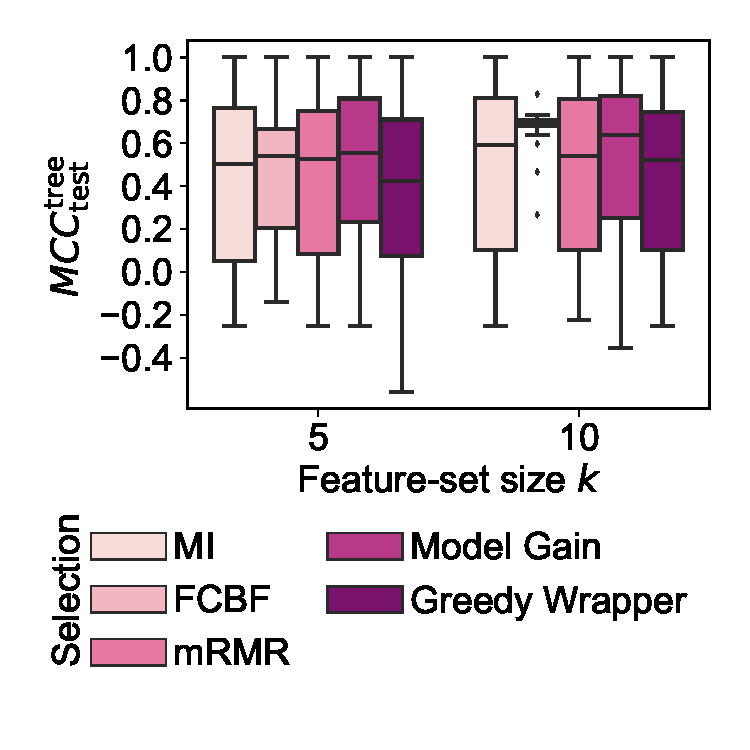
\includegraphics[width=\textwidth, trim=15 40 15 15, clip]{plots/afs-impact-fs-method-k-decision-tree-test-mcc.pdf}
		\caption{Test-set prediction performance.}
		\label{fig:afs:impact-fs-method-k-decision-tree-test-mcc}
	\end{subfigure}
	\hfill
	\begin{subfigure}[t]{0.48\textwidth}
		\centering
		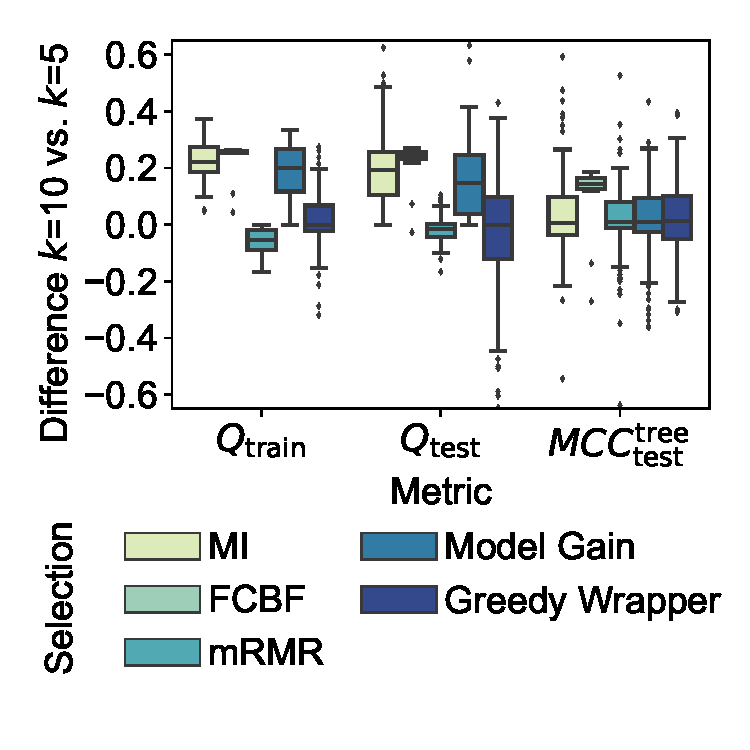
\includegraphics[width=\textwidth, trim=15 40 15 15, clip]{plots/afs-impact-fs-method-k-metric-diff.pdf}
		\caption{
			Difference in feature-set quality between $k=10$ and $k=5$ by evaluation metric.
			Y-axis truncated to improve readability.
		}
		\label{fig:afs:impact-fs-method-k-metric-diff}
	\end{subfigure}
	\caption{
		Feature-set quality by feature-selection method and feature-set size~$k$.
		Results from the original feature sets of sequential search.
	}
	\label{fig:afs:impact-fs-method-k-quality}
\end{figure}

\paragraph{Prediction performance}

As the different feature-selection methods employ different objective functions~$Q$, it does not make sense to compare absolute objective values between feature-selection methods to judge which method is best.
However, we can compare how useful the obtained feature sets are for predictions.
Figure~\ref{fig:afs:impact-fs-method-k-decision-tree-test-mcc} compares a decision tree's test-set prediction performance on the original feature sets of sequential search for different feature-selection methods.
On average, \emph{Model Gain} is the best feature-selection method, though not clearly better than the other feature-selection methods.
In particular, the median test-set MCC of decision trees is 0.59 for \emph{Model Gain}, 0.57 for \emph{FCBF}, and 0.54 for \emph{MI}, 0.53 for \emph{mRMR}, and 0.46 for \emph{Greedy Wrapper}.
In particular, the univariate, model-free feature scoring with \emph{MI} keeps up surprisingly well with the more sophisticated methods.
Thus, we focus on \emph{MI} for subsequent analyses of alternative feature sets, while still discussing the remaining feature-selection methods.
The overall best feature-selection method, \emph{Model Gain}, uses the same objective function as \emph{MI} but obtains its feature qualities from a prediction model rather than a bivariate dependency measure, which might be the crucial factor for its out-performance. 

The relatively bad performance of \emph{Greedy Wrapper} might result from its heuristic nature:
The wrapper search can only evaluate a fraction of all feasible feature sets and might get stuck in local optima, while the remaining feature-selection methods optimize globally.
In particular, \emph{Greedy Wrapper} only performed 71 iterations on average (median: 50) to determine the original feature sets of sequential search.
The figures concerning all experimental settings are similar, with a mean of 65 and a median of 45.
Thus, \emph{Greedy Wrapper} usually stayed significantly below the 1000~iterations we granted it.

Further, the results for \emph{FCBF} have to be taken with a grain of salt:
Over all experimental settings, 89\% of feature sets for \emph{FCBF} were infeasible, i.e., no feature set could satisfy the constraints.
In contrast, this figure only is 18\% for \emph{MI}.
Even the original feature set in sequential search is infeasible in 76\% of the cases for \emph{FCBF} but never for the other feature-selection methods.
In particular, the combination of feature-correlation constraints in our formulation of \emph{FCBF} (c.f.~Equation~\ref{eq:afs:fcbf}) with a feature-set-cardinality constraint, i.e., enforcing a certain feature-set size~$k$, seemingly made it hard to find valid feature sets.
This phenomenon becomes even more relevant the higher~$k$ is.

\paragraph{Influence of feature-set size~$k$}

As one can expect, larger feature sets, i.e., with~$k=10$, usually exhibit higher feature-set quality than smaller feature sets, i.e., with $k=5$.
However, the increase in feature-set quality with $k$ is not proportional, and there might even be a decrease.
As Figure~\ref{fig:afs:impact-fs-method-k-metric-diff} shows for the original feature sets of sequential search, \emph{MI}, \emph{FBCF}, and \emph{Model Gain} exhibit a slight increase of the training-set objective value~$Q_\text{train}$ from~$k=5$ to~$k=10$, i.e., the difference depicted in Figure~\ref{fig:afs:impact-fs-method-k-metric-diff} is positive.
As these objectives are monotonic in the set of selected features, a decrease in training-set quality is not possible.
In contrast, the heuristic \emph{Greedy Wrapper} does not necessarily benefit from selecting more features.
The latter insight applies to the white-box method \emph{mRMR} as well since it normalizes its objective with the number of selected features and penalizes feature redundancy.
As Figure~\ref{fig:afs:impact-fs-method-k-metric-diff} also displays, the benefit of larger feature sets is even less clear for prediction performance.
In particular, all feature-selection methods except \emph{FCBF} show a median difference in test-set MCC close to zero when comparing $k=5$ to $k=10$.
Thus, we focus on smaller feature sets, i.e., $k=5$, in the following.

\subsection{Searching Alternatives}
\label{sec:afs:evaluation:search}

In this section, we evaluate the different choices for searching alternatives: the search method (cf.~Section~\ref{sec:afs:evaluation:search:method}), number of alternatives~$a$ (cf.~Section~\ref{sec:afs:evaluation:search:num-alternatives}), and dissimilarity threshold~$\tau$ (cf.~Section~\ref{sec:afs:evaluation:search:tau}).

\subsubsection{Search Methods for Alternatives}
\label{sec:afs:evaluation:search:method}

\begin{figure}[p]
	\centering
	\begin{subfigure}[t]{0.48\textwidth}
		\centering
		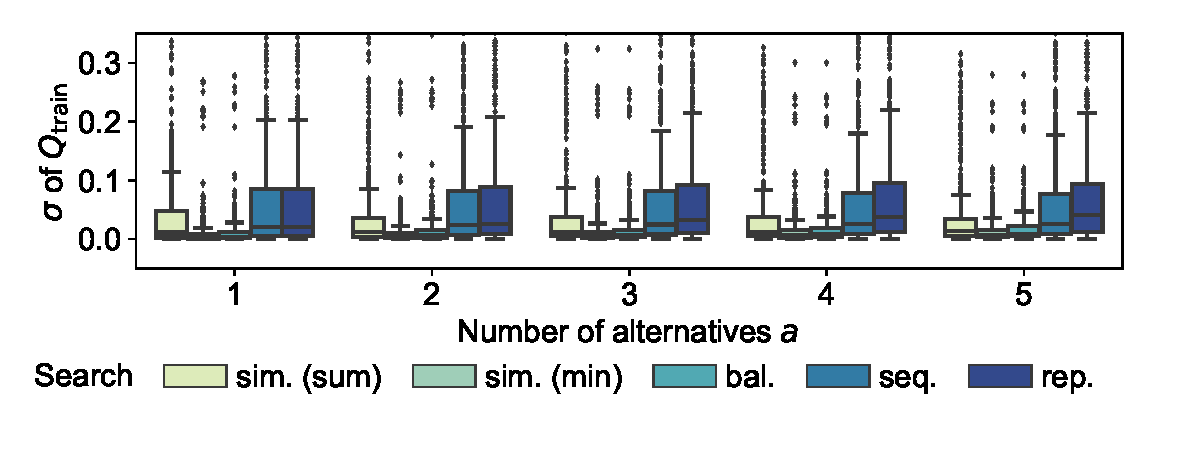
\includegraphics[width=\textwidth, trim=15 25 15 10, clip]{plots/afs-impact-search-stddev-train-objective.pdf}
		\caption{Standard deviation of training-set objective value within search runs.}
		\label{fig:afs:impact-search-stddev-train-objective}
	\end{subfigure}
	\hfill
	\begin{subfigure}[t]{0.48\textwidth}
		\centering
		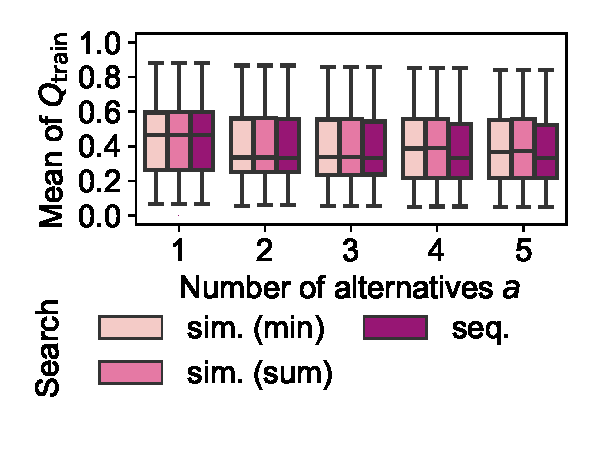
\includegraphics[width=\textwidth, trim=15 25 15 10, clip]{plots/afs-impact-search-mean-train-objective.pdf}
		\caption{Mean of training-set objective value within search runs.}
		\label{fig:afs:impact-search-mean-train-objective}
	\end{subfigure}
	\\ \vspace{\baselineskip}
	\begin{subfigure}[t]{0.48\textwidth}
		\centering
		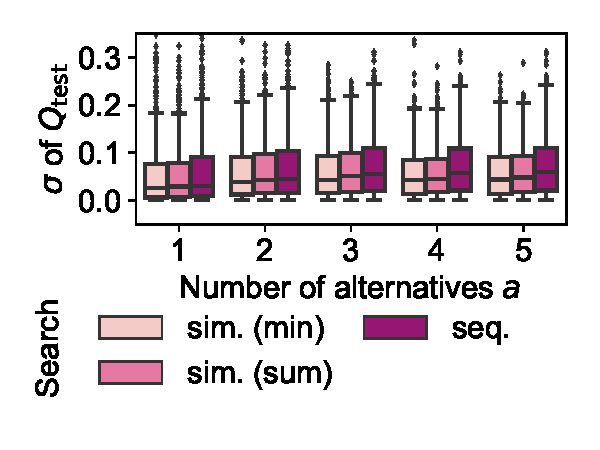
\includegraphics[width=\textwidth, trim=15 25 15 15, clip]{plots/afs-impact-search-stddev-test-objective.pdf}
		\caption{Standard deviation of test-set objective value within search runs.}
		\label{fig:afs:impact-search-stddev-test-objective}
	\end{subfigure}
	\hfill
	\begin{subfigure}[t]{0.48\textwidth}
		\centering
		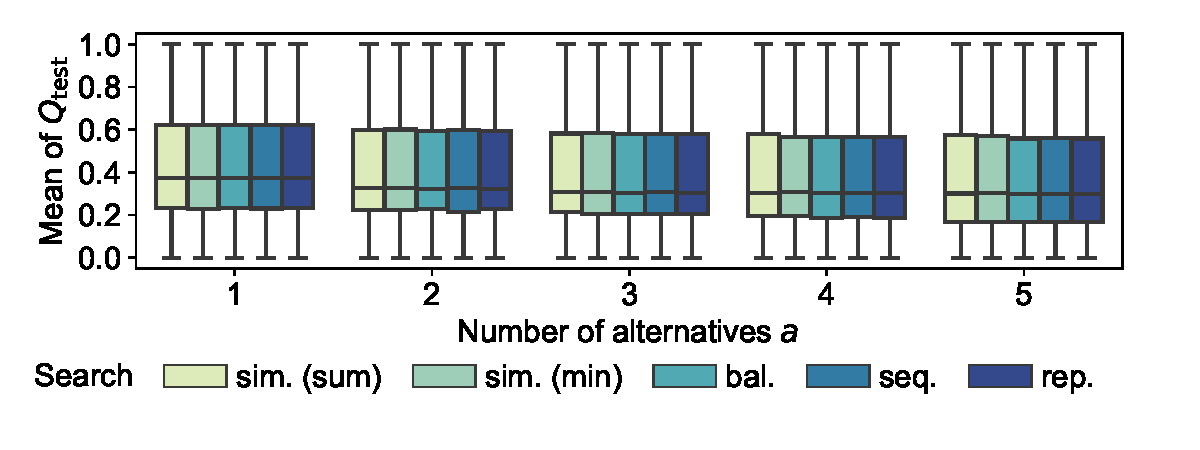
\includegraphics[width=\textwidth, trim=15 25 15 15, clip]{plots/afs-impact-search-mean-test-objective.pdf}
		\caption{Mean of test-set objective value with\-in search runs.}
		\label{fig:afs:impact-search-mean-test-objective}
	\end{subfigure}
	\\ \vspace{\baselineskip}
	\begin{subfigure}[t]{0.48\textwidth}
		\centering
		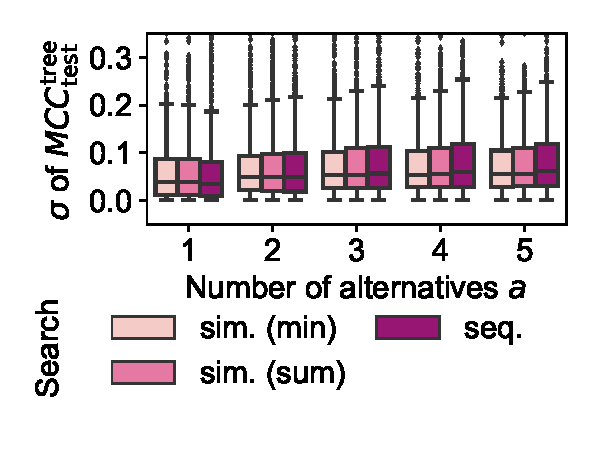
\includegraphics[width=\textwidth, trim=15 25 15 5, clip]{plots/afs-impact-search-stddev-decision-tree-test-mcc.pdf}
		\caption{Standard deviation of test-set prediction performance within search runs.}
		\label{fig:afs:impact-search-stddev-decision-tree-test-mcc}
	\end{subfigure}
	\hfill
	\begin{subfigure}[t]{0.48\textwidth}
		\centering
		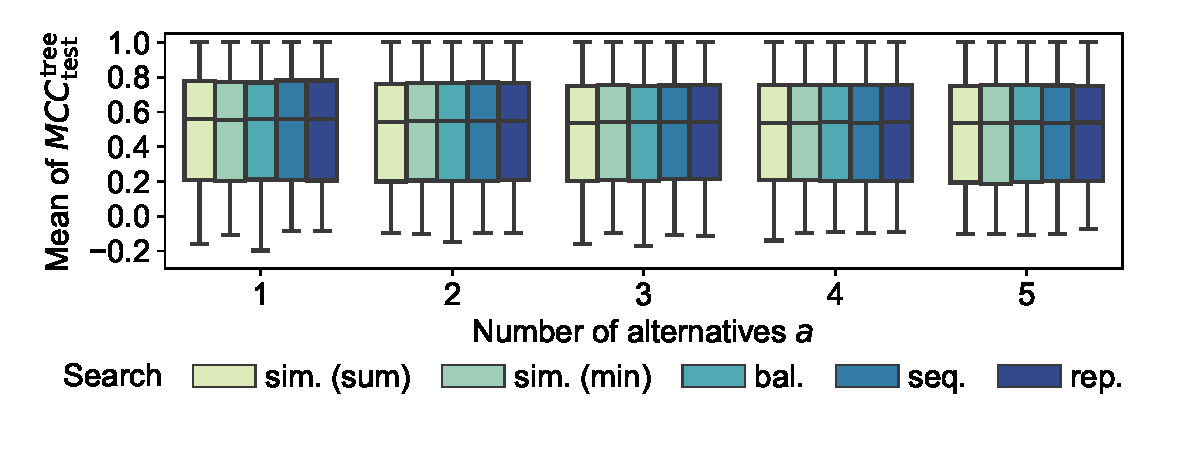
\includegraphics[width=\textwidth, trim=15 25 15 5, clip]{plots/afs-impact-search-mean-decision-tree-test-mcc.pdf}
		\caption{Mean of test-set prediction performance within search runs.}
		\label{fig:afs:impact-search-mean-decision-tree-test-mcc}
	\end{subfigure}
	\caption{
		Feature-set quality over the number of alternatives, by evaluation metric and search method for alternatives.
		Results with \emph{MI} as feature-selection method and $k=5$.
		Y-axes truncated to improve readability.
	}
	\label{fig:afs:impact-search-quality}
\end{figure}

\begin{figure}[htb]
	\centering
	\begin{subfigure}[t]{0.48\textwidth}
		\centering
		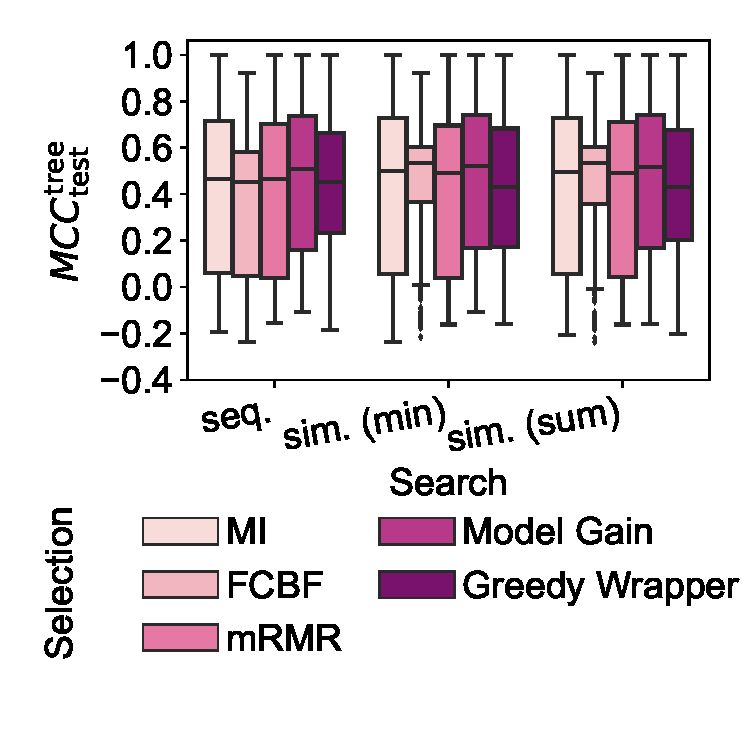
\includegraphics[width=\textwidth, trim=15 40 15 10, clip]{plots/afs-impact-search-fs-method-decision-tree-test-mcc.pdf}
		\caption{Test-set prediction performance.}
		\label{fig:afs:impact-search-fs-method-decision-tree-test-mcc}
	\end{subfigure}
	\hfill
	\begin{subfigure}[t]{0.48\textwidth}
		\centering
		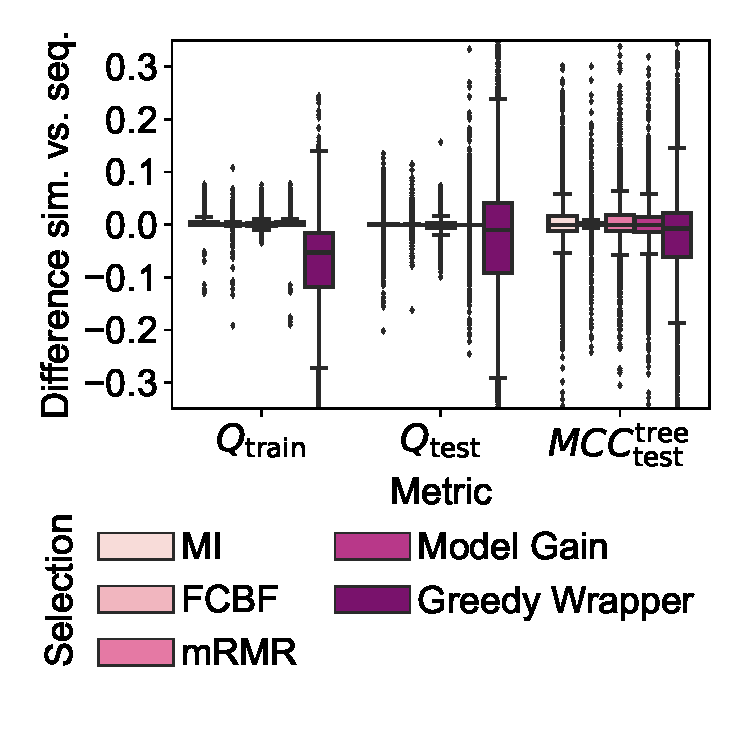
\includegraphics[width=\textwidth, trim=15 40 15 10, clip]{plots/afs-impact-search-fs-method-metric-diff.pdf}
		\caption{
			Difference in feature-set quality between simultaneous (sum-aggregation) and sequential search by evaluation metric.
			Y-axis truncated to improve readability.
		}
		\label{fig:afs:impact-search-fs-method-metric-diff}
	\end{subfigure}
	\caption{
		Feature-set quality by feature-selection method and search method for alternatives.
		Results with $k=5$ and $a \in \{1,2,3,4,5\}$.
	}
	\label{fig:afs:impact-search-fs-method-quality}
\end{figure}

\paragraph{Variance in feature-set quality}

As expected, the choice of the search method influences how much the training-set objective value~$Q$ varies between alternatives found within each search run.
Figure~\ref{fig:afs:impact-search-stddev-train-objective} visualizes this observation for \emph{MI} as feature-selection method and $k=5$.
In particular, multiple alternative feature sets found by sequential search usually vary more in their quality than for simultaneous search.
When using simultaneous search, min-aggregation yields significantly more homogeneous feature-set quality than sum-aggregation.
These findings apply to all white-box feature-selection methods but not the heuristic \emph{Greedy Wrapper}.

As Figures~\ref{fig:afs:impact-search-stddev-test-objective} and~\ref{fig:afs:impact-search-stddev-decision-tree-test-mcc} show, the difference between the search methods is clearly less prominent when observing the variance of feature-set quality on the test set.
This observation applies to quality in terms of objective value as well as prediction performance.
In particular, alternatives found by simultaneous search do not have considerably more homogeneous test feature-set quality than for sequential search.
This effect might be a result of overfitting:
Even if training feature-set quality is similar, some alternatives might generalize better, i.e., maintain their quality on the test set, while other alternatives might loose quality to a larger extent.
Thus, the variance in test feature-set quality caused by overfitting could alleviate the effect on variance caused by the search method.

\paragraph{Average value of feature-set quality}

While obtaining alternatives of more homogeneous quality can be one goal of simultaneous search, the main selling point would be obtaining alternatives of higher average quality.
However, we found that simultaneous search is not clearly better than sequential search in that regard.
In particular, Figure~\ref{fig:afs:impact-search-mean-train-objective} compares the distribution of the mean training-set objective in search runs for \emph{MI} as feature-selection method and $k=5$.
We observe that all search methods yield very similar distribution of training-set objective values.
This observation holds for all four white-box feature selection methods, while the heuristic \emph{Greedy Wrapper} even favors sequential search over simultaneous search.
In contrast, for \emph{MI}, as visible in Figure~\ref{fig:afs:impact-search-mean-train-objective}, and \emph{Model Gain}, simultaneous search tends to develop a slight advantage over sequential search at least with a growing number of alternatives.

The negligible quality difference between the search methods is also visible for the test-set objective value in Figure~\ref{fig:afs:impact-search-mean-test-objective} and the test-set prediction performance in Figure~\ref{fig:afs:impact-search-mean-decision-tree-test-mcc}.
In particular, as Figure~\ref{fig:afs:impact-search-fs-method-decision-tree-test-mcc} displays, other aspects of the experimental design, e.g., dataset, dissimilarity threshold~$\tau$, etc. cause a variation in prediction performance that exceeds the variation between the search methods.

As a final quality comparison, Figure~\ref{fig:afs:impact-search-fs-method-metric-diff} displays the difference in feature-set quality between sequential and simultaneous search if it is compared on each search setting separately, i.e., each combination of dataset, fold, dissimilarity threshold~$\tau$, etc.
The figure again shows that all feature-selection methods except \emph{Greedy Wrapper} exhibit little variation in quality between these two search approaches, apart from some outlying experimental settings, i.e., the difference in feature-set quality is usually close to zero.
Additionally, the figure highlights that outliers can occur in both directions:
While simultaneous search can yield better-performing feature sets in some situations, sequential search can be significantly better in other scenarios.

\begin{table}[htb]
	\centering
	\begin{tabular}{llrrrr}
		\toprule
		Selection & Search & \multicolumn{4}{c}{Optimization status} \\
		\cmidrule(r){3-6}
		& & Infeasible & Not solved & Feasible & Optimal \\
		\midrule
		FCBF & seq. & 70.25\% & 0.00\% & 0.00\% & 29.75\% \\
		FCBF & sim. (min) & 74.13\% & 0.08\% & 1.45\% & 24.33\% \\
		FCBF & sim. (sum) & 74.12\% & 0.09\% & 2.01\% & 23.77\% \\
		MI & seq. & 1.97\% & 0.00\% & 0.00\% & 98.03\% \\
		MI & sim. (min) & 4.67\% & 0.00\% & 8.80\% & 86.53\% \\
		MI & sim. (sum) & 4.67\% & 0.00\% & 2.44\% & 92.89\% \\
		Model Gain & seq. & 1.97\% & 0.00\% & 0.00\% & 98.03\% \\
		Model Gain & sim. (min) & 4.67\% & 0.00\% & 5.25\% & 90.08\% \\
		Model Gain & sim. (sum) & 4.67\% & 0.00\% & 1.75\% & 93.59\% \\
		mRMR & seq. & 1.96\% & 0.00\% & 9.90\% & 88.14\% \\
		mRMR & sim. (min) & 4.67\% & 0.00\% & 48.72\% & 46.61\% \\
		mRMR & sim. (sum) & 4.67\% & 0.00\% & 66.99\% & 28.35\% \\
		\bottomrule
	\end{tabular}
	\caption{
		Frequency of optimization statuses (cf.~Section~\ref{sec:afs:experimental-design:evaluation}) by feature-selection method and search method for alternatives.
		Results with $k=5$ and $a \in \{1,2,3,4,5\}$.
		Excluding \emph{Greedy Wrapper}, which calls the solver multiple times, and checks satisfiability rather than optimizing.
		Each row sums to 100\%.
	}
	\label{tab:afs:impact-search-fs-method-optimization-status}
\end{table}
%
\begin{table}[htb]
	\centering
	\begin{tabular}{rrrrr}
		\toprule
		$a$ & \multicolumn{4}{c}{Optimization status} \\
		\cmidrule(r){2-5}
		& Infeasible & Not solved & Feasible & Optimal \\
		\midrule
		1 & 16.88\% & 0.00\% & 7.45\% & 75.67\% \\
		2 & 17.97\% & 0.00\% & 13.63\% & 68.40\% \\
		3 & 20.20\% & 0.00\% & 20.03\% & 59.77\% \\
		4 & 26.90\% & 0.02\% & 21.42\% & 51.67\% \\
		5 & 28.20\% & 0.10\% & 28.95\% & 42.75\% \\
		\bottomrule
	\end{tabular}
	\caption{
		Frequency of optimization statuses (cf.~Section~\ref{sec:afs:experimental-design:evaluation}) by number of alternatives~$a$.
		Results from simultaneous search with sum-aggregation and $k=5$, excluding \emph{Greedy Wrapper} as feature-selection method.
		Each row sums to 100\%.
	}
	\label{tab:afs:impact-num-alternatives-optimization-status}
\end{table}

\paragraph{Optimization status}

A major reason for simultaneous search failing to consistently beat sequential search quality-wise is that search results can be sub-optimal.
For \emph{Greedy Wrapper}, the search is heuristic per se, and only a tiny fraction of the search space is covered.
For all feature-selection methods, the solver can time out.
As the optimization problem of simultaneous search is harder than for sequential search (cf.~Table~\ref{tab:afs:seq-sim-comparison}), it has a higher likelihood to run into timeouts.
Table~\ref{tab:afs:impact-search-fs-method-optimization-status} visualizes this phenomenon.
In particular, for up to five alternatives and $k=5$, all sequential searches for \emph{FCBF}, \emph{MI}, and \emph{Model Gain} finished within the timeout, i.e., yielded the optimal feature set or ascertained infeasibility.
For \emph{mRMR}, there are about 10\% potentially suboptimal feature sets under the same settings.
In contrast, for simultaneous search with sum-aggregation, all feature-selection methods experience timeouts in searches:
Roughly 2\% of the searches for \emph{FCBF}, \emph{MI}, and \emph{Model Gain}, and 67\% of the searches for \emph{mRMR} found a feasible solution till the timeout but could not guarantee optimality.
Such timeout-affected solutions of simultaneous search can be worse than an optimal sequential solution.
With min-aggregation instead of sum-aggregation in simultaneous search, the number of timeouts increases for \emph{MI} and \emph{Model Gain} but decreases for \emph{FCBF} and \emph{mRMR}.
Still, sequential search runs into less timeouts for all four white-box feature-selection methods.

Besides finding suboptimal feature sets, the solver might also fail to find a feasible solution without being able to guarantee infeasibility.
However, this optimization status, called \emph{not solved}, occurred rarely in our experiments, and only for \emph{FCBF} in simultaneous search.
Further, note that the fraction of timeouts strongly depends on the number of alternatives~$a$, as Table~\ref{tab:afs:impact-num-alternatives-optimization-status} displays:
For simultaneous search with $k=5$ and sum-aggregation, roughly 7\% of the white-box searches timed out for one alternative but 20\% for three alternatives and 29\% for five alternatives.
Remember that we grant simultaneous searches proportionally more time to obtain more feature sets.
The nevertheless observed increase in timeouts suggests that runtime increases super-proportionally, as we analyze next.

\begin{table}[htb]
	\centering
	\begin{tabular}{lrrr}
		\toprule
		Selection & \multicolumn{3}{c}{Optimization time} \\
		\cmidrule(r){2-4}
		& seq. & sim. (min) & sim. (sum) \\
		\midrule
		FCBF & 0.18~s & 11.55~s & 13.40~s \\
		Greedy Wrapper & 6.96~s & 10.67~s & 11.48~s \\
		MI & 0.02~s & 44.21~s & 22.46~s \\
		Model Gain & 0.02~s & 30.26~s & 19.52~s \\
		mRMR & 35.78~s & 155.62~s & 189.29~s \\
		\bottomrule
	\end{tabular}
	\caption{
		Mean optimization time by feature-selection method and search method for alternatives.
		Results with $k=5$ and $a \in \{1,2,3,4,5\}$.
	}
	\label{tab:afs:impact-search-fs-method-optimization-time}
\end{table}
%
\begin{table}[htb]
	\centering
	\begin{tabular}{lrrrrr}
		\toprule
		$a$ & \multicolumn{5}{c}{Optimization time} \\
		\cmidrule(r){2-6}
		& FCBF & Wrapper & MI & Model Gain & mRMR \\
		\midrule
		1 & 0.42~s & 3.20~s & 0.02~s & 0.02~s & 44.96~s \\
		2 & 0.91~s & 5.07~s & 0.07~s & 0.06~s & 119.42~s \\
		3 & 3.11~s & 7.56~s & 0.25~s & 0.23~s & 206.00~s \\
		4 & 14.98~s & 18.69~s & 3.73~s & 3.43~s & 258.60~s \\
		5 & 47.57~s & 22.87~s & 108.22~s & 93.89~s & 317.44~s \\
		\bottomrule
	\end{tabular}
	\caption{
		Mean optimization time by feature-selection method and number of alternatives~$a$.
		Results from simultaneous search with sum-aggregation and $k=5$.
	}
	\label{tab:afs:impact-num-alternatives-fs-method-optimization-time}
\end{table}

\paragraph{Optimization time}

Analyzing the actual optimization time instead of the optimization status also speaks in favor of sequential search.
As Table~\ref{tab:afs:impact-search-fs-method-optimization-time} shows, the mean optimization time of sequential search is lower for all five feature-selection methods.
In particular, the difference in mean optimization time between sequential and simultaneous search is up to three orders of magnitude for the four white-box feature-selection methods.
Further, \emph{MI}, and \emph{Model Gain} experiences a dramatic, clearly super-linear increase in mean optimization time with the number of alternatives~$a$ in simultaneous search, as Table~\ref{tab:afs:impact-num-alternatives-fs-method-optimization-time} displays.
In contrast, the runtime increase is considerably less for sequential search since it shows an approximately linear trend with the number of alternatives there.

Based on all results described in this section, we focus on the sequential search in the following.
In particular, it appeared to be significantly faster than simultaneous search while yielding similar feature-set quality.

Another interesting question for practitioners is how the runtime relates to~$n$, the total number of features in the dataset.
One would expect a positive correlation, since the optimization problem's instance size increases with~$n$.
Roughly speaking, this trend also appears in our experimental data.
However, the observed trend does not match a simple functional relationship, and some higher-dimensional datasets even show lower average runtimes than lower-dimensional datasets.
This indicates that several other factors apart from~$n$ influence solver runtime.
Besides factors related to our experimental design and the datasets, the heuristics employed by the solver might also play a role, e.g., work better for some problem instances than for others.

\subsubsection{Number of Alternatives \texorpdfstring{$a$}{}}
\label{sec:afs:evaluation:search:num-alternatives}

\begin{figure}[p]
	\centering
	\begin{subfigure}[t]{\textwidth}
		\centering
		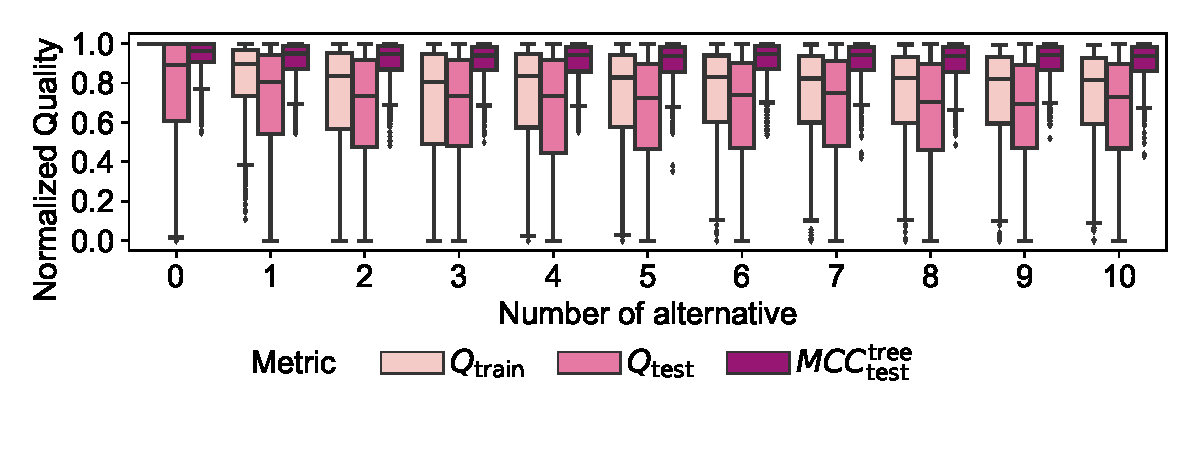
\includegraphics[width=\textwidth, trim=15 30 15 15, clip]{plots/afs-impact-num-alternatives-quality-max.pdf}
		\caption{Max-normalized, infeasible feature sets excluded.}
		\label{fig:afs:impact-num-alternatives-quality-max}
	\end{subfigure}
	\begin{subfigure}[t]{\textwidth}
		\centering
		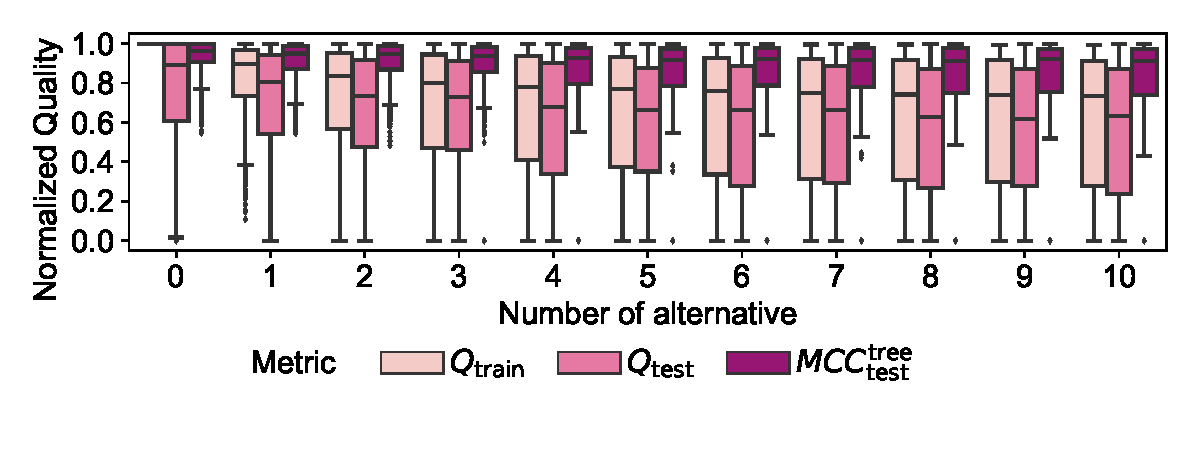
\includegraphics[width=\textwidth, trim=15 30 15 15, clip]{plots/afs-impact-num-alternatives-quality-max-fillna.pdf}
		\caption{Max-normalized, infeasible feature sets assigned a quality of~0.}
		\label{fig:afs:impact-num-alternatives-quality-max-fillna}
	\end{subfigure}
	\begin{subfigure}[t]{\textwidth}
		\centering
		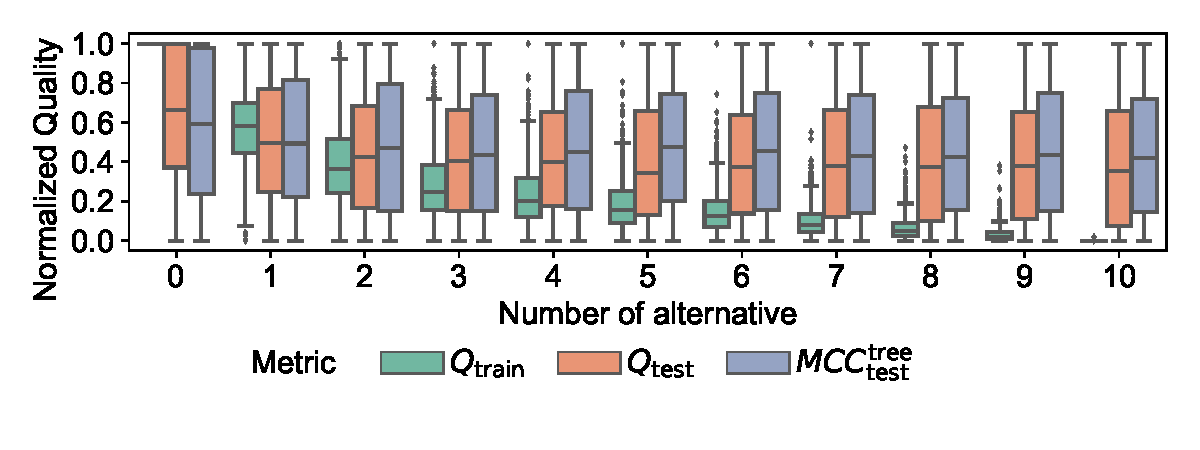
\includegraphics[width=\textwidth, trim=15 30 15 15, clip]{plots/afs-impact-num-alternatives-quality-min-max.pdf}
		\caption{Min-max-normalized, infeasible feature sets excluded.}
		\label{fig:afs:impact-num-alternatives-quality-min-max}
	\end{subfigure}
	\begin{subfigure}[t]{\textwidth}
		\centering
		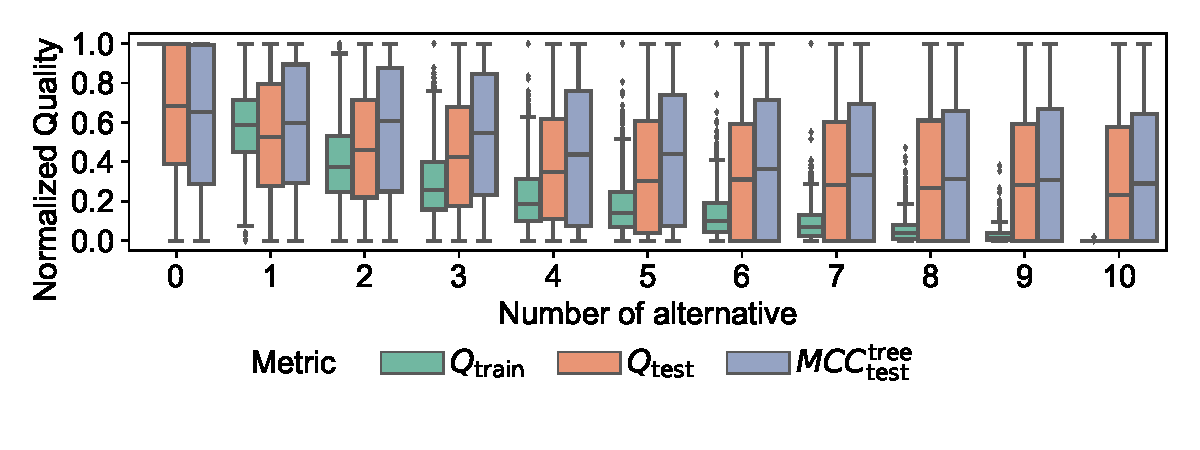
\includegraphics[width=\textwidth, trim=15 30 15 15, clip]{plots/afs-impact-num-alternatives-quality-min-max-fillna.pdf}
		\caption{Min-max-normalized, infeasible feature sets assigned a quality of~0.}
		\label{fig:afs:impact-num-alternatives-quality-min-max-fillna}
	\end{subfigure}
	\caption{
		Feature-set quality, normalized per experimental setting, over the number of alternatives, by evaluation metric.
		Results from sequential search with \emph{MI} as feature-selection method and $k=5$.
	}
	\label{fig:afs:impact-num-alternatives-quality}
\end{figure}

\paragraph{Feature-set quality}

For sequential search, the training-set objective value naturally decreases with the number of alternatives, at least for the feature-selection criteria optimized exactly.
In particular, each found feature set adds another constraint to the optimization problem.
Figures~\ref{fig:afs:impact-num-alternatives-quality-max} and~\ref{fig:afs:impact-num-alternatives-quality-min-max} illustrate this trend for \emph{MI}-based feature selection.
Since feature-set quality varies between datasets and cross-validation folds, as discussed in Section~\ref{sec:afs:evaluation:datasets}, we additionally normalize feature-set quality here.
In particular, we analyze the relative development of feature-set quality within individual search runs for alternatives.
First, we shift the range of all evaluation metrics to~$[0,1]$.
In particular, MCC to measure prediction performance as well as the objective value of \emph{Greedy Wrapper} and \emph{mRMR} would have the range~$[-1,1]$ without this shift.
Second, in Figure~\ref{fig:afs:impact-num-alternatives-quality-max}, we have max-normalized the feature-set quality for each search of alternatives, i.e., the highest feature-set quality in the search run is scaled to~1 and the other feature-set qualities are scaled accordingly.
This figure shows that there might be multiple alternatives of similar quality, as the median training-set objective value remains relatively stable over the number of alternatives.
In particular, the median training-set objective value remains relative close to the maximum of~1 and is above 0.8 even for the tenth alternative.
For comparison, Figure~\ref{fig:afs:impact-num-alternatives-quality-min-max} uses min-max normalization, i.e., the worst of the alternatives gets~0 as objective.
This figure makes the decrease in objective value over the number of alternatives more visible.
In particular, this figure highlights that the training-set objective value decreases most from the original feature set to the first alternative but less beyond.

Additionally, Figures~\ref{fig:afs:impact-num-alternatives-quality-max} and~\ref{fig:afs:impact-num-alternatives-quality-min-max} show that the test-set objective value also drops most from the original feature set to the first alternative.
However, the decrease in median test-set objective value over the alternatives only occurs for the first few alternatives.
For further alternatives, the median test-set objective value is stable.
Additionally, the initial decrease in quality is less prominent than on the training set.
In particular, alternatives can even have a higher test-set objective value than the original feature set due to overfitting.
Similar findings hold for test-set prediction performance.
Overall, these results indicate that alternative feature sets fulfill their purpose of being different solutions with similar quality as the original feature set.

\paragraph{Optimization status}

Be aware that these observations refer to the quality of the found feature sets.
However, the more alternatives are desired, the more likely an infeasible optimization problem is.
For example, the \emph{MI} feature-selection method in sequential search always finds an original feature set.
However, with $k=5$, the problem is infeasible in 2\% of the cases for the third alternative, 12\% for the fifth alternative, and 17\% for the tenth alternative.
Increasing the feature-set size $k$, e.g., to $k=10$, or decreasing the dataset dimensionality~$n$, naturally increases the number of infeasible solutions, as less features become available for alternatives.
Thus, while the quality of actually found feature sets seems to remain relatively stable with an increased number of alternatives, valid alternatives might simply not exist.
Figures~\ref{fig:afs:impact-num-alternatives-quality-max-fillna} and~\ref{fig:afs:impact-num-alternatives-quality-min-max-fillna} show the same data as Figures~\ref{fig:afs:impact-num-alternatives-quality-max} and~\ref{fig:afs:impact-num-alternatives-quality-min-max} except with the quality of infeasible feature sets set to zero, i.e., the theoretical minimum after we shifted the value ranges of all evaluation metrics.
In these figures, the downward trend of feature-set quality over the number of alternatives becomes slightly more prominent, particular for a high number of alternatives.
This downward trend also depends on the dissimilarity threshold~$\tau$, which we analyze in the next section.

\begin{figure}[htbp]
	\centering
	\begin{subfigure}[t]{0.48\textwidth}
		\centering
		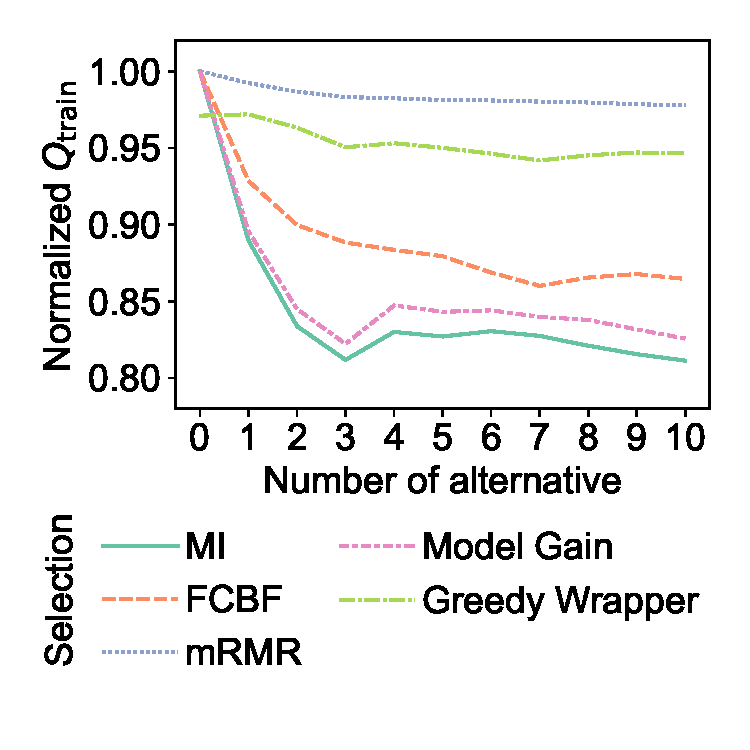
\includegraphics[width=\textwidth, trim=20 40 15 15, clip]{plots/afs-impact-num-alternatives-fs-method-train-objective-max.pdf}
		\caption{
			Training-set objective value.
			Infeasible feature sets excluded.
		}
		\label{fig:afs:impact-num-alternatives-fs-method-train-objective-max}
	\end{subfigure}
	\hfill
	\begin{subfigure}[t]{0.48\textwidth}
		\centering
		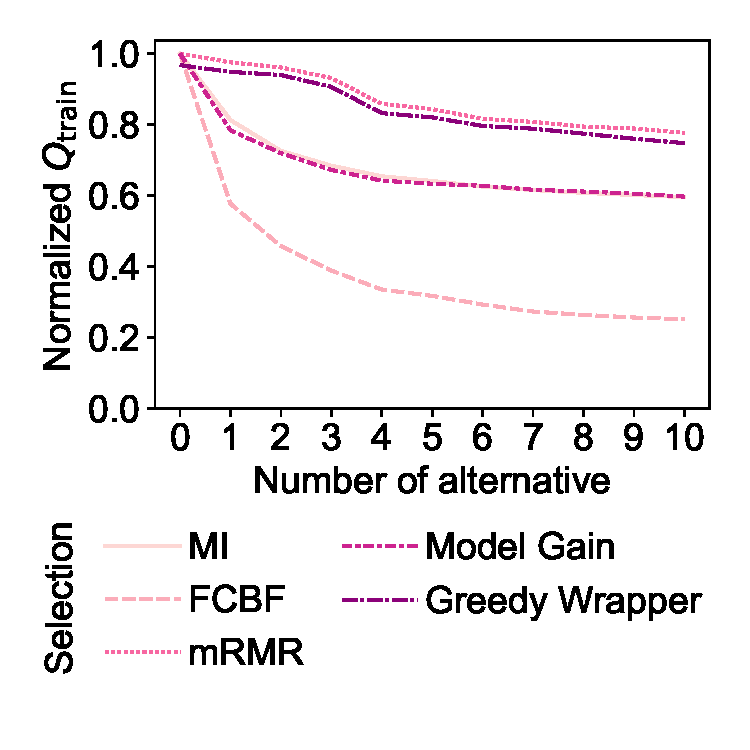
\includegraphics[width=\textwidth, trim=20 40 15 15, clip]{plots/afs-impact-num-alternatives-fs-method-train-objective-max-fillna.pdf}
		\caption{
			Training-set objective value.
			Infeasible feature sets assigned a quality of~0.
		}
		\label{fig:afs:impact-num-alternatives-fs-method-train-objective-max-fillna}
	\end{subfigure}
	\\ \vspace{\baselineskip}
	\begin{subfigure}[t]{0.48\textwidth}
		\centering
		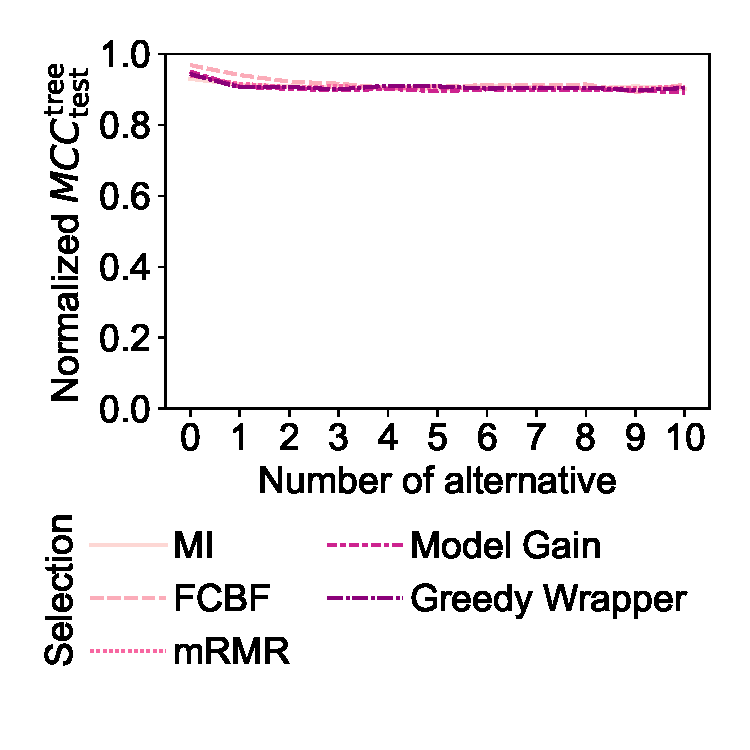
\includegraphics[width=\textwidth, trim=20 40 15 15, clip]{plots/afs-impact-num-alternatives-fs-method-decision-tree-test-mcc-max.pdf}
		\caption{
			Test-set prediction performance.
			Infeasible feature sets excluded.
		}
		\label{fig:afs:impact-num-alternatives-fs-method-decision-tree-test-mcc-max}
	\end{subfigure}
	\hfill
	\begin{subfigure}[t]{0.48\textwidth}
		\centering
		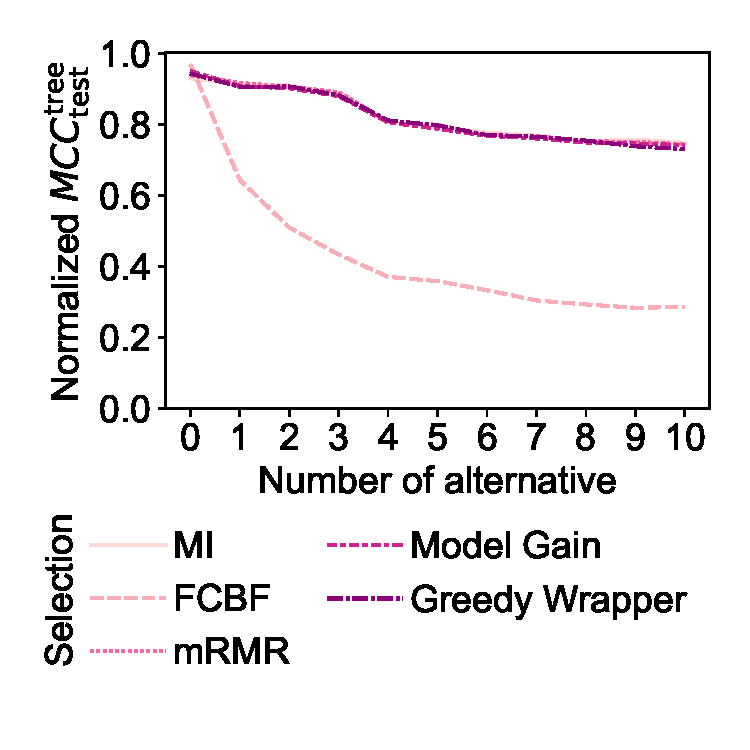
\includegraphics[width=\textwidth, trim=20 40 15 15, clip]{plots/afs-impact-num-alternatives-fs-method-decision-tree-test-mcc-max-fillna.pdf}
		\caption{
			Test-set prediction performance.
			Infeasible feature sets assigned a quality of~0.
		}
		\label{fig:afs:impact-num-alternatives-fs-method-decision-tree-test-mcc-max-fillna}
	\end{subfigure}
	\caption{
		Mean feature-set quality, max-normalized per experimental setting, over the number of alternatives, by evaluation metric and feature-selection method.
		Results from sequential search with $k=5$.
	}
	\label{fig:afs:impact-num-alternatives-fs-method-quality}
\end{figure}

\paragraph{Influence of feature-selection method}

While we discussed \emph{MI} before, the decrease of objective value over the number of alternatives occurs for all feature-selection methods in our experiments, as Figure~\ref{fig:afs:impact-num-alternatives-fs-method-train-objective-max} shows.
The strength of the decrease varies between the feature selection methods.
For example, \emph{Greedy Wrapper} and \emph{mRMR} show little effect of increasing the number alternatives, while \emph{MI} and \emph{Model Gain} exhibit the strongest effect.
As Figure~\ref{fig:afs:impact-num-alternatives-fs-method-train-objective-max-fillna} shows, the quality decrease becomes more prominent if one considers infeasible feature sets to have a quality of~0.
Further, for the test-set prediction performance, displayed in Figure~\ref{fig:afs:impact-num-alternatives-fs-method-decision-tree-test-mcc-max} none of the feature-selection methods exhibits a strong decrease over the number of alternatives, unless we account for infeasible feature sets (cf.~Figure~\ref{fig:afs:impact-num-alternatives-fs-method-decision-tree-test-mcc-max-fillna}).

\subsubsection{Dissimilarity Threshold \texorpdfstring{$\tau$}{}} % \texorpdfstring prevents warning "Token not allowed in a PDF string"
\label{sec:afs:evaluation:search:tau}

\begin{figure}[p]
	\centering
	\begin{subfigure}[t]{0.48\textwidth}
		\centering
		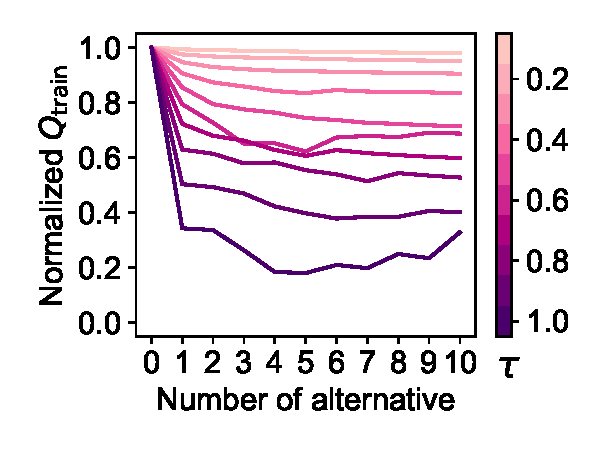
\includegraphics[width=\textwidth, trim=15 15 10 15, clip]{plots/afs-impact-num-alternatives-tau-train-objective-max.pdf}
		\caption{
			Training-set objective value, max-normalized.
			Infeasible feature sets excluded.
		}
		\label{fig:afs:impact-num-alternatives-tau-train-objective-max}
	\end{subfigure}
	\hfill
	\begin{subfigure}[t]{0.48\textwidth}
		\centering
		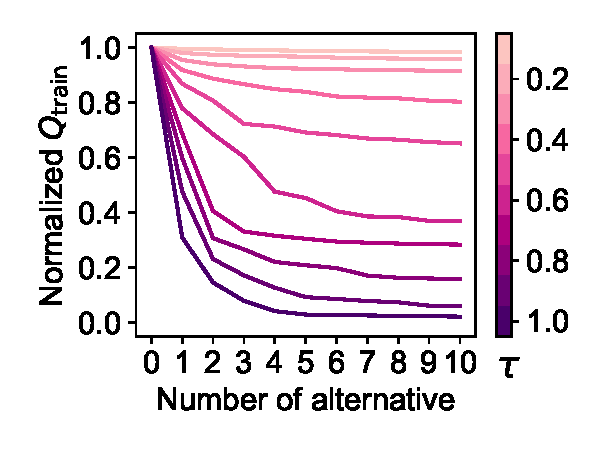
\includegraphics[width=\textwidth, trim=15 15 10 15, clip]{plots/afs-impact-num-alternatives-tau-train-objective-max-fillna.pdf}
		\caption{
			Training-set objective value, max-normalized.
			Infeasible feature sets assigned a quality of~0.
		}
		\label{fig:afs:impact-num-alternatives-tau-train-objective-max-fillna}
	\end{subfigure}
	\\ \vspace{\baselineskip}
	\begin{subfigure}[t]{0.48\textwidth}
		\centering
		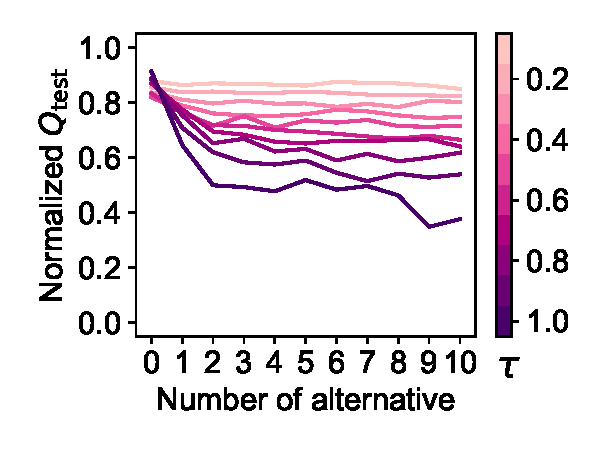
\includegraphics[width=\textwidth, trim=15 15 10 15, clip]{plots/afs-impact-num-alternatives-tau-test-objective-max.pdf}
		\caption{
			Test-set objective value, max-norma\-lized.
			Infeasible feature sets excluded.
		}
		\label{fig:afs:impact-num-alternatives-tau-test-objective-max}
	\end{subfigure}
	\hfill
	\begin{subfigure}[t]{0.48\textwidth}
		\centering
		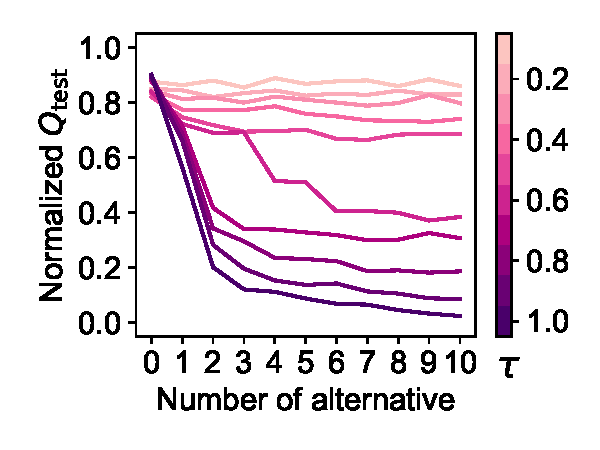
\includegraphics[width=\textwidth, trim=15 15 10 15, clip]{plots/afs-impact-num-alternatives-tau-test-objective-max-fillna.pdf}
		\caption{
			Test-set objective value, max-norma\-lized.
			Infeasible feature sets assigned a quality of~0.
		}
		\label{fig:afs:impact-num-alternatives-tau-test-objective-max-fillna}
	\end{subfigure}
	\\ \vspace{\baselineskip}
	\begin{subfigure}[t]{0.48\textwidth}
		\centering
		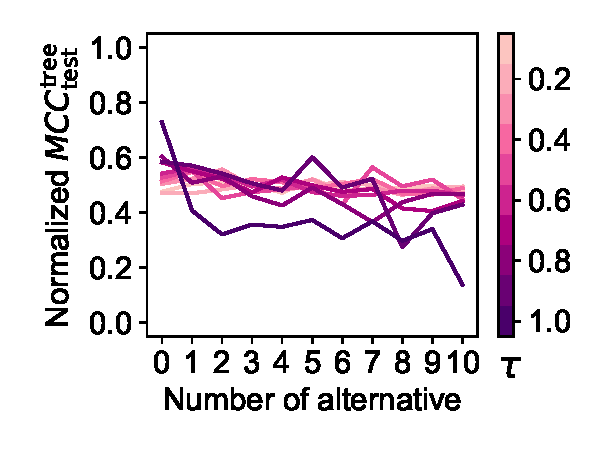
\includegraphics[width=\textwidth, trim=15 15 10 15, clip]{plots/afs-impact-num-alternatives-tau-decision-tree-test-mcc-min-max.pdf}
		\caption{
			Test set prediction performance, min-max-normalized.
			Infeasible feature sets excluded.
		}
		\label{fig:afs:impact-num-alternatives-tau-decision-tree-test-mcc-min-max}
	\end{subfigure}
	\hfill
	\begin{subfigure}[t]{0.48\textwidth}
		\centering
		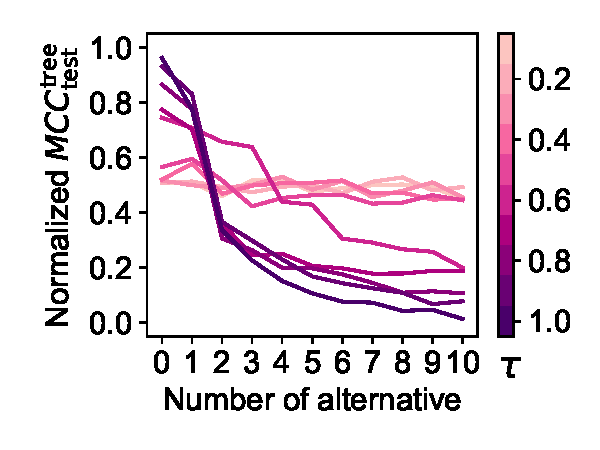
\includegraphics[width=\textwidth, trim=15 15 10 15, clip]{plots/afs-impact-num-alternatives-tau-decision-tree-test-mcc-min-max-fillna.pdf}
		\caption{
			Test set prediction performance, min-max-normalized.
			Infeasible feature sets assigned a quality of~0.
		}
		\label{fig:afs:impact-num-alternatives-tau-decision-tree-test-mcc-min-max-fillna}
	\end{subfigure}
	\caption{
		Mean of feature-set quality, normalized per experimental setting, over the number of alternatives and dissimilarity threshold~$\tau$, by evaluation metric.
		Results from sequential search with \emph{MI} as feature-selection method and $k=10$.
	}
	\label{fig:afs:impact-num-alternatives-tau-quality}
\end{figure}

\paragraph{Feature-set quality}

As Figure~\ref{fig:afs:impact-num-alternatives-tau-train-objective-max} shows for \emph{MI} as feature-selection method, the decrease of the objective value~$Q$ over the number of alternatives strongly depends on the dissimilarity threshold~$\tau$.
Note that we use results from $k=10$ instead of $k=5$ here to show more distinct values of $\tau$.
For a low dissimilarity threshold, e.g., $\tau=0.1$, the objective value barely drops over the number of alternatives.
In contrast, the objective value decreases significantly for a high dissimilarity threshold, e.g., $\tau=1$.
This is expected, since a higher~$\tau$ constrains the feature selection more by preventing the selection of previously selected features more strongly.
As Figure~\ref{fig:afs:impact-num-alternatives-tau-test-objective-max} displays, this phenomenon also holds for the test-set objective value, though the dependency on~$\tau$ is less prominent there.
In contrast, the effect of~$\tau$ on prediction performance exhibits a less clear trend, as visualized in Figure~\ref{fig:afs:impact-num-alternatives-tau-decision-tree-test-mcc-min-max}.
This result underlines our previous observation that the objective value is only partially indicate of prediction performance.

\begin{figure}[htbp]
	\centering
	\begin{subfigure}[t]{0.48\textwidth}
		\centering
		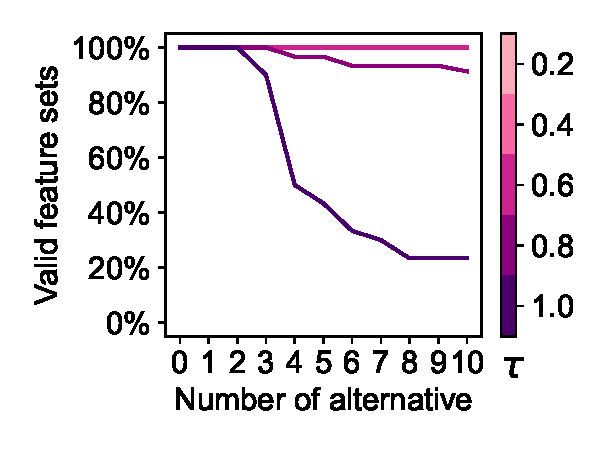
\includegraphics[width=\textwidth, trim=15 15 10 15, clip]{plots/afs-impact-num-alternatives-tau-optimization-status-k-5.pdf}
		\caption{Feature-set size~$k=5$.}
		\label{fig:afs:impact-num-alternatives-tau-optimization-status-k-5}
	\end{subfigure}
	\hfill
	\begin{subfigure}[t]{0.48\textwidth}
		\centering
		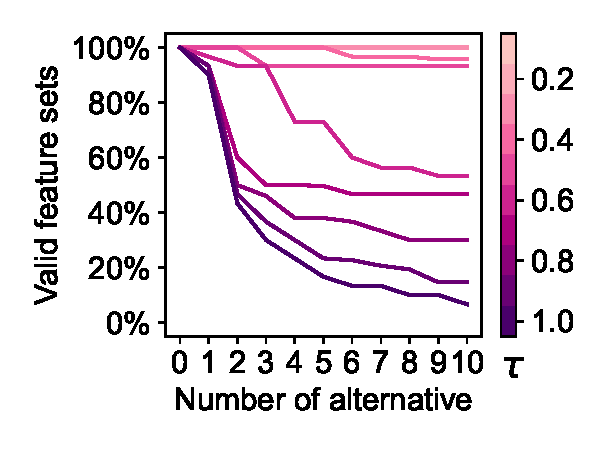
\includegraphics[width=\textwidth, trim=15 15 10 15, clip]{plots/afs-impact-num-alternatives-tau-optimization-status-k-10.pdf}
		\caption{Feature-set size~$k=10$.}
		\label{fig:afs:impact-num-alternatives-tau-optimization-status-k-10}
	\end{subfigure}
	\caption{
		Fraction of optimization runs yielding a valid feature set over the number of alternatives and dissimilarity threshold~$\tau$.
		Results from sequential search with \emph{MI} as feature-selection method.
	}
	\label{fig:afs:impact-num-alternatives-tau-optimization-status}
\end{figure}

\paragraph{Optimization status}

Similar to our previous analysis for the number of alternatives in Section~\ref{sec:afs:evaluation:search:num-alternatives}, one also needs to consider that setting~$\tau$ to certain values can make the optimization problem infeasible.
In particular, for a higher dissimilarity threshold, the likelihood is higher that there is no feature set that is alternative enough.
Figure~\ref{fig:afs:impact-num-alternatives-tau-optimization-status} visualizes how the fraction of valid feature sets develops over the number of alternatives and dissimilarity threshold~$\tau$.
Figures~\ref{fig:afs:impact-num-alternatives-tau-train-objective-max-fillna},~\ref{fig:afs:impact-num-alternatives-tau-test-objective-max-fillna}, and~\ref{fig:afs:impact-num-alternatives-tau-decision-tree-test-mcc-min-max-fillna} account for infeasible feature sets by setting their feature-set quality to zero.
Compared to Figures~\ref{fig:afs:impact-num-alternatives-tau-train-objective-max},~\ref{fig:afs:impact-num-alternatives-tau-test-objective-max}, and~\ref{fig:afs:impact-num-alternatives-tau-decision-tree-test-mcc-min-max}, the decrease in objective value is noticeably stronger.
In contrast, if only considering valid feature sets, the mean objective value can increase over the number of alternatives, as visible in Figure~\ref{fig:afs:impact-num-alternatives-tau-train-objective-max} for $\tau=1.0$ or in Figure~\ref{fig:afs:impact-num-alternatives-fs-method-train-objective-max} for \emph{MI} and \emph{Model Gain}.
This counterintuitive phenomenon can occur because some datasets run out of valid feature sets sooner than others, so the average quality is determined for different sets of datasets at each number of alternatives.

\begin{figure}[htbp]
	\centering
	\begin{subfigure}[t]{0.48\textwidth}
		\centering
		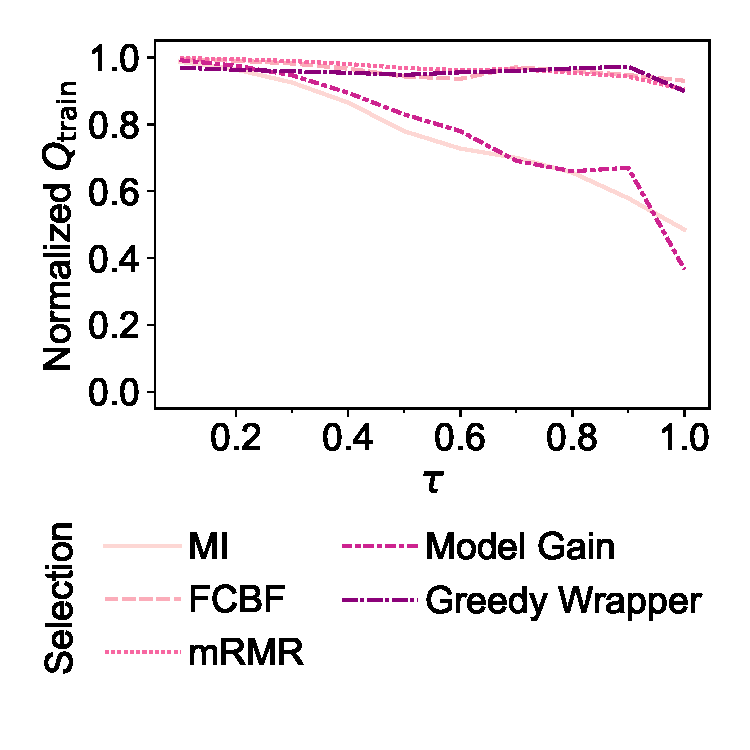
\includegraphics[width=\textwidth, trim=20 40 15 15, clip]{plots/afs-impact-tau-fs-method-train-objective-max.pdf}
		\caption{
			Training-set objective value.
			Infeasible feature sets excluded.
		}
		\label{fig:afs:impact-tau-fs-method-train-objective-max}
	\end{subfigure}
	\hfill
	\begin{subfigure}[t]{0.48\textwidth}
		\centering
		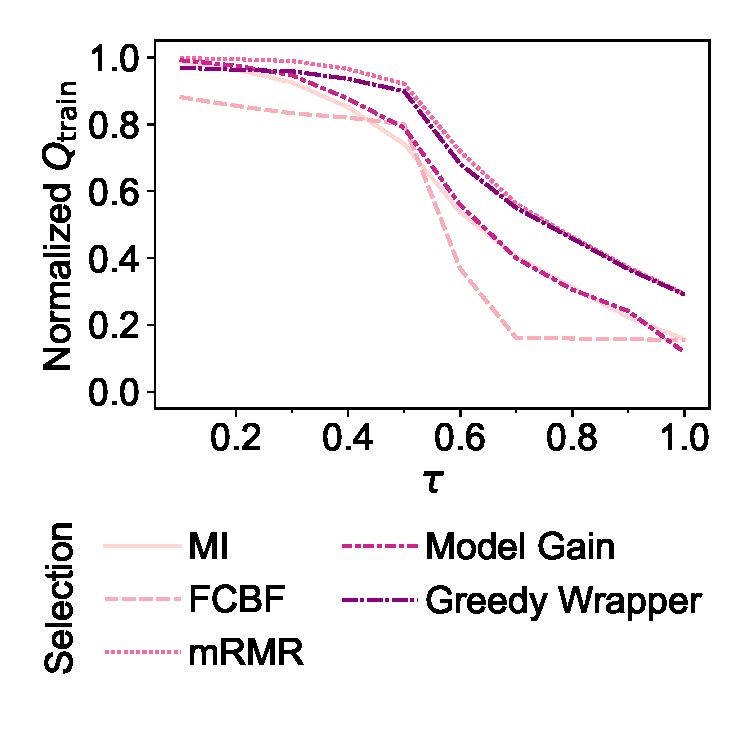
\includegraphics[width=\textwidth, trim=20 40 15 15, clip]{plots/afs-impact-tau-fs-method-train-objective-max-fillna.pdf}
		\caption{
			Training-set objective value.
			Infeasible feature sets assigned a quality of~0.
		}
		\label{fig:afs:impact-tau-fs-method-train-objective-max-fillna}
	\end{subfigure}
	\\ \vspace{\baselineskip}
	\begin{subfigure}[t]{0.48\textwidth}
		\centering
		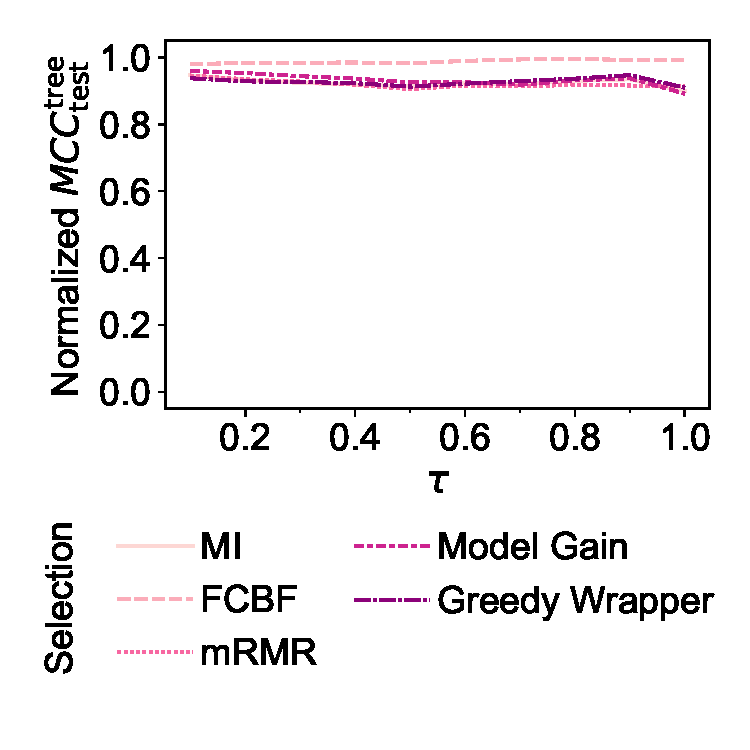
\includegraphics[width=\textwidth, trim=20 40 15 15, clip]{plots/afs-impact-tau-fs-method-decision-tree-test-mcc-max.pdf}
		\caption{
			Test-set prediction performance.
			Infeasible feature sets excluded.
		}
		\label{fig:afs:impact-tau-fs-method-decision-tree-test-mcc-max}
	\end{subfigure}
	\hfill
	\begin{subfigure}[t]{0.48\textwidth}
		\centering
		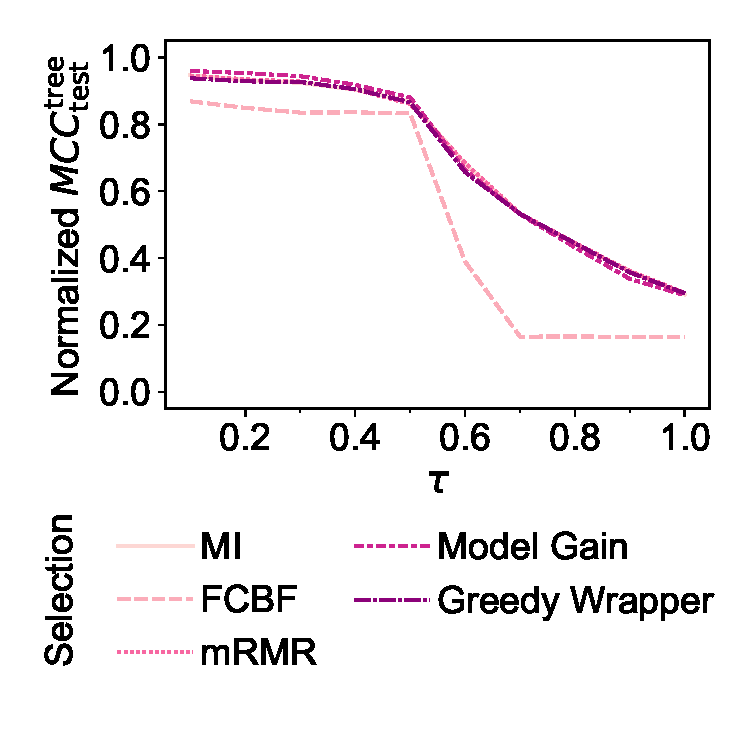
\includegraphics[width=\textwidth, trim=20 40 15 15, clip]{plots/afs-impact-tau-fs-method-decision-tree-test-mcc-max-fillna.pdf}
		\caption{
			Test-set prediction performance.
			Infeasible feature sets assigned a quality of~0.
		}
		\label{fig:afs:impact-tau-fs-method-decision-tree-test-mcc-max-fillna}
	\end{subfigure}
	\caption{
		Mean feature-set quality, max-normalized per experimental setting, over the dissimilarity threshold~$\tau$, by evaluation metric and feature-selection method.
		Results from sequential search with $k=10$.
	}
	\label{fig:afs:impact-tau-fs-method-quality}
\end{figure}

\paragraph{Influence of feature-selection method}

While the previous observations applied to \emph{MI} as feature-selection method, they do not hold universally, as Figure~\ref{fig:afs:impact-tau-fs-method-train-objective-max} shows.
Besides \emph{MI}, the objective value of \emph{Model Gain} strongly depends on~$\tau$ as well.
In contrast, the remaining three feature-selection methods exhibit less influence of~$\tau$ on the quality of found feature sets, unless one also considers infeasible feature sets (cf.~Figure~\ref{fig:afs:impact-tau-fs-method-train-objective-max-fillna}).
For \emph{Greedy Wrapper}, this outcome can be explained by the heuristic search procedure to find feature sets.
For \emph{FCBF}, the fraction of infeasible solutions is much higher than for \emph{MI} in general, so this aspect plays a larger role than the quality variation of found feature sets.
For \emph{mRMR}, the low influence of~$\tau$ matches the low influence of the number of alternatives.
For this feature-selection method, alternative feature sets seem to vary little in their objective value.

Further, the test-set prediction performance does not vary considerably over $\tau$ for any of the feature-selection methods, as Figure~\ref{fig:afs:impact-tau-fs-method-decision-tree-test-mcc-max} displays.
Only considering infeasible feature sets results in a decrease of prediction performance (cf.~Figure~\ref{fig:afs:impact-num-alternatives-tau-decision-tree-test-mcc-min-max-fillna}).

\subsection{Summary}
\label{sec:afs:evaluation:summary}

\paragraph{Datasets (cf.~Section~\ref{sec:afs:evaluation:datasets})}

Generally, feature-set quality strongly depended on the dataset.
Thus, an analysis of alternative feature sets needs be dataset-specific or appropriately normalize quality.

\paragraph{Feature-set quality metrics (cf.~Section~\ref{sec:afs:evaluation:metrics})}

Different notions of feature-set quality exhibited different patterns when we varied other experimental dimensions, so one should decide on a notion of feature-set quality carefully.
In particular, the objective function of simple feature-selection methods might disagree with actual prediction performance of the corresponding feature sets.
Further, we observed overfitting, i.e., a gap between training-set quality and test-set quality, also for simple objective functions, though to a lesser extent than for prediction performance.

\paragraph{Feature-selection methods (cf.~Section~\ref{sec:afs:evaluation:feature-selection})}

Among the feature-selection methods, \emph{Model Gain} resulted in the best prediction performance on average, though the simple univariate \emph{MI} also turned out competitive in that regard.
Further, \emph{Greedy Wrapper} and \emph{mRMR} required high optimization times, while our constrained-based version of \emph{FCBF} yielded many infeasible solutions.
Finally, selecting $k=10$ instead of $k=5$ features only yielded a small improvement for all feature-selection methods, so one might stick to smaller feature-set sizes if such a setting benefits interpretability for users.

\paragraph{Search methods for alternatives (cf.~Section~\ref{sec:afs:evaluation:search:method})}

Simultaneous search, particularly with min-aggregation, considerably reduced the variance in the training-set objective value over alternatives compared to sequential search, as we desired.
However, results were less clear on the test set and when considering prediction performance to measure feature-set quality.
Further, the average quality of alternatives was similar between the search methods.
In addition, sequential search was considerably faster than the simultaneous one and thereby led to less solver timeouts, particularly when increasing the number of alternatives.
Also, sequential search allows users to stop search after each alternative instead of requiring the number of alternatives to be determined beforehand.
Thus, we recommend using sequential search.

\paragraph{Number of alternatives $a$ (cf.~Section~\ref{sec:afs:evaluation:search:num-alternatives})}

Feature-set quality showed the highest decrease from the original feature set to the first alternative but less beyond.
The strength of this decrease depended on the feature-selection method.
There usually were several alternatives of similar quality if such valid alternatives existed at all.
In particular, the frequency of infeasible solutions naturally increased with~$a$ due to the presence of more constraints.
Finally, the quality decrease was more prominent on the training set than on the test set.

\paragraph{Dissimilarity threshold $\tau$ (cf.~Section~\ref{sec:afs:evaluation:search:tau})}

As expectable, a higher dissimilarity threshold caused a stronger decrease of feature-set quality in terms of objective value for the feature-selection methods \emph{MI} and \emph{Model Gain}.
This result shows that users can control a trade-off between quality and dissimilarity, making a use-case-specific decision.
However, results regarding prediction performance and for the other three feature-selection methods were less clear.
In any case, a higher~$\tau$ naturally caused more infeasible solutions, which users should be aware of.

\section{Conclusions and Future Work}
\label{sec:afs:conclusion}

In this section, we summarize our work (cf.~Section~\ref{sec:afs:conclusion:conclusion}) and give an outlook on potential future work (cf.~Section~\ref{sec:afs:conclusion:future-work}).

\subsection{Conclusions}
\label{sec:afs:conclusion:conclusion}

Feature-selection methods are a valuable tool to foster interpretable predictions.
Conventional feature-selection methods typically yield only one feature set.
However, users may be interested in obtaining multiple, sufficiently diverse feature sets that also have high quality.
Such alternative feature sets may provide alternative explanations for predictions from the data.

In this article, we defined alternative feature selection as an optimization problem.
We formalized alternatives via constraints that are independent of the feature-selection method, can be combined with other constraints on feature sets, and allow users to control diversity according to their needs.
We analyzed the complexity of this optimization problem and proofed $\mathcal{NP}$-hardness, even for simple notions of feature-set quality.
Further, we discussed how to integrate different categories of conventional feature-selection methods.
Finally, we evaluated alternative feature selection with 30 classification datasets and five feature-selection methods.
We compared two search methods for alternatives and varied the number of alternatives as well as the threshold for alternatives.

\subsection{Future Work}
\label{sec:afs:conclusion:future-work}

\paragraph{Feature selection (objective function)}

One could search for alternatives with other feature-selection methods than the five we analyzed.
For wrapper feature selection, which requires black-box optimization, we implemented only one of several ways to consider alternatives (cf.~Section~\ref{sec:afs:approach:objectives:black-box}).
As our experiments showed, the runtime poses a particular challenge for this category of feature selection.
Further, our search procedures for alternatives would need adaptation to also work for embedded feature selection (cf.~Section~\ref{sec:afs:approach:objectives:embedding}).

\paragraph{Alternatives (constraints)}

One could vary the definition of alternatives (cf.~Sections~\ref{sec:afs:approach:problem} and~\ref{sec:afs:approach:constraints}), e.g., the set-dissimilarity measure, the definitions for multiple alternatives, or by using soft constraints instead of hard constraints.
While we made general and straightforward decisions for each of these points, particular applications might demand other formalizations of alternatives.

\paragraph{Computational complexity} Appendix~\ref{sec:afs:appendix:complexity:future} discuses how one could extend our complexity analysis of alternative feature selection (cf.~Section~\ref{sec:afs:approach:complexity}).

\paragraph{Simultaneous search}

Our experiments (cf.~Section~\ref{sec:afs:evaluation:search:method}) and theoretical analyses (cf.~Section~\ref{sec:afs:approach:constraints:multiple}) revealed that simultaneous search scales badly with the number of alternatives.
One could try to find a more efficient problem formulation, e.g., by loosening the constraints for alternatives, which could bear the danger of allowing identical feature sets as alternatives.
Further, one could limit the solver runtime and take the intermediate results once the timeout is reached.
We already used a fixed timeout in our experiments, but studying the exact influence of timeouts one the feature-set quality is a topic for future work.
Next, one could use a different solver, e.g., one that supports non-linear terms so the auxiliary variables from Equation~\ref{eq:afs:product-linear} become superfluous.
Finally, one could develop a heuristic rather than an exact search procedure (cf.~Appendix~\ref{sec:afs:appendix:univariate-search-algorithm}).

\paragraph{Datasets}

Our evaluation uses datasets from various domains.
While we could uncover several general trends, the existence and the quality of alternatives clearly depends on the dataset (cf.~Section~\ref{sec:afs:evaluation:datasets}).
Thus, practitioners could use our generic search methods for alternatives in domain-specific case studies.

\appendix

\section{Appendix}
\label{sec:afs:appendix}

In this section, we provide technical details and discuss approaches not used in our experiments.
Section~\ref{sec:afs:appendix:simultaneous-objective-aggregation} discusses aggregation operators for the objective of simultaneous search (cf.~Equation~\ref{eq:afs:afs-simultaneous}).
Section~\ref{sec:afs:appendix:multivariate-filter-objectives} discusses further objective functions for multivariate filter feature selection, amending Section~\ref{sec:afs:approach:objectives:white-box}.
Section~\ref{sec:afs:appendix:complete-optimization-problem} provides complete definitions of the alternative-feature-selection problem, which we described over the course of Section~\ref{sec:afs:approach}.
Section~\ref{sec:afs:appendix:complexity} amends the complexity analysis from Section\ref{sec:afs:approach:complexity}.
Section~\ref{sec:afs:appendix:univariate-search-algorithm} presents a greedy heuristic for univariate feature selection (cf.~Equation~\ref{eq:afs:univariate-filter}).

\subsection{Aggregation Operators for Simultaneous Search}
\label{sec:afs:appendix:simultaneous-objective-aggregation}

In this section, we discuss operators to aggregate feature-set quality of multiple alternatives in the objective of simultaneous search (cf.~Equation~\ref{eq:afs:afs-simultaneous}).

\paragraph{Sum-aggregation}

The arguably simplest way to aggregate the qualities of multiple feature sets is to sum them up, which we call \emph{sum-aggregation}:
%
\begin{equation}
	\max_{s^{(0)}, \dots, s^{(a)}} \sum_{i=0}^a Q(s^{(i)},X,y)
	\label{eq:afs:afs-simultaneous-sum-objective}
\end{equation}
%
While this objective fosters a high average quality of feature sets, it does not guarantee that the alternatives have similar quality:
%
\begin{example}
Consider univariate filter feature selection (cf.~Equation~\ref{eq:afs:univariate-filter}) with $n=6$~features, feature qualities~$q = (9,8,7,3,2,1)$, feature-set size~$k=3$, number of alternatives~$a=2$, and dissimilarity threshold~$\tau = 0.5$, which permits an overlap of one feature between sets here.
Sequential search yields the selection $s^{(0)} = (1,1,1,0,0,0)$, $s^{(1)} = (1,0,0,1,1,0)$, and $s^{(2)} = (0,1,0,1,0,1)$, with a summed quality of $24+14+12=50$.
One simultaneous-search solution consists of the feature sets $s^{(0)} = (1,1,0,1,0,0)$, $s^{(1)} = (1,0,1,0,1,0)$, and $s^{(2)} = (0,1,1,0,0,1)$, with a summed quality of $20+18+16=54$.
Another simultaneous-search solution is $s^{(0)} = (1,1,0,0,0,1)$, $s^{(1)} = (1,0,1,0,1,0)$, and $s^{(2)} = (0,1,1,1,0,0)$, with a summed quality of $18+18+18=54$.
\end{example}
%
This example allows several insights.
First, sequential search yields worse quality than simultaneous search here, i.e., 50 vs.~54.
Second, the feature-set qualities of the sequential solution, i.e., 24, 14, and~12, differ significantly.
Third, simultaneous search can yield multiple solutions whose feature-set quality is differently balanced.
Here, the feature-set qualities in the second simultaneous-search solution, i.e., 18, 18, and~18, are more balanced than in the first one, i.e., 20, 18, and~16.
However, both solutions are equally optimal for sum-aggregation.

\paragraph{Min-aggregation}

To actively foster balanced feature-set qualities in simultaneous search, we propose \emph{min-aggregation}:
%
\begin{equation}
	\max_{s^{(0)}, \dots, s^{(a)}} \min_{i \in \{0, \dots, a\}} Q(s^{(i)},X,y) \\
	\label{eq:afs:afs-simultaneous-min-objective}
\end{equation}
%
In the terms of social choice theory, this objective uses an egalitarian rule instead of a utilitarian one~\cite{myerson1981utilitarianism}.
Note that optimizing the objective with either sum-aggregation or min-aggregation does not necessarily optimize the other one.
We already showed an example for a solution optimizing sum-aggregation but not min-aggregation.
In the following, we demonstrate the other direction:
%
\begin{example}
Consider univariate filter feature selection (cf.~Equation~\ref{eq:afs:univariate-filter}) with $n=6$~features, feature qualities~$q = (11,10,6,5,4,1)$, feature-set size~$k=3$, number of alternatives~$a=1$, and dissimilarity threshold~$\tau = 0.5$, which permits an overlap of one feature between sets here.
One solution optimizing the objective with min-aggregation is $s^{(0)} = (1,1,0,0,1,0)$ and $s^{(1)} = (1,0,1,1,0,0)$, with a summed quality of $25+22=47$.
Another solution is $s^{(0)} = (1,1,0,0,0,1)$ and $s^{(1)} = (1,0,1,1,0,0)$, with a summed quality of $22+22=44$.
\end{example}
%
While both solutions have the same minimum quality, only the first solution optimizes the objective with sum-aggregation.
In particular, min-aggregation allows reducing the quality of sets that are above the minimum of all sets.

From the technical perspective, Equation~\ref{eq:afs:afs-simultaneous-min-objective} has the disadvantage of being non-linear regarding the decision variables $s^{(0)}, \dots, s^{(a)}$.
However, we can linearize it with one constraint per feature set and an auxiliary variable~$Q_{\text{min}}$:
%
\begin{equation}
	\begin{aligned}
		\max_{s^{(0)}, \dots, s^{(a)}} &\quad &Q_{\text{min}} & \\
		\text{subject to:} &\quad \forall i \in \{0, \dots, a\}: &Q_{\text{min}} &\leq Q(s^{(i)},X,y) \\
		&\quad & Q_{\text{min}} &\in \mathbb{R}
	\end{aligned}
	\label{eq:afs:afs-simultaneous-min-objective-linear}
\end{equation}
%
As we maximize~$Q_{\text{min}}$, this variable will implicitly assume the actual minimum value of~$Q(s^{(i)},X,y)$ with equality since the solution would not be optimal otherwise.
This situation relieves us from introducing further auxiliary variables that are usually necessary when linearizing maximum or minimum expressions~\cite{mosek2022modeling}.

\paragraph{Further approaches for balancing quality}

Min-aggregation provides no control or guarantee how much the feature-set qualities will actually differ between alternatives since it only incentives high quality for all sets.
One can alleviate this issue by adapting the objective and/or constraints.
First, work on number partitioning also use other objectives for balancing~\cite{korf2010objective, lawrinenko2017identical} (cf.~Section~\ref{sec:afs:approach:complexity:uni-min-partitioning}).
E.g., one could minimize the difference between maximum and minimum feature-set quality.
Second, one could use sum-aggregation but constrain the minimum or maximum quality of sets, or the difference between the qualities.
However, such constraint-based approaches introduce one or several parameters bounding feature-set quality, which are difficult to determine a priori.
Third, one could consider balancing qualities as another objective besides the maximizing the summed quality.
One can then optimize two objectives simultaneously, filtering results for Pareto-optimal solutions, or optimize a weighted combination of the two objectives.
In both cases, users may need to define an acceptable trade-off between the two objectives.
It is an open question if always one solution exists that jointly optimizes min- and sum-aggregation.
If yes, then optimizing a weighted combination of the two objectives would also optimize each of them on its own, assuming positive weights.

\subsection{Further Objectives for Multivariate Filter Methods}
\label{sec:afs:appendix:multivariate-filter-objectives}

While Section~\ref{sec:afs:approach:objectives:white-box} already addressed FCBF and mRMR as multivariate filter feature-selection methods, we discuss the objectives of CFS and Relief here.

\paragraph{CFS}

Correlation-based Feature Selection (CFS)~\cite{hall1999correlation, hall2000correlation} follows a similar principle as mRMR but uses the ratio instead of the difference between a relevance term and a redundancy term for feature-set quality.
Using a bivariate dependency measure $q(\cdot)$ to quantify correlation, the objective is as follows:
%
\begin{equation}
	Q_{\text{CFS}}(s,X,y) = \frac{\sum_{j=1}^{n} q(X_{\cdot{}j},y) \cdot s_j}{\sqrt{\sum_{j=1}^{n} s_j + \sum_{j_1=1}^{n} \sum_{\substack{j_2=1 \\ j_2 \neq j_1}}^{n} q(X_{\cdot{}j_1}, X_{\cdot{}j_2}) \cdot s_{j_1} \cdot s_{j_2}}}
	\label{eq:afs:cfs}
\end{equation}
%
One can square this objective to remove the square root in the denominator~\cite{nguyen2010towards}.
Nevertheless, the objective remains non-linear in the decision variables~$s$ since it involves a fraction and multiplications between variables.
However, one can linearize the objective with additional variables and constraints~\cite{nguyen2010improving, nguyen2010towards}, allowing to formulate alternative feature selection as a linear problem.

\paragraph{Relief}

Relief~\cite{kira1992feature, robnik1997adaptation} builds on the idea that data objects with a similar value of the prediction target should have similar feature values, but data objects that differ in their target should differ in their feature values.
Relief assigns a score to each feature by sampling data objects and quantifying the difference in feature values and target values compared to their nearest neighbors.
We deem Relief to be multivariate since the nearest-neighbor computations involve all features instead of considering them independently.
However, the resulting feature scores can directly be put into the univariate-filter objective (cf.~Equation~\ref{eq:afs:univariate-filter}) to obtain a linear problem.
One can also use Relief scores in CFS to consider feature redundancy~\cite{hall1999correlation, hall2000correlation}, which the default Relief does not.

\subsection{Complete Specifications of the Optimization Problem}
\label{sec:afs:appendix:complete-optimization-problem}

In this section, we provide complete specifications of the alternative-feature-selection problem for sequential and simultaneous search.
In particular, we combine all relevant definitions and equations from Section~\ref{sec:afs:approach}.
We use the objective of univariate filter feature selection (cf.~Equation~\ref{eq:afs:univariate-filter}).
The corresponding feature qualities $q(\cdot)$ are constants in the optimization problem.
We use the Dice dissimilarity (cf.~Equation~\ref{eq:afs:dice-rearranged-equal-size}) to measure feature-set dissimilarity for alternatives.
The dissimilarity threshold~$\tau \in [0,1]$ is a user-defined constant.
Further, we assume fixed, user-defined feature-set sizes~$k \in \mathbb{N}$.

\paragraph{Sequential alternatives}

In the sequential case, only one feature set~$F_s$ is variable in the optimization problem, while the existing feature sets $F_{\bar{s}} \in \mathbb{F}$ with their selection vectors $\bar{s}$ are constants.
%
\begin{equation}
	\begin{aligned}
		\max_s &\quad & Q_{\text{uni}}(s,X,y) &= \sum_{j=1}^{n} q(X_{\cdot{}j},y) \cdot s_j \\
		\text{subject to:} &\quad \forall F_{\bar{s}} \in \mathbb{F}: & \sum_{j=1}^n s_j \cdot \bar{s}_j &\leq (1 - \tau) \cdot k \\
		&\quad & \sum_{j=1}^n s_j &= k \\
		&\quad & s &\in \{0,1\}^n
	\end{aligned}
	\label{eq:afs:afs-sequential-complete}
\end{equation}
%
\paragraph{Simultaneous alternatives}

In the simultaneous case, all feature sets are variable.
$a \in \mathbb{N}$ denotes the number of alternatives, which corresponds to the number of feature sets minus one.
Next, we introduce auxiliary variables according to linearize products between variables (cf.~Equation~\ref{eq:afs:product-linear}).
Finally, we use sum-aggregation (cf.~Equation~\ref{eq:afs:afs-simultaneous-sum-objective}) in the objective here.
%
\begin{equation}
	\begin{aligned}
		\max_{s^{(0)}, \dots, s^{(a)}} &\quad & \sum_i Q_{\text{uni}}(s^{(i)},X,y) &= \sum_i \sum_j q(X_{\cdot{}j},y) \cdot s^{(i)}_j\\
		\text{subject to:} &\quad \forall i_1~\forall i_2: & \sum_j t^{(i_1,i_2)}_j &\leq (1 - \tau) \cdot k \\
		&\quad \forall i_1~\forall i_2~\forall j: & t^{(i_1,i_2)}_j &\leq s^{(i_1)}_j \\
		&\quad \forall i_1~\forall i_2~\forall j: & t^{(i_1,i_2)}_j &\leq s^{(i_2)}_j \\
		&\quad \forall i_1~\forall i_2~\forall j: & 1 + t^{(i_1,i_2)}_j &\geq s^{(i_1)}_j + s^{(i_2)}_j \\
		&\quad \forall i: & \sum_j s^{(i)}_j &= k \\
		&\quad \forall i: & s^{(i)} &\in \{0,1\}^n \\
		&\quad \forall i_1~\forall i_2: & t^{(i_1,i_2)} &\in \{0,1\}^n \\
		\text{with indices:} &\quad & i &\in \{0, \dots, a\} \\
		&\quad & i_1 &\in \{1, \dots, a\} \\
		&\quad & i_2 &\in \{0, \dots, i_1-1\} \\
		&\quad & j &\in \{1, \dots, n\}
	\end{aligned}
	\label{eq:afs:afs-simultaneous-complete}
\end{equation}

\subsection{Computational Complexity}
\label{sec:afs:appendix:complexity}

In this section, we provide further details for the computational complexity of alternative feature selection (cf.~Section~\ref{sec:afs:approach:complexity}).
In particular, we outline future work (cf.~Section~\ref{sec:afs:appendix:complexity:future}).

\subsubsection{Future Work}
\label{sec:afs:appendix:complexity:future}

\paragraph{Scenarios of alternative feature selection}

Our prior complexity analyses focused on special cases of alternative feature selection, while other cases might be interesting as well.
For example, though we obtained $\mathcal{NP}$-hardness for min-aggregation with feature-set overlap (cf.~Proposition~\ref{prop:afs:complexity-no-partitioning-min-constrained-k}), an analysis of sum-aggregation with overlap is open, even for sequential search, i.e., just optimizing one alternative at once.
While sum-aggregation admits polynomial runtime subject to $\tau=1$ (cf.~Proposition~\ref{prop:afs:complexity-partitioning-sum}), this result might not extend to~$\tau < 1$.
In particular, $\tau < 1$ increases the number of valid solutions, which could negatively affect the runtime for searching the optimum.

Further, our complexity analyses mostly assumed univariate feature qualities.
Other feature-selection methods have different objective functions and can therefore reside in different complexity classes.
In particular, many other objective functions are more sophisticated and thereby harder to evaluate.

\paragraph{Complexity classes}

For analyzing further cases of alternative feature selection, several questions spring to mind.
As a first step, one could establish a general complexity result like $\mathcal{NP}$-hardness or the existence of a polynomial-time algorithm.
In the former case, it is interesting to know whether there are at least pseudo-polynomial exact approaches or (fully) polynomial-time approximation schemes.
Further, there might be efficient algorithms for problem instances satisfying additional requirements.
Finally, while we placed alternative feature selection in the broad parameterized complexity class~$\mathcal{XP}$, one might proof either membership or hardness for more specific parameterized classes.

\paragraph{Related problem formulations}

We only focused on the optimization problem of alternative feature selection until now.
Another interesting question is how many alternatives, regardless of their quality, can be found for a given $n$, $k$, and $\tau$.
Also, given the number of alternatives as well, it would be interesting to have an exact or approximate estimate for the number of valid solutions for alternative feature selection, i.e., sets of feature sets.
While both these estimates are straightforward for $\tau = 1$, allowing arbitrary~$\tau$ poses a larger challenge.

Further, one could re-formulate alternative feature selection similar to the \textsc{Bin Covering} problem.
\textsc{Bin Covering}~\cite{assmann1984dual} distributes elements with individual weights into bins such that the number of bins is maximal and the summed weights in each bin surpass certain limit.
In related work, \cite{lawrinenko2017identical} noted a connection between \textsc{Multi-Way Number Partitioning} and \textsc{Bin Covering}.
This relationship can help develop better solution approaches for either problem~\cite{walter2017lower, walter2017improved}.
In our case, we could ask to maximize the number of alternatives such that each feature set's quality exceeds a user-defined threshold.
This particular problem formulation assumes univariate qualities and $\tau=1$ again.

\subsection{Finding Alternatives for Univariate Feature Qualities}
\label{sec:afs:appendix:univariate-search-algorithm}

For an objective consisting of univariate feature qualities (cf.~Equation~\ref{eq:afs:univariate-filter} and Section~\ref{sec:afs:appendix:complete-optimization-problem}), one can easily find a limited number of optimal alternative feature sets without a solver.
To this end, we propose the following \emph{greedy-replacement} procedure, displayed in Algorithm~\ref{al:afs:greedy-replacement}:

TODO: use proof-sketch environment in complexity part
TODO: can adapt this procedure to min-quality objective, potentially using number partitioning heuristics (have a look at the latter!) (e.g., always select features of highest quality, bring the rest in some (sorted?) order and sequentially assign to set with currently lowest sum)
TODO: think if sequential search can act as bound for simultaneous search
TODO: think if PTAS / APX can be shown
- relaxation also gives an bound on objective (though no solution) but might be very loose
- if you can use the top features and there are still unused features, you have at least a certain approximation ratio (depending on how large the quality of the top (1-tau)*k features is relative to the top k features -> poly-apx or even apx, depending on whether you consider k fixed)

\paragraph{Procedure}

The univariate objective function does not contain interaction terms between features.
Thus, we start by sorting the features decreasingly according to their individual qualities~$q_j$.
Given a desired feature-set size~$k$, the optimal original feature set, i.e., the zeroth alternative, simply consists of the first~$k$ features from this quality-based ordering.
Depending on the set-dissimilarity measure defining alternatives, one can then determine how many features needs to differ for obtaining a valid alternative.
For the Dice dissimilarity we use in our article, including Algorithm~\ref{al:afs:greedy-replacement}, $\lceil \tau \cdot k \rceil$~features need to differ between feature sets (cf.~Equation~\ref{eq:afs:dice-rearranged-equal-size}).
Consequently, a fixed subset of $\lfloor (1 - \tau) \cdot k \rfloor$~features can be contained in all alternatives without violating the dissimilarity threshold.
Thus, for each alternative, we always select the best $\lfloor (1 - \tau) \cdot k \rfloor$~features regarding quality~$q_j$.
We only replace the remaining $\lceil \tau \cdot k \rceil$~features from alternative to alternative.
To this end, we fill up the feature sets with the highest-quality features that were not part of any feature set yet, which ensures a sufficient pairwise dissimilarity between feature sets.
We continue this procedure till we reach the desired number of alternatives or till there are not enough unused features to form further alternatives.

\begin{algorithm}[htb]
	\DontPrintSemicolon
	\KwIn{Univariate feature qualities~$q_j$ with $j \in \{1, \dots, n\}$, \newline
		Feature-set size~$k$, \newline
		Number of alternatives~$a$, \newline
		Dissimilarity threshold~$\tau$}
	\KwOut{Feature-selection decision vectors~$s^{(\cdot)}$}
	\BlankLine
	\If(\tcp*[f]{Not enough features for selection}){$k > n$}{
		\Return{$\emptyset$}
	}
	$indices \leftarrow$ sort\_indices($q$, order=descending) \tcp*{Order by qualities}
	$s \leftarrow \{0\}^n$ \tcp*{Initial selection for all alternatives}
	$position \leftarrow 1$ \tcp*{Index of index of currently selected feature}
	\While{$position \leq \lfloor (1 - \tau) \cdot k \rfloor$}{
		$j \leftarrow indices[position]$\;
		$s_j \leftarrow 1$ \;
		$position \leftarrow position + 1$\;
	}
	$i \leftarrow 0$\ \tcp*{Number of current alternative}
	\While{$i \leq a$ \textbf{and} $i \leq \frac{n - k}{\lceil \tau \cdot k \rceil}$}{
		$s^{(i)} \leftarrow s$ \tcp*{Select best $\lfloor (1 - \tau) \cdot k \rfloor$ features}
		\For(\tcp*[f]{Select remaining $\lceil \tau \cdot k \rceil$ features}){$\_ \leftarrow 1$ \KwTo $\lceil \tau \cdot k \rceil$}{
			$j \leftarrow indices[position]$\;
			$s^{(i)}_j \leftarrow 1$\;
			$position \leftarrow position + 1$\;
		}
		$i \leftarrow i + 1$\;
	}
	\Return{$s^{(0)}, \dots, s^{(i)}$}
	\caption{Greedy-replacement search for alternative feature sets based on Dice dissimilarity.}
	\label{al:afs:greedy-replacement}
\end{algorithm}

\paragraph{Example}

With $n=10$ features, feature-set size~$k=5$, and $\tau=0.4$, each feature set has to differ by two features from the other feature sets.
The original feature set consists of the five best features regarding quality~$q(\cdot)$.
The first alternative consists of the three best features plus the sixth- and seventh-best feature.
The second alternative consists of the three best features plus the eight- and ninth-best feature.
After that alternative, the greedy-replacement procedure has to stop, as there are not enough unused features to form further alternatives.
In general, the $\lfloor (1 - \tau) \cdot k \rfloor$~best features plus the $k + (i-1) \cdot \lceil \tau \cdot k \rceil + 1$ to $k + i \cdot \lceil \tau \cdot k \rceil$~best features form the $i$-th alternative.

\paragraph{Supporting variable $k$}

One can also adapt this procedure to permit varying feature-set sizes~$k^{(i)}$ over alternatives rather than using a constant~$k$.
Especially, if one knows the values of all~$k^{(i)}$ beforehand, one can still compute the admissible overlap of feature sets (cf.~Equation~\ref{eq:afs:dice-rearranged}) and thereby determine the number of features to be replaced per iteration.
However, if the order of the $k^{(i)}$-values is flexible, the situation becomes more involved.
In particular, assembling feature sets of different sizes in different order can result in a different overall objective value, i.e., summed feature-set quality.

\paragraph{Limitations}

For a fixed~$k$, not even a simultaneous search can surpass the summed quality of the solutions yielded by the sequential greedy-replacement procedure, though the former might compose the feature sets differently.

TODO: that's wrong, see 2023-01-18 and 2022-05-23 thoughts; even with unused features available, greedy replacement can be worse than both sequential and simultaneous search (add an example with qualities 1-9, k =3, tau = 1, a = 2, as shown to Matthias)

However, greedy replacement only works as long as some features have not been part of any feature set yet, i.e., $k + i \cdot \lceil \tau \cdot k \rceil \leq n$.
Once this pool of unused features is exhausted, one would need another strategy to find further alternatives.
Additionally, continuing search from the results of greedy replacement might then perform worse than a simultaneous search.
Thus, to obtain a high number of alternatives with greedy replacement, the following conditions are beneficial:
The number of features~$n$ should be high, the feature-set size~$k$ show be low, and the dissimilarity threshold~$\tau$ should be low.
These conditions align well with conventional feature-selection scenarios where~$k \ll n$.

Besides the drawback of potentially running out of unused features, there are further disadvantages of greedy replacement compared to solver-based optimization.
In particular, greedy replacement does not work once the optimization problem gets more involved.
For example, there might be further constraints on feature sets, e.g., based on domain knowledge, which are not accounted for in Algorithm~\ref{al:afs:greedy-replacement}.
Also, the objective function becomes more complex for other feature-selection methods than univariate filters, which makes the quality-based feature ordering impossible or suboptimal.
At most, one could start with the original feature set from a sophisticated feature-selection method and then continue with greedy replacement based on univariate qualities.
Simultaneous search with min-aggregation (cf.~Equation~\ref{eq:afs:afs-simultaneous-min-objective}) also is unsuitable for greedy replacement.

Overall, greedy replacement is a fast search procedure for special scenarios, but a solver-based search for alternatives is more general.
Our experiments in Section~\ref{sec:afs:evaluation} consistently use a solver.

\renewcommand*{\bibfont}{\small} % use a smaller font for bib than for main text
\printbibliography

\end{document}
